%/**
% * @file tese.tex
% * @brief This file have the configuration parameters of Dr. Degree thesis.
% * @ingroup Documentation
% * @author $Author: rodcosta $
% * @date $Date: 2009/07/12 18:54:10 $
%**
\documentclass[12pt,a4paper,oneside,final]{book}
%%% para vers\~{o}es parciais do dumento final utilizar:
%\documentclass[12pt,a4paper,draft]{book}
%\documentclass[12pt,a4paper,twoside,fleqn,draft]{book}
%%%%%%%%%%%%%%%%%%%%%%%%%%%%%%%%%%%%%%%%%%%%%%%%%%%%%%%%%%%%%%%%
%%% PREAMBULO DO DOCUMENTO COME\c{C}A AQUI
%\usepackage{natbib}
%\bibliographystyle{elsart-harv}
%inclui coisas da abnt
%\bibliographystyle{abntcite}
%\usepackage{hvfoat}
\usepackage{datetimepor}
\usepackage{monografia}
\usepackage{multicol}
\usepackage{rotating}
\usepackage{monografia_defs}
\usepackage[none]{hyphenat}
\usepackage[latin1]{inputenc}
\usepackage{assinatura}
\usepackage{color}
\usepackage{multirow}
% \bibstyle{abnt-alf}
\usepackage{sidecap}
\usepackage{ifthen}
\usepackage{psfrag}
\usepackage{supertabular}
\usepackage[subfigure]{tocloft}

% Permite utilizar configuracoes da linguagem portugesa do Brasil e Inglesa
\usepackage[english,brazil]{babel}
% Permite especificar codificacao das entradas (caracteres acentuados - � - sem usar \'a)
%\usepackage[latin1]{inputenc}
% Permite utiliza��o de referencias cruzadas
\usepackage[brazil]{varioref}
\usepackage[T1]{fontenc}
%
\newcommand{\titulo}{Framework de Diagn�stico de Discos R�gidos em Sistemas Linux}
\newcommand{\autor}{Patr�cia Jamile de Oliveira Martins}
\newcommand{\orientador}{Prof. Msc. Ricardo Jardel Nunes da Silveira}
\newcommand{\coorientador}{Prof. }
\newcommand{\membroa}{Prof. Helano de Sousa Castro}
\newcommand{\membrob}{Prof. Alexandre Augusto da Penha Coelho}
\newcommand{\membroc}{Prof. Jarbas Aryel Nunes da Silveira}
\renewcommand{\eqref}[1]{equa\c{c}\~{a}o~\ref{#1}}
\newcommand{\eqrefp}[1]{equa\c{c}\~{o}es~\ref{#1}}
\newcommand{\ok}{$\blacksquare$}
\newcommand{\nok}{$\square$}

\newcommand{\secao}{\section}
\newcommand{\capitulo}{\chapter}
\newcommand{\subsecao}{\subsection}

\newcommand{\secref}[1]{se\c{c}\~{a}o~\ref{#1}}
\newcommand{\secrefp}[1]{se\c{c}\~{o}es~\ref{#1}}
\newcommand{\tabref}[1]{Tabela~\ref{#1}}
\newcommand{\tabrefp}[1]{Tabelas~\ref{#1}}
\newcommand{\figref}[1]{Figura~\ref{#1}}
\newcommand{\figrefp}[1]{Figuras~\ref{#1}}
\newcommand{\quadro}[1]{Quadro~\ref{#1}}
\usepackage[breaklinks,final,pdftitle={\titulo},pdfauthor = {\autor}]{hyperref}

%\usepackage{hyperref}
\usepackage[sort]{cite}
\usepackage[alf,abnt-and-type=e,abnt-full-initials=no,abnt-last-names=abnt,abnt-etal-list=2,abnt-etal-text = emph]{abntcite}
\newcommand{\citet}[1]{\citeonline{#1}}

%\newcommand{\eqref}[1]{(\ref{#1})}
\newcolumntype{Y}{>{\centering\arraybackslash}X}
%\newcommand{\secref}[1]{se\c{c}\~{a}o~\ref{#1}}
%\newcommand{\secrefp}[1]{se\c{c}\~{o}es~\ref{#1}}
%\newcommand{\tabref}[1]{Tabela~\ref{#1}}
%\newcommand{\tabrefp}[1]{Tabelas~\ref{#1}}
%\newcommand{\figref}[1]{Figura~\ref{#1}}
%\newcommand{\figrefp}[1]{Figuras~\ref{#1}}
%
%\usepackage[dvips]{graphicx}
%\usepackage[portuges]{babel}
\usepackage[printonlyused]{acronym}
\usepackage{hvfloat}

\usepackage{tabularx}
\usepackage{here}
\usepackage{listings}
% Definindo novos tipos de lista
\usepackage{tocloft}
\usepackage{etoolbox}
%\newcommand{\listexamplename}{\textbf{\Huge{Lista de Quadros}}}
%\newlistof{example}{exp}{\listexamplename}
%\newcommand{\example}[1]{%
%    \refstepcounter{example}
%    \par\noident\textbf{Quadro \theexample.#1}
%    \addcontentsline{exp}{example}
%    {\protect\numberline{\theexample}#1}\par
%}
%
    \usepackage{longtable}
\usepackage{supertabular}

\hyphenation{defei-tuoso Fe-de-ral Uni-ver-si-da-de Dis-cos atri-bu-tos re-sul-ta-dos ar-ma-ze-na-men-to}
\hyphenation{tem-pe-ra-tu-ra sis-te-ma lei-tu-ra }


\begin{document}
%padronizacao
\DeclareGraphicsExtensions{.jpg,.pdf,.mps,.png}

%\usepackage[final]{pdfpages}
%\usepackage{Fancyhdr}
%\bibliographystyle{IEEEtranPor}
% \includeonly{capa,agradecimentos}
% \includeonly{capa_externa,capa}
%%% PREAMBULO DO DOCUMENTO ACABA AQUI
%%%%%%%%%%%%%%%%%%%%%%%%%%%%%%%%%%%%%%%%%%%%%%%%%%%%%%%%%%%%%%%%

%%%%%%%%%%%%%%%%%%%%%%%%%%%%%%%%%%%%%%%%%%%%%%%%%%%%%%%%%%%%%%%%
%%% CAPA

\pagenumbering{Roman}
\thispagestyle{empty}%

\begin{center}
    
\includegraphics[width=2.5cm]{figs/ufc.jpg} \\%
    \textsc{
    Universidade Federal do Cear� \\%
    Departamento de Engenharia de Teleinform�tica \\%
    Curso de Gradua��o em Engenharia de Teleinform�tica\\
    }
    \vspace{2.5 cm}%
    {       \textbf{\autor}
    }\\%

    \null\vfill%%
    \vspace{.2cm}%
    {\Large         \textbf{\titulo}\\}


    \null\vfill%%
    \vspace{1 cm}%
    {\normalsize    \textsc{Fortaleza -- Cear� \\%
                            Dezembro~2011 }}
\end{center}

% ----------------------------------------------------------------------- %
% Onde serão inseridas informações que irão aparecer na capa e na
% folha de rosto
%
% Arquivo: capa.tex
% ----------------------------------------------------------------------- %
%\capa
%%capa feita manualmente
%%-------------------------
\begin{titlepage}
\begin{center}

\includegraphics[scale=0.33]{fig/logo_UFC.eps}\\
\vfill
{\MakeUppercase{\instituicao}}\par
{\MakeUppercase{\departamento}}\par
{\MakeUppercase{\curso}}\\
\vfill
\begin{center}
\Large\MakeUppercase{\titulo}\par
\end{center}
\vfill\vfill
\begin{center}
{\MakeUppercase{\autor}}
\end{center}
\vfill\vfill\vfill

\setlength{\parskip}{.3cm}
{\normalfont{\Local}} \par
{\normalfont{\Data}}
\end{center}
\end{titlepage}
%%-------------------------
%Folha de rosto feita manualmente
%----------------------------------------
\thispagestyle{empty}
\vspace{1.1cm}
  \begin{center}
    \MakeUppercase{\autor}
  \end{center}
\vfill\vfill\vfill
   \begin{center}
     \Large\MakeUppercase{\titulo}\par
   \end{center}
   \vspace{.8cm}
   \hspace{.45\textwidth}
     \begin{minipage}{.5\textwidth}
         {\comentario}\par
     \end{minipage}
\vspace{.8cm}
\begin{center}
   Orientador: {\orientador}
   \vspace{0.7cm}
   \end{center}
\vfill
\begin{center}
  \setlength{\parskip}{.3cm}
     \setlength{\parskip}{0cm}
     {\MakeUppercase{\instituicao}}\par
	{\MakeUppercase{\departamento}}\par
	{\MakeUppercase{\curso}}\\
     \setlength{\parskip}{.3cm}\par
\end{center}
\vfill\vfill
\begin{center}
\setlength{\parskip}{.3cm}
{\normalfont{\Local}} \par
{\normalfont{\Data}}
\end{center}

%---------------------------------------
\thispagestyle{empty}%

\begin{center}
    %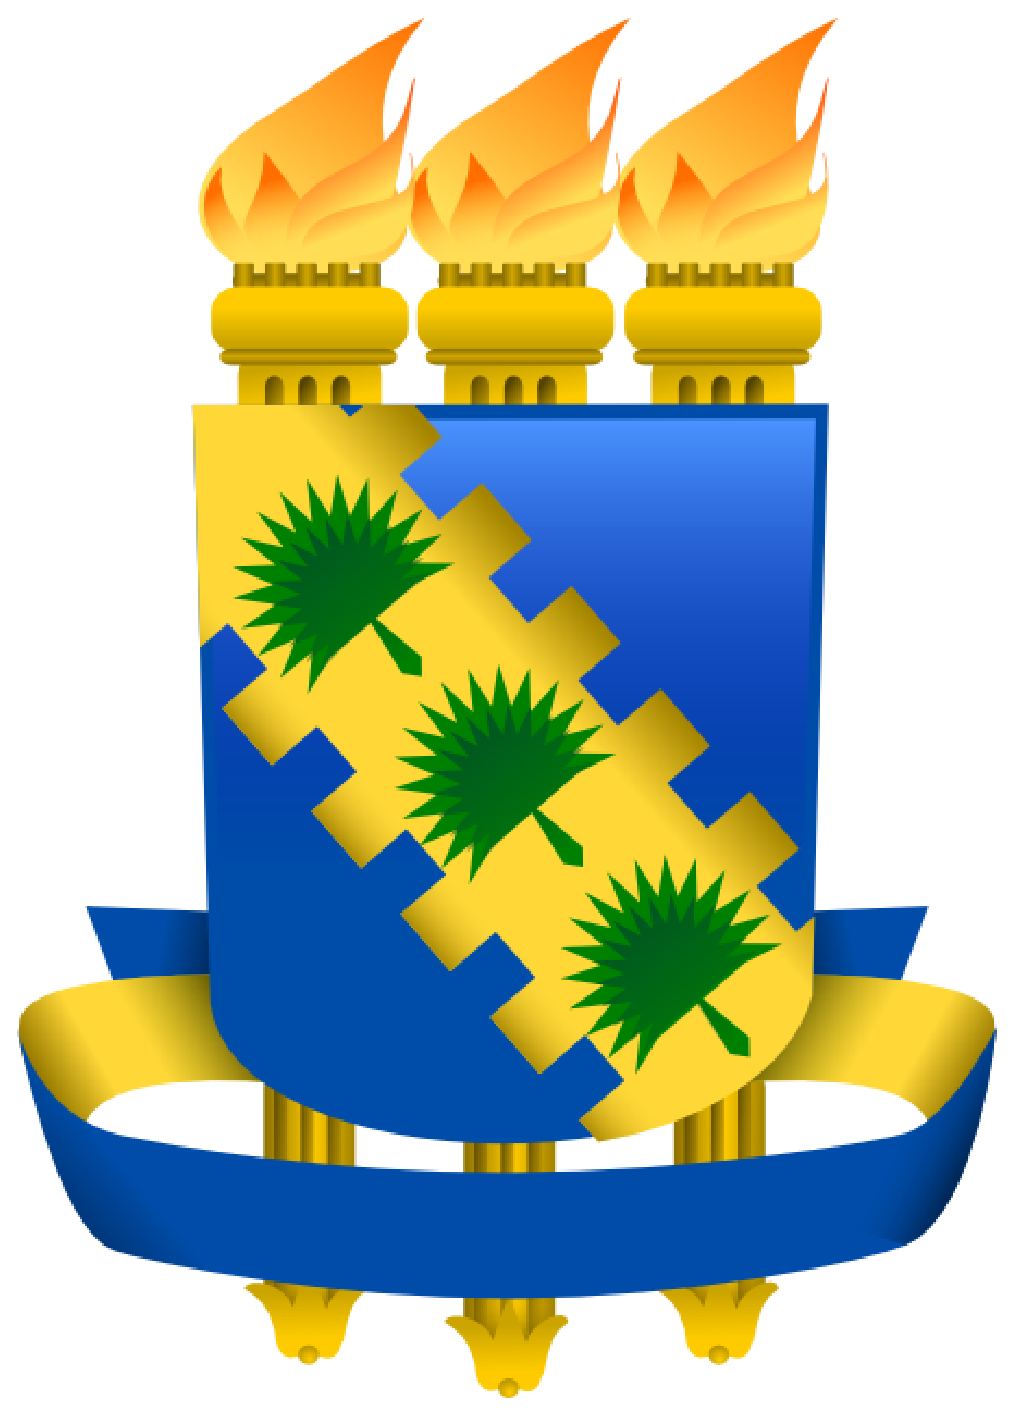
\includegraphics[width=2.5cm]{figs/UFC.eps} \\%
    \textsc{ \autor } \\
     \vspace{.5 cm} \textbf{ \titulo }     \\
\end{center}
    \vspace{.2 cm}
    Esta Monografia foi julgada adequada para a obten��o do diploma de Engenheira do Curso de Gradua��o em Engenharia de Teleinform�tica da Universidade Federal do Cear�.
    \assinatura{\autor}
    \vspace{0.2 cm}
     Banca Examinadora:
     \assinatura{\orientador \\ Orientador}
     \assinatura{\membroa\\}
     \assinatura{\membrob \\}
    \assinatura{\membroc\\}
%     \assinatura{\membrod}
     \vspace{0.2 cm}%\null\vfill%%

\begin{center}
    {\normalsize    Fortaleza, \today}
\end{center}

\frontmatter \pagestyle{roman}
%%%%%%%%%%%%%%%%%%%%%%%%%%%%%%%%%%%%%%%%%%%%%%%%%%%%%%%%%%%%%%%%
%%% RESUMO

% ----------------------------------------------------------------------- %
% Pequeno texto que em poucas palavras consegue expressar o trabalho.
% O resumo deve ser concebido de forma tal que, uma pessoa ao ler o resumo
% possa entender sobre qual assunto este trabalho trata.
%
% Arquivo: resumo.tex
% ----------------------------------------------------------------------- %
\pdfbookmark[1]{Resumo}{CHP:RESUM0}
\chapter*{Resumo}
\label{CHP:RESUM0}
\thispagestyle{empty}
\singlespacing
	\lipsum[3-4]
\onehalfspacing
\pdfbookmark[1]{Abstract}{CHP:ABSTRACT}
\chapter*{Abstract}
\label{CHP:ABSTRACT}%%
\thispagestyle{empty}


\PARstartOne{A} great number of web applications has, for mobile platforms \emph{iOS} and \emph{Android}, some version for mobile systems, which same information is shared on cloud. Some popular social networks like \emph{Twitter} and \emph{Foursquare} has communication interfaces REST as a service to other applications. This paper aims to make a comparative study between iOS and Android applications that use a RESTful web application. To conduct the study, it created a small social network to create quizzes using \emph{Ruby on Rails} and a SaaS service like \emph{Heroku}.


%\PARstartOne{H}{ard} disks are very important elements in any modern computer system and it is advisable to monitor the health of these devices because they are used for applications from personal computers to risk activities. This work aims to build a framework in Linux system using the standard commands \ac{ATA} and \ac{SCSI} to support the development of algorithms for test drives. To demonstrate the use of the framework, algorithms are implemented some test that is compared with diagnostic tools on the market. Finally, these algorithms are embedded in a bootable version of Linux, which allows you to perform during any computers that support booting from a live CD or USB stick, regardless of operating system installed. The test results show the algorithm is very satisfactory, demonstrating the effectiveness of the framework.

%For the development of the work all commands have been developed in ANSI C + + language. Several commands \ac{ATA} and \ac{SCSI} were implemented to support reading, self-testing and other features. Also, the algorithm are implemented from them.
%\newline
%\newline
\noindent \textbf{Keywords: iOS, Android, Mobile, Ruby on Rails, REST, RESTFul}.

%Hard disks are  elements in any modern computer system and it is  to monitor the health of these devices, because they are used for applications from personal computer to risk activities. This work aims to build a framework in Linux system using the standard commands ATA and SCSI to support the development of algoritms for test devices. 
%%%%%%%%%%%%%%%%%%%%%%%%%%%%%%%%%%%%%%%%%%%%%%%%%%%%%%%%%%%%%%%%
%%% DEDICATRIA
% ----------------------------------------------------------------------- %
% Pequena dedicatória ou uma epígrafe (uma citação pertinente ao seu 
% trabalho ou que represente o seu modo de pensar.) 
% 
%
% Arquivo: dedicatoria.tex
% ----------------------------------------------------------------------- %
\thispagestyle{empty}
\vspace*{\fill}

{ \raggedleft


\textit{Dedico este trabalho a ...}

~
}

%%%%%%%%%%%%%%%%%%%%%%%%%%%%%%%%%%%%%%%%%%%%%%%%%%%%%%%%%%%%%%%%
%%% AGRADECIMENTOS
%\chapter{Agradecimentos}
\label{CHP:ACKNOWLEDGMENT}%%
\thispagestyle{empty}
% \PARstartOne{A}{grade\c{c}o}
%Agrade\c{c}o primeiramente ao Pai Celestial por todas as ben\c{c}\~{a}os derramadas sobre mim
%durante toda minha vida.
%
%\`{A} minha esposa que est\'{a} sempre me apoiando desde a escrita da minha Monografia na gradua\c{c}\~{a}o.
%
%Ao Professor Dr. Paulo C\'{e}sar Cortez, meu Orientador Cient\'{\i}fico, pela amizade e a oportunidade de receber um pouco de sua sabedoria, pela disponibilidade
%apresentada e pelas condi\c{c}\~{o}es que me proporcionou para a realiza\c{c}\~{a}o
%deste trabalho.
%
%Ao Rodrigo Costa, pela paci\^{e}ncia e esfor\c{c}o compartilhado auxiliando na orienta\c{c}\~{a}o desse trabalho, e aos demais integrantes do grupo GIHM (Grupo de Inova\c{c}\~{a}o ).
%
%Aos amigos, Auzuir Ripardo, Pedro Pedrosa , Tarique Cavalcante, dentre
%outros integrantes do sub-grupo de pesquisa em Engenharia Biom\'{e}dica do Laborat\'{o}rio de Engenharia de Sistemas de Computa\c{c}\~{a}o, pela amizade e esfor\c{c}o compartilhado durante o curso de mestrado.
%
%Aos engenheiros de desenvolvimento do SIDI (Samsung Instituto de Desenvolvimento para a Inform\'{a}tica), Giovanni, Miguel e Nelson pelo embarque dos algoritmos na plataforma de testes.
%
%Por fim, mas n\~{a}o menos importante, \`{a} Coordena\c{c}\~{a}o de Aperfei\c{c}oamento de Pessoal de N\'{\i}vel Superior (CAPES) e Funda\c{c}\~{a}o Cearense de Apoio ao Desenvolvimento Cient\'{\i}fico e Tecnol\'{o}gico (FUNCAP) pelo suporte financeiro atrav\'{e}s do concedimento da bolsa de Mestrado.


%\textbf{DEDICAT\'{O}RIA}
\thispagestyle{empty}%
\newpage
\null\vfill
\begin{flushright}
%\emph{"Fazer do of\'{\i}cio uma divers\~{a}o levada a s\'{e}rio."}\\Chico Science
\emph{$\ldots$ Cada sonho que voc� deixa pra tr�s, � um peda�o do seu futuro que deixa de existir.}\\
Steve Jobs

%\emph{ "$\ldots$\\All your life, You were only waiting for the moment to arise.\\
%%...
%%All your life, You were only waiting for the moment to be free.
%Black bird fly, black bird fly\\
%Into the light of the dark black night\\$\ldots$" }
%
%\emph{Black Bird - The Beatles}
\end{flushright}
   \vspace{3.0cm}

%% ----------------------------------------------------------------------- %
% Pequena dedicatória ou uma epígrafe (uma citação pertinente ao seu 
% trabalho ou que represente o seu modo de pensar.) 
% 
%
% Arquivo: dedicatoria.tex
% ----------------------------------------------------------------------- %
\thispagestyle{empty}
\vspace*{\fill}

{ \raggedleft


\textit{Dedico este trabalho a ...}

~
}

%%%%%%%%%%%%%%%%%%%%%%%%%%%%%%%%%%%%%%%%%%%%%%%%%%%%%%%%%%%%%%%%
%%% ABREVIA\c{C}\~{O}ES
\begin{singlespace}
    %%%%%%%%%%%%%%%%%%%%%%%%%%%%%%%%%%%%%%%%%%%%%%%%%%%%%%%%%%%%%%%%
    %%% \'{I}NDICE
    %\addtocontents{toc}{\noindent\protect\rule{\textwidth}{.2pt}\par}
    \pdfbookmark[1]{Sum�rio}{sumario_label} %\label{sumario_label}
    \tableofcontents%
    %%%%%%%%%%%%%%%%%%%%%%%%%%%%%%%%%%%%%%%%%%%%%%%%%%%%%%%%%%%%%%%%
    %%% LISTA DE FIGURAS
    \newpage
    %\pdfbookmark[1]{Lista de Figuras}
    \listoffigures%
    \addcontentsline{toc}{chapter}{Lista de Figuras}%
    %%%%%%%%%%%%%%%%%%%%%%%%%%%%%%%%%%%%%%%%%%%%%%%%%%%%%%%%%%%%%%%%
    %%% LISTA DE TABELAS
    \newpage
    \listoftables%
    \addcontentsline{toc}{chapter}{Lista de Tabelas}%
    %%%%%%%%%%%%%%%%%%%%%%%%%%%%%%%%%%%%%%%%%%%%%%%%%%%%%%%%%%%%%%%%
    %%% LISTA DE QUADROS
  %  \newpage
%    \addcontentsline{toc}{chapter}{Lista de Quadros}%
%    \chapter*{Lista de Quadros}%%
%    
Quadro 1

Quadro 2

Quadro 3

    %%%%%%%%%%%%%%%%%%%%%%%%%%%%%%%%%%%%%%%%%%%%%%%%%%%%%%%%%%%%%%%%
    %%% LISTA DE ALGORITMOS
    %    \listofalgorithms%
    %    \addcontentsline{toc}{chapter}{Lista de Algoritmos}%
     %\addtocontents{toc}{\noindent\protect\rule{\textwidth}{.2pt}\par}
    %%%%%%%%
    %%%% NOTA\c{C}\^{A}O
%    \addcontentsline{toc}{chapter}{Lista de S\'{\i}mbolos}%
%    \chapter*{Lista de S\'{\i}mbolos}%%
%    \LTXtable{\textwidth}{pretexto/simbolos}%%
    \newpage
    \addcontentsline{toc}{chapter}{Lista de Siglas}%
    \chapter*{Lista de Siglas}%%
    %\chapter{Fundamenta��o Te�rica} \label{CHP:FUND}

\section{Servi�os PaaS}
\subsection{Defini��o}

Segundo o \ac{NIST}, o termo computa��o em n�vem tem a seguinte defini��o: ``Cloud Computing (pt: computa��o em nuvem) � um modelo que permite, de forma conveniente, o acesso � rede sob demanda para um conjunto compartilhado de recursos de computa��o configur�veis (por exemplo, redes, servidores, armazenamento, aplicativos e servi�os) que podem ser rapidamente provisionados e lan�ados  com o m�nimo de esfor�o de gest�o ou a intera��o de um prestador de servi�os.''. Um dos servi�os definidos � o \ac{PaaS}.

	Ainda de acordo com o \ac{NIST}, o \ac{PaaS} � ``a capacidade fornecida ao consumidor de publicar aplica��es usando linguagem de programa��o, bibliotecas, servi�os suportados pelo provedor''. Com o fornecimento de tal servi�o, o consumidor n�o precisa se preocupar com o controle de certos servi�os de infra-estrutura, como a rede, servidores, sistemas operacionais, armazenamento, ou seja, criam uma camada de abstra��o de servi�os de infra-estrutura.
	
	De acordo com \cite{cloudstack}, servi�os \ac{PaaS} possuem as seguintes caracter�sticas:
\begin{itemize}
\item Servi�os para desenvolver, testar, publicar, hospedar e manter aplica��es de forma integrada;
\item Arquitetura Multi-tenant, onde v�rios usu�rios podem utilizar o mesmo ambiente de desenvolvimento;
\item Constru��o garantindo escalabilidade, incluindo balanceamento de carga (load balancing) e replica��o de dados para recupera��o de falhas (failover);
\item Integra��o com web services e banco de dados atrav�s de padr�es comuns;
\item Suporte para desenvolvimento em equipes, podendo ter ferramentas de planejamento de projetos e de comunica��o;
\item Ferramentas para gerenciamento dos custos.
\end{itemize}

	Ou seja, sistemas \ac{PaaS} s�o �teis para desenvolvedores individuais e startups\footnote{Termo utilizado para designar modelo de n�gocios repet�vel e escal�vel, em um ambiente de extrema incerteza. Normalmente, projetos ou empresas startups est�o associadas as �reas de tecnologia.}, pois fornecem facilidade de publica��o sem os custos e complexidades de hardwares e softwares inerentes a uma aplica��o web comum \cite{guardianstartup}.
	
\subsection{Heroku}

	O \emph{Heroku} � uma plataforma cloud de servi�os \ac{PaaS} montado sobre o \emph{Amazon EC2}, existente desde junho de 2007. Possui suporte para as seguintes linguagens: Ruby, Java, Node.JS, Scala, Clojure, Python e PHP. Internamente, funciona sobre o sistema operacional Ubuntu.

	Inicialmente, o \emph{Heroku} foi desenvolvido com suporte exclusivo para a linguagem Ruby. Em julho de 2011, Matz Matsumoto, criador do Ruby, entrou para a empresa como Arquiteto-chefe e, nesse mesmo m�s, passou a dar suporte tamb�m para Node.js e Clojure.
Em setembro de 2011, a rede social \emph{Facebook} fez uma parceria com o \emph{Heroku} a fim de facilitar a publica��o de aplicativos para sua pr�pria plataforma \cite{faceheroku}. Em poucos passos, � poss�vel criar uma aplica��o no Facebook e no Heroku, simultaneamente.
O \emph{Heroku} usa uma unidade de m�quina virtual chamada ``Dyno'' com 4 cores e at� 512mb de RAM.

	

\section{REST}
 O \ac{REST} foi definido em uma tese de doutorado por Roy Fielding da seguinte maneira: 
``O REST  � pretendido como uma imagem do design da aplica��o se comportar�: uma rede de websites (um estado virtual), onde o usu�rio progride com uma aplica��o selecionando as liga��es (transi��es do estado), tendo como resultado a p�gina seguinte (que representa o estado seguinte da aplica��o) que est� sendo transferida ao usu�rio e apresentada para seu uso.''

	De modo geral, o \ac{REST} � uma interface de comunica��o onde h� um provedor de servi�os e um consumidor. Tal interface pode ser descrita utilizando \ac{XML}, \ac{HTTP}, \ac{YAML}, \ac{JSON} ou at� mesmo texto puro, de modo a n�o utilizar trocas de mensagens complexas como o \ac{SOAP}. 

O \ac{REST} possui alguns princ�pios, a saber:
\begin{itemize}
\item Modelo provedor/consumidor Stateless (sem estado): cada mensagem \ac{HTTP} trocada possui todas as informa��es necess�rias para a comunica��o, ou seja, nenhuma das partes necessita gravar estado da comunica��o. Em sistemas web, � comum o uso de cookies para manter o estado da sess�o; j� em sistemas mobile, � comum utilizarmos um token de autentica��o, com a mesma finalidade.

\item Opera��es \ac{HTTP}: de modo a diminuir o tr�fego de dados, s�o utilizados m�todos \ac{HTTP} para acessar os recursos de informa��o. As opera��es mais utilizadas s�o o GET, PUT, POST e DELETE. Em sistemas \ac{REST}, � comum combinar tais m�todos com opera��es de CRUD (create, read, update e delete), que faz persist�ncia de dados em um determinado recurso ou entidade.

\item Identifica��o de recursos: As URLs identificam cada uma das entidades e seus elementos, ficando a cargo da opera��o \ac{HTTP} definir a a��o a ser feita com cada um dos recursos ou elementos.

\item Uso de hiperm�dia: As trocas de mensagem de comunica��o � feita utilizando, no corpo da mensagem \ac{HTTP}, uma linguagem de marca��o, conforme j� citado anteriormente. Por�m, n�o h� uma restri��o geral quanto ao uso, podendo ser usada linguagens pr�prias (texto puro).

\end{itemize}
\subsection{RESTful}

	Em uma arquitetura julgada como \emph{RESTful}, o m�todo desejado � informado dentro do m�todo \ac{HTTP}, contido no header do mesmo. Al�m disso, o escopo da informa��o � colocado na \ac{URL}, o que torna uma ``combina��o poderosa''. Por defini��o, uma aplica��o deixa de ser RESTFul caso o m�todo \ac{HTTP} n�o combine com o m�todo da informa��o, ou seja, com a funcionalidade esperada para aquela estrutura de dados. \cite{restfulws}

\section{JSON}
\subsection{Introdu��o}
\ac{JSON} � um padr�o aberto de texto para representar estruturas de dados, de forma intelig�vel para humanos.  Sua origem � a linguagem javascript, e seu formato est� descrtio no RFC 4627.

\subsection{Defini��o}
	O \ac{JSON} � um dos formatos mais usados na serializa��o e transmiss�o de dados estruturados pela internet,ao lado do \ac{XML} e \ac{YAML}, sendo muito usado em sistemas orientados a servi�o / webservice. Muitas linguagens e frameworks, como o Foundation (iOS) e o Android, d�o suporte para esse padr�o, atrav�s de parsers para constru��o e consumo.
De acordo com \cite{restfulws}, ``� muito mais f�cil para um browser lidar com uma estrutura javascript oriunda de uma estrutura JSON do que a partir de um documento XML''. Ainda de acordo com a fonte, cada web browser oferece uma interface JavaScript diferente para seus parsers XML, enquanto um objeto \ac{JSON}, que por defini��o � um objeto JavaScript, ser� interpretado da mesma maneira em qualquer interpretador JavaScript. O \ac{JSON} � uma alternativa mais leve para serializa��o de dados do que o \ac{XML}, definido pelo \ac{XML} Schema. 

\subsection{compara��o com XML}
	\ac{JSON} e \ac{XML} s�o dois formatos de manipula��o de informa��es que podem ser usados com o mesmo objetivo, mas possuem implementa��es e aplica��es distintas. 

	No artigo \cite{comparexmljson}, � feito um estudo considerando a hip�tese de que n�o h� diferen�a em rela��o ao tempo de transmiss�o e os recursos utilizados entre \ac{JSON} e XML.A fim de realizar o estudo, foi criado um ambiente operacional consistindo de uma aplica��o cliente/servidor em Java, onde o servidor escuta uma porta e o cliente conecta a ela. 

	No referido teste, foram utilizadas as seguintes m�tricas: n�mero de objetos enviados, tempo total para enviar o n�mero de objetos, tempo m�dio de transmiss�o, uso da CPU pelo usu�rio, uso da CPU pelo sistema e o uso de mem�ria.

	De acordo com a conclus�o do artigo, codifica��o \ac{JSON} �, em geral, mais r�pida e consome menos recursos que a codifica��o XML, o que nega a hip�tese de igualdade de escolha entre as duas tecnologias. Ou seja, em um ambiente onde � necess�ria velocidade e os recursos s�o limitados, como sistemas m�veis, � prefer�vel utilizar \ac{JSON}.

\subsection{Estrutura}
	De acordo com W3resource \cite{w3json}, o \ac{JSON} suporta duas grandes estruturas de informa��o: cole��o de pares chave/valor e listas ordenadas de valores. Ambas estruturas s�o tamb�m suportadas pela maioria das linguagens de programa��o modernas, o que refor�a a ideia de ser uma boa escolha de linguagem para transmiss�o de informa��es.
	
	O \ac{JSON}possui alguns tipos de dados, a saber:
\begin{itemize}
\item Objetos: um objeto come�a e termina com '{' e '}', contendo um n�mero de pares chave/valor.  A separa��o entre uma chave e um valor � feita com o caractere ':',  e a separa��o entre pares � feita com ','. O valor de um par pode ser qualquer estrutura JSON.
\item Arrays: Um array come�a e termina com '[' e ']'. Entre eles, s�o adicionados certo numero de valores, separados por ','. 
\item Valores: os valores podem ser string, numero, objeto, array, valor booleano ou null.
\end{itemize}
Exemplo de c�digo JSON:

\begin{lstlisting}
{
    "firstName": "Bidhan",
"lastName": "Chatterjee",
    "age": 40,
    "address": {
        "streetAddress": "144 J B Hazra Road",
        "city": "Burdwan",
        "state": "Paschimbanga",
        "postalCode": "713102"
    },
    "phoneNumber": [
        {
            "type": "personal",
            "number": "09832209761"
        },
        {
            "type": "fax",
            "number": "91-342-2567692"
        }
    ]
}
\end{lstlisting}

\section{Ruby on Rails}

\subsection{Ruby}
	Ruby � uma linguagem orientada a objetos, com tipagem forte e din�mica, criada por Yukihiro Matsumoto (Matz) em 1995. 
	
	Segundo \cite{caelum}, uma de suas principais caracter�sticas � sua expressividade, ou seja, a facilidade de ser lida e entendida, o que facilitaria o desenvolvimento de sistemas escritos por ela.
	
	O livro \cite{rails3} lista algumas das caracter�sticas mais importantes do Ruby, a saber:
\begin{itemize}
\item � uma linguagem interpretada, ou seja, um interpretador l� o c�digo e decide como executar em tempo de execu��o. Por consequ�ncia, um sistema em Ruby pode se tornar um pouco mais lento, por�m, � not�vel o ganho em flexibilidade.
\item Possui uma sintaxe de linguagem flex�vel, fazendo com que a curva de aprendizado seja menor em rela��o a outras linguagens. Um exemplo cl�ssico � a n�o-necessidade (opcional) de escrever par�nteses ao redor dos par�metros de um m�todo. Entretanto, podem surgir erros misteriosos por n�o colocar par�nteses em algumas situa��es amb�guas.
\item Possui uma tipagem din�mica, ou seja, n�o � necess�rio especificar o tipo de informa��o que ser� guardado em cada vari�vel. Isso torna a abordagem bem mais flex�vel, tornando as opera��es dependentes do pr�prio contexto. Entretanto, problemas podem ocorrer justamente por isso: comportamentos inesperados.
\item Suporte a blocos e closures,
\end{itemize}
	
	Atualmente, Ruby encontra-se entre as linguagens de programa��o mais populares, ocupando a posi��o 11� no �ndice Tiobe\footnote{O �ndice TIOBE mede, mensalmente, a popularidade de uma determinada linguagem de programa��o, baseado no numero de engenheiros qualificados, cursos, vendedores e buscas nos principais motores de busca. Pode ser encontrado em \url{http://www.tiobe.com/index.php/content/paperinfo/tpci/index.html} }.  Grande parte desse sucesso deve-se ao framework Rails, implementado como solu��o web utilizando Ruby.

\subsection{Rails}
	O Ruby on Rails, tamb�m chamado Rails ou RoR, � um framework de desenvolvimento web de c�digo aberto que tem como premissa aumentar a velocidade e a facilidade no desenvolvimento de aplica��es web orientados a banco de dados.  Foi lan�ado oficialmente em Julho de 2004 pelo seu criador David H. Hansson, estando atualmente na vers�o 3.2.11, com a 4� vers�o em desenvolvimento \cite{rails4}.  
	
	O Rails � um framework full-stack, ou em portugu�s, pilha completa. Isso significa que, com ele, � poss�vel desenvolver a aplica��o por completo, desde o desenvolvimento dos layouts das paginas, a manuten��o do banco de dados. Al�m disso, o Rails enfatiza o uso de alguns padr�es de engenharia de software, a saber:
	
\begin{itemize}
\item Active record: padr�o de projeto para armazenamento de dados em banco de dados relacionais.  A interface de um certo objeto deve incluir fun��es de CRUD,  como inserir, atualizar, apagar e algumas fun��es de consulta. Cada tabela de um banco de dados � embrulhada (wrapped) em um uma classe, sendo cada instancia dessa classe um registro (tupla) �nico na tabela.  Esse conceito est� definido em \cite{fowler}.
\item Conven��o sobre configura��o: modelo de desenvolvimento de software que busca diminuir o n�mero de decis�es que os desenvolvedores precisam tomar, ou seja, o desenvolvedor n�o precisa definir aspectos convencionais da aplica��o. Em Rails, � f�cil perceber esse padr�o na escolha dos nomes das tabelas: se um modelo chama-se ``Usuario'', a tabela correspondente se chamar� ``Usuarios'' e, se existir uma rela��o entre usu�rios e contas (m:m), a nova tabela ser� denominada, automaticamente, $usuarios_contas$.
\item \ac{DRY}: O objetivo principal � reduzir a repeti��o de informa��o de qualquer tipo. Esse conceito incentiva o bom uso da reutiliza��o de c�digo, que � tamb�m uma das principais vantagens da orienta��o a objetos.
\item \ac{MVC}: esse padr�o de arquitetura de software separa a aplica��o em tr�s camadas: uma contendo a l�gica da aplica��o e regra de neg�cios, chamada model; uma contendo a entrada e sa�da de dados com o usu�rio, chamada view; uma interligando ambas, de maneira a manipular dados da view para o model entender e vice-versa, chamada controller. O principal objetivo dessa arquitetura � a reusabilidade de c�digo e a separa��o de conceitos \cite{mvc}.
\end{itemize}


 	De acordo com \cite{caelum}, a estrutura a qual o Rails � feito permite que as funcionalidades de um sistema possam ser implementadas de maneira incremental, por conta dos padr�es e conceitos supracitados. Por conseq��ncia, isso tornaria o Rails uma boa escolha para projetos e empresas que adotam metodologias �geis no desenvolvimento da aplica��o.

 	O Ruby � uma linguagem interpretada. Antes de se tornar popular, existia apenas um interpretador dispon�vel, escrito em C pelo pr�prio criador da linguagem. Hoje em dia, o interpretador mais conhecido � o 1.9 ou YARV (Yet Another Ruby VM), para a vers�o mais atualizada e est�vel (Ruby 1.9.3.).
 	
	Existem outros interpretadores Ruby famosos, como:
 \begin{itemize}
 \item JRuby: implementa��o alternativa que permite usar a \ac{JVM} do Java para interpetar c�digo Ruby. Uma de suas principais vantagens � a interoperabilidade com c�digo Java existente, al�m de aproveitar as vantagens j� maduras do java: garbage collector, threas nativas, etc.
 \item IronRuby: Implementa��o .Net da linguagem, mantido pela pr�pria Microsoft
 \item Rubinius: Traz id�ias de m�quinas virtuais do SmallTalk e � implementada em C/C++.
 \end{itemize}
 \section{Smartphones}

 	O mercado de smartphones est� crescendo cada vez mais. Estima-se que no �nicio de 2012 o n�mero de celulares inteligentes tenha atingido a marca de 1 bilh�o de unidades vendidas e, segundo proje��es, esse n�mero deve dobrar em 2015 \cite{yahoosmart}. 
 	
	Embora o n�mero de smartphones seja expressivo, ele ainda � pequeno se comparado ao n�mero de pessoas que possuem um aparelho celular: 3 bilh�es. Isso significa que ainda h� muito espa�o para crescimento, em particular em mercados emergentes como a China, �ndia e �frica.
 	
	Usualmente, um smartphone possui alguns recursos de ponta, como c�mera, bom reprodutor de m�dia, bom processamento gr�fico para jogos, bluetooth, GPS, acesso a internet via wi-fi e 3G/4G, \ac{NFC}, um bom sistema operacional, entre outros. 
 Atualmente, os sistemas operacionais mais populares para smartphones s�o: Android, iOS (Apple), Blackberry OS (RIM), Bada (Samsung), Symbian e Windows Phone 7 (Microsoft). A distribui��o do mercado, no Q3 de 2012, pode ser vista no seguinte gr�fico:
 \begin{figure}[H]
   % Requires \usepackage{graphicx}
   \centering
   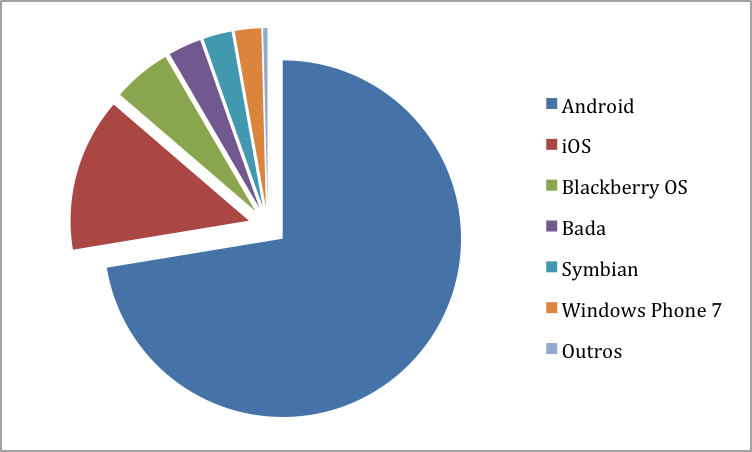
\includegraphics{figs/smartpizza.png}\\
   \caption{ MarketShare Q3 2012}
   \label{FIG:smartpizza}
 \end{figure}
 Fonte: \cite{neowin}
 
 Notadamente, o Android e o iOS s�o as plataformas mais populares. O grande diferencial entre o marketshare desses dois sistemas s�o o segmento de mercado: enquanto o Android atua em todos os segmentos, desde celulares \emph{low-end} aos celulares de ponta, o iOS atua somente com celulares de ponta, chamados \emph{high-end}. Outro fato a considerar � que, nesse gr�fico, n�o s�o considerados outros dispositivos, como tocadores de m�sica e \emph{tablets}.

 \section{iOS}
 \subsection{Vis�o Geral}

 O iOS � um sistema operacional para dispositivos m�veis, lan�ado pela Apple em 2007. Inicialmente, foi desenvolvido para o iPhone, sendo posteriormente aproveitado nos dispositivos iPod Touch, iPad e Apple TV. Ele � um sistema operacional licenciado para rodar apenas em hardware produzido pela Apple, otimizado para a arquitetura de processadores ARM.
 
 Sua entrada de dados � feita de forma direta, atrav�s de multi- toques. Esses toques podem ser desde encostar o dedo, similar a um clique do mouse, at� balan�ar o aparelho, de modo a utilizar seu aceler�metro. Todos os controles de entrada de dados s�o controlados pela \ac{GUI} Cocoa Touch.
 
 O livro \cite{usecabecaiphone} cita que o iPhone revolucionou a maneira de ver um celular: ele �, atualmente, uma plataforma de jogos, um organizador pessoal, um navegador (browser) completo e, claro, um celular. Muito de seu sucesso deve-se ao sucesso da loja virtual ``App Store'', de m�dias e aplicativos, que abriu oportunidade para desenvolvedores independentes competirem em escala mundial com grandes empresas de software. 

 \subsection{Linguagem: Objective-c}
 A programa��o nativa em iOS utiliza uma linguagem de programa��o chamada Objective-C, com o \emph{framework} Foundation. 
 
 O Objective-C � uma linguagem de programa��o reflexiva e orientada a objeto, com origens no SmallTalk e no C. Foi criada no in�cio da d�cada de 80 por Brad Cox e Tom Love, mas somente se tornou popular quando foi licenciada pela NeXT, de Steve Jobs, em 1988. Atualmente � a principal linguagem utilizada para desenvolvimento para Mac OS X.
 
 Como o Objective-C foi construido sobre C, qualquer c�digo C pode ser compilado com um compilador Objective-C. Por defini��o, � uma camada sobre o C que aceita orienta��o a objetos, atrav�s de mensagens.
 
 Em linguagens com ``message parsing'', m�todos n�o s�o chamados de objetos, mas sim mensagens s�o enviadas ao objeto. Essa diferen�a implica em como o c�digo referenciado pelo m�todo ou nome da mensagem � executado. Em nosso caso, o ``alvo'' da mensagem � resolvido em tempo de execu��o, com o objeto receptor interpretando a mensagem.

 \subsection{Ciclo de vida}
 O ciclo de vida constitui uma sequ�ncia de eventos entre o in�cio e a finaliza��o da aplica��o. Um aplicativo iOS come�a quando o usu�rio toca o �cone da mesma na home do dispositivo. Feito isso, o sistema operacional inicia alguns procedimentos de renderiza��o e chama a fun��o principal (main.m) do aplicativo.
 
 Uma vez iniciado, o comando da execu��o passa a ser do UIKit, framework de controle do iOS, que carrega a interface gr�fica e l� o loop de eventos. Durante o loop, o UIKit delega cada evento a seu respectivo objeto e responde aos comandos emitidos pelo aplicativo. Quando o usu�rio realiza uma a��o que causa um evento de sa�da, o UIKit notifica a aplica��o e inicia o processo de sa�da.


 \section{Android}

 \subsection{Vis�o Geral}
 	O Android � a resposta do Google para ocupar o segmento de mercado de sistemas operacionais para plataformas m�veis. Consiste em um novo sistema baseado no sistema operacional Linux, com diversas aplica��es j� instaladas, al�m de um ambiente de desenvolvimento forte e flex�vel. 
	
 	De acordo com \cite{lecheta}, o Android causou um grande impacto quando foi anunciado, em especial pelas empresas que estavam por tr�s de seu desenvolvimento: Google, Motorola, LG, Samsung, Sony, entre muitas outras. A esse grupo de empresas, denominado \ac{OHA}, coube � padroniza��o de uma plataforma de c�digo aberto e livre para celulares, com o objetivo de atender a demanda do mercado atual.
	
 	Um dos pontos fortes do Android � seu sistema flex�vel: � f�cil integrar aplica��es nativas com a sua aplica��o, ou at� mesmo substituir algumas dessas aplica��es nativas pela sua pr�pria. Isso gera um grande apelo para empresas de telefonia, que podem usar dessa personaliza��o para lan�arem suas pr�prias vers�es de aparelhos Android personalizados.
	
 	O grande foco do sistema � a intera��o entre aplicativos: agenda, maps, contatos s�o facilmente alcan��veis por qualquer aplica��o. Essa funcionalidade � realizada por um recurso chamado Intent.%, que ser� abordado em cap�tulos posteriores.
	
 	Outro ponto forte do Android � que seu sistema operacional � baseado no Linux (baseado no kernel 2.6), ou seja, ele mesmo se encarrega de gerenciar a memoria em uso e os processos. Isso faz com que seja poss�vel rodar mais de uma aplica��o (genuinamente) ao mesmo tempo, fazendo com que outros aplicativos rodem em segundo plano durante outros servi�os, como ao atender um telefonema ou acessar a internet.  
	
 	O que � dito como vantagem tamb�m � apontado, fatalmente, como um problema: uma vez que aplicativos podem rodar em segundo plano, aplicativos maliciosos tamb�m podem ser rodados em segundo plano. Durante muito tempo, aplicativos desse tipo podiam ser encontrados para download no Android Market (atualmente Google Play), havendo hoje uma melhor sele��o dos aplicativos que de fato est�o sendo disponibilizados na loja.

 \subsection{Linguagem: Java} 
 	A linguagem nativa de programa��o para Android � o Java, utilizando o framework Android criado pela Open Handset Alliance (OHA).
 	O Java � uma linguagem de prop�sito geral, concorrente e orientada a objetos. Sua primeira vers�o foi lan�ada em 1995 pela Sun Microsystems e, atualmente, encontra-se em sua s�tima vers�o, sendo mantida pela Oracle. 
	
 	Atualmente, � uma das linguagens de programa��o mais populares do mundo, ocupando o 2� lugar no �ndice TIOBE. Devido a isso, h� um grande n�mero de desenvolvedores que possuem o pr�-requisito b�sico para iniciar programa��o para Android: o dom�nio da linguagem.
	
 	O grande sucesso do Java � normalmente creditado a sua capacidade de funcionar nos mais diversos ambientes, desde micro-sistemas como cart�es de cr�dito a grandes plataformas web. Isso � devido a implementa��o de sua m�quina virtual, que � capaz de rodar nas mais diversas plataformas. 


 \subsection{Ciclo de vida}
 	 O ciclo de vida de uma aplica��o Android � controlado por uma Activity, a qual tamb�m gerencia a interface com o usu�rio, recebe requisi��es, realiza o tratamento e processa.
	 
 	Toda Activity possui os seguintes m�todos de controle, a saber:
 \begin{itemize}
 \item onCreate(): � o primeiro m�todo a ser executado em uma Activity. Usualmente � o m�todo respons�vel por carregar os layouts XML e inicializar atributos de classe e outros servi�os.
 \item onStart(): � chamado imediatamente chamado ap�s o onCreate(). Diferentemente deste, � chamado toda vez que a Activity volta a ter foco ap�s um per�odo em background.
 \item onResume(): Assim como o onStart(), � chamado no in�cio da Activity e, tamb�m, quando a mesma volta a ter foco. A diferen�a entre ambos � que o onStart() s� � invocado quando a Activity n�o est� mais vis�vel, enquanto o onResume() � chamado toda vez que retorna o foco.
 \item onPause(): � a primeira fun��o a ser chamada quando a Activity perde o foco.
 \item onStop(): � chamado quando uma Activity � substitu�da por outra Activity
 \item onDestroy(): � o �ltimo m�todo a ser executado. Quando o onDestroy() � executado, a Activity � considerada ``morta'' e fica pronta para ser removida pelo Garbage Collector.
 \item	onRestart(): Chamado quando a Activity sai do estado de ``stop''; ap�s sua execu��o, � chamado o m�todo onStart().
 \end{itemize}

 \section{Redes Sociais}  ser� que vale mesmo a pena falar sobre isso?
 \section{Resumo do Cap�tulo}

 	Neste cap�tulo foram abordadas as tr�s principais tecnologias necess�rias para o desenvolvimento deste projeto: computa��o em nuvem, web services e computa��o m�vel. Tais tecnologias foram aprofundadas em um n�vel o qual fornecessem ao leitor os pr�-requisitos para a compreens�o do restante do projeto, o qual ser� apresentado nos cap�tulos posteriores.
 
%\pdfbookmark[1]
\begin{acronym}

% Meus
\acro {CSS}{\emph{Cascading Style Sheets}}
\acro {DRY}{\emph{don't repeat yourself}}
\acro {GUI}{\emph{Graphic User Interface}}
\acro {HTML}{\emph{HyperText Markup Language}}
\acro {HTTP}{\emph{Hypertext Transfer Protocol}}
\acro {JSON}{\emph{JavaScript Object Notation}}
\acro {JVM}{\emph{Java Virtual Machine}}
\acro {IDE}{\emph{Integrated Development Environment}}
\acro {MVC}{\emph{Model View Controller}}
\acro {NFC}{\emph{Near Field Communication}}
\acro {NIST}{\emph{National Institute of Standarts and Technology}}
\acro {OHA}{\emph{Open Handset Alliance}}
\acro {PaaS}{\emph{Platform as a Service}}
\acro {REST}{\emph{Representational State Transfer}}
\acro {SGBD}{\emph{Sistema de Gerenciamento de Banco de Dados}}
\acro {SOAP}{\emph{Simple Object Access Protocol}}
\acro {SSH}{\emph{Secure Shell}}
\acro {TDD}{\emph{Test Driven Development}}
\acro {URL}{\emph{Uniform Resource Locator}}
\acro {XML}{\emph{Extensible Markup Language}}
\acro {YAML}{\emph{YAML Ain't Markup Language}}
\acro {YARV}{\emph{Yet Another Ruby VM}}

\end{acronym} 
    %\LTXtable{\textwidth}{pretexto/siglas}%%
    %GATHER{pretexto/simbolos.tex}%%
    %GATHER{pretexto/siglas.tex}%%
\end{singlespace}

\pagestyle{capitulo} \setlength{\parskip}{1ex plus 0.5ex}
%%%%%%%%%%%%%%%%%%%%%%%%%%%%%%%%%%%%%%%%%%%%%%%%%%%%%%%%%%%%%%%%
%%% CAP�TULO 1: INTRODU��O
\mainmatter
\chapter{Introdu��o} \label{CHP:INTRO}

\section{Motiva��o}

\section{Objetivos}

Os objetivos gerais e espec�ficos desta monografia, s�o apresentados a seguir.

\subsection{Objetivos Gerais}

\subsection{Objetivos Espec�ficos}



\section{Organiza��o do Texto}





%%%%%%%%%%%%%%%%%%%%%%%%%%%%%%%%%%%%%%%%%%%%%%%%%%%%%%%%%%%%%%%
%%%% CAP�TULO 2: Discos R�gidos
\chapter{Discos R�gidos} \label{CHP:HD}%%

Neste cap�tulo, a evolu��o dos discos r�gidos � descrita de maneira breve para contextualizar o leitor quanto �s tecnologias utilizadas atualmente e ao seu funcionamento.

\section{Introdu��o}
%Vivemos em uma era da tecnologia da informa��o onde cada aspecto de nossa vida passa por algum tipo de processamento ou armazenamento de informa��es.

Os sistemas modernos de computa��o usam diferentes tecnologias para armazenar estas informa��es, seja temporariamente ou permanentemente. Essas tecnologias podem ser mem�rias de estado s�lido, como \ac{ROM}, \ac{RAM} e mem�rias \emph{Flash},  armazenamento magn�tico, como \ac{HDD}, \emph{floppy disk} e \emph{tape}, ou armazenamento �ptico, como \ac{CD-ROM}, \ac{DVD}, \ac{BD} e \ac{HD-DVD}.

Os discos r�gidos desempenham um grande papel neste desenvolvimento tecnol�gico.  Atualmente, eles tanto podem ser dispositivos de armazenamento magn�tico como os \acp{HDD}, quanto circuitos de mem�ria \emph{Flash}, no caso dos \acp{SSD} atuais, ou ainda dispositivos h�bridos \cite{HD:hibrido}. Os principais fatores considerados na escolha entre essas tecnologias s�o o custo, a taxa de transfer�ncia de dados, o tempo de acesso e a confiabilidade \cite{Mamun:2007}.

A pir�mide de hierarquia de armazenamento, Figura \ref{FIG:PIRAMIDE2}, descreve uma hierarquia de tecnologias de mem�ria em fun��o do custo, da capacidade de armazenamento e do tempo de acesso. Nela, os dois principais tipos de discos r�gidos, \ac{HDD} e \ac{SSD}, se encontram na camada intermedi�ria.

 A regi�o superior da pir�mide cont�m registradores do processador, mem�ria cache e mem�ria \ac{RAM}, que se caracterizam pelo alto custo, rapidez no acesso aos dados e baixa capacidade de armazenamento. J� a regi�o intermedi�ria cont�m mem�rias Flash, das quais s�o feitos os \acp{SSD}, discos magn�ticos e discos �pticos, que possuem um custo menor em compara��o �s mem�rias internas, maior capacidade de armazenamento e menor velocidade no acesso aos dados. Na regi�o inferior se encontram fitas magn�ticas, dispositivos de acesso sequencial usados para c�pias de seguran�a.

\begin{figure}[htb]
  \centering
  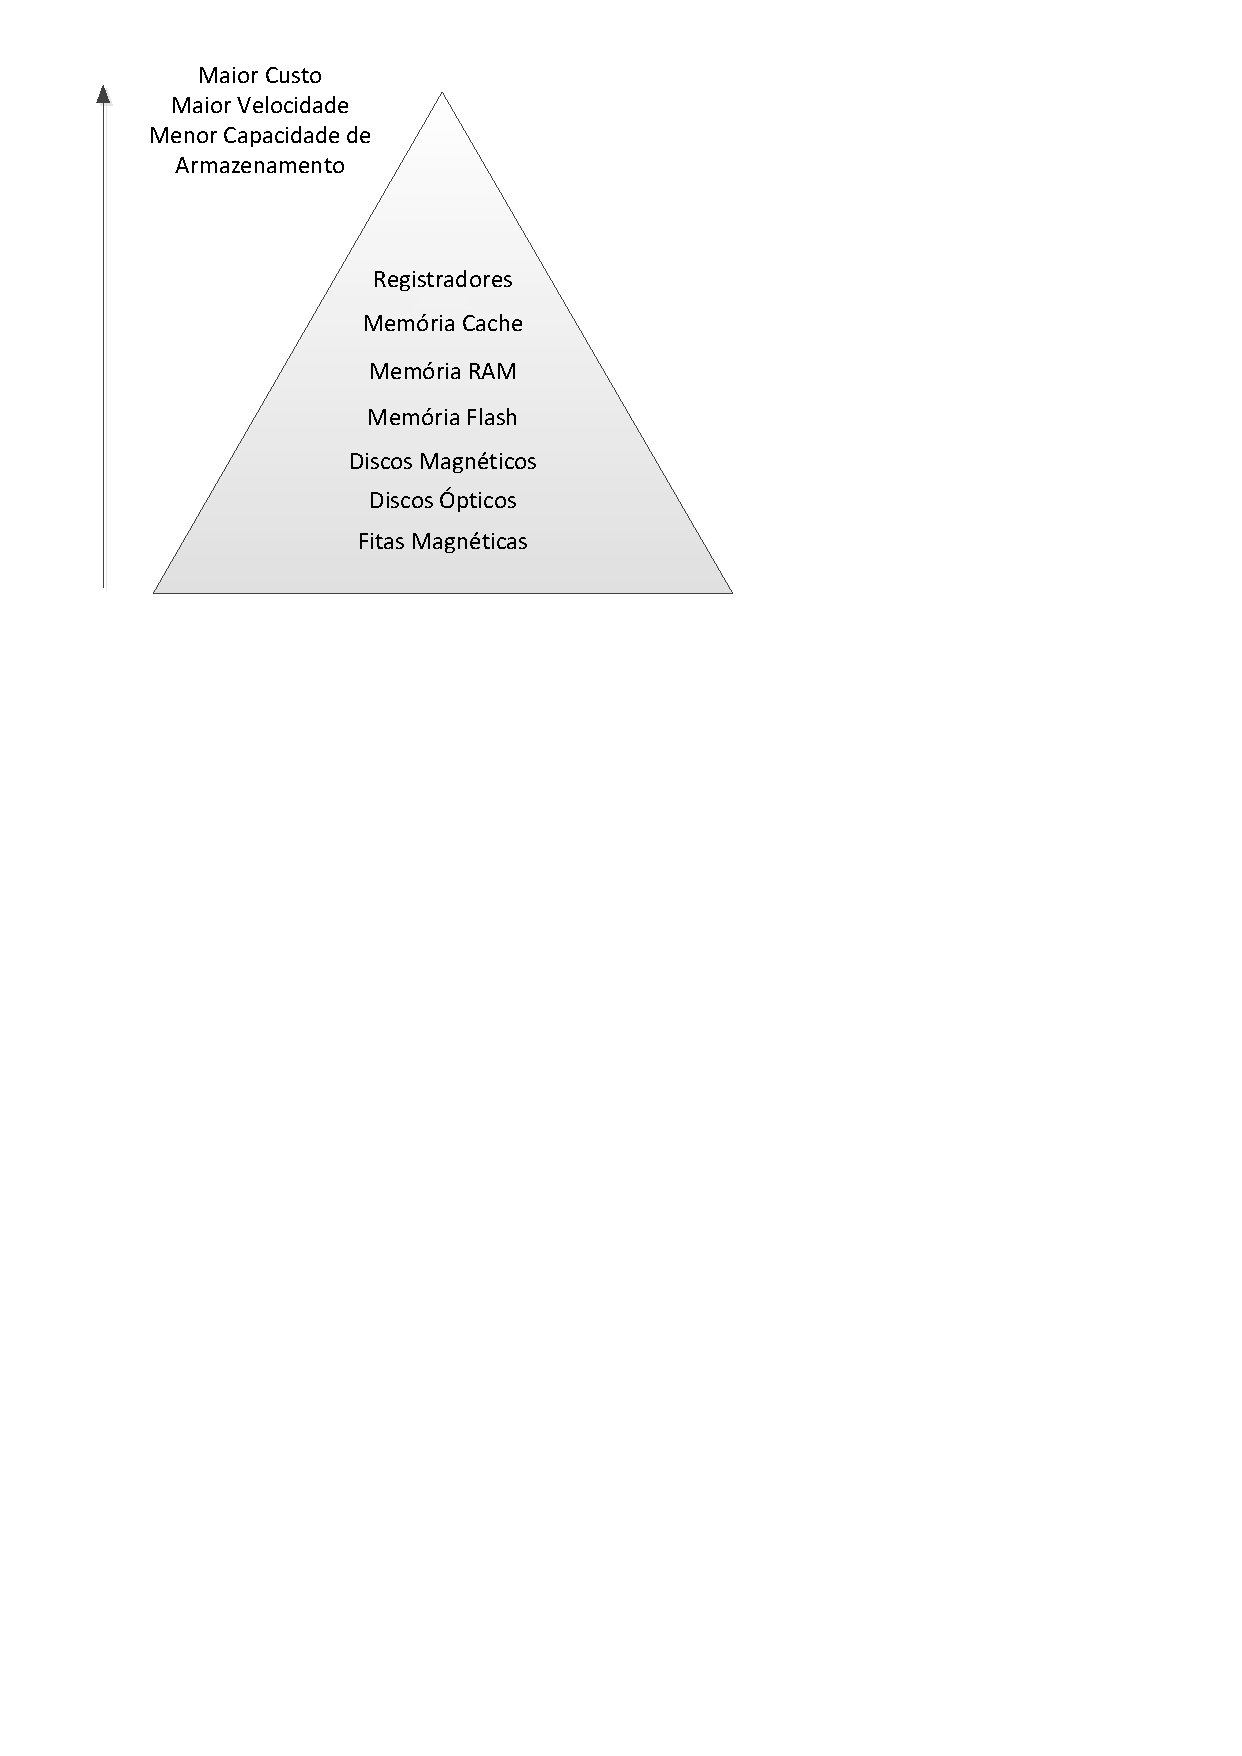
\includegraphics[scale=0.8]{figs/piramide.pdf}
  \caption{Pir�mide Hier�rquica de Armazenamento, adaptada de \cite{Mamun:2007}}
  \label{FIG:PIRAMIDE2}
\end{figure}


\section{Hist�rico}
 O disco r�gido, tamb�m conhecido como \ac{DASD}, em refer�ncia � capacidade de acesso direto, foi um dos dispositivos que mais evoluiu na hist�ria da computa��o.

Em pouco mais de 5 d�cadas, a ind�stria de armazenamento de dados evoluiu de um grande aparato de 50 discos de 24 $in$ de di�metro (aproximadamente 61 cm), com uma capacidade total de 5 MB para discos que armazenam at� 4 TB em discos de 3,5 $in$ de di�metro (pouco menos de 9 cm). Esta enorme evolu��o se tornou poss�vel gra�as a avan�os em diversas �reas do conhecimento incluindo: materiais, tribologia\footnote{Tribologia � a ci�ncia que estuda a intera��o de superf�cies, submetidas a cargas e a movimentos relativos.}, mec�nica, mecatr�nica, processamento de sinais  e eletr�nica, \cite{Harker:1981}.

Os primeiros \acp{HD} eram significativamente diferentes dos que usamos agora, n�o apenas em rela��o ao tamanho, mas em aspectos como capacidade de armazenamento, taxa de transfer�ncia de dados e tecnologia utilizada.

Os \acp{HDD} e \acp{SSD} s�o contempor�neos e foram desenvolvidos pela \ac{IBM}\footnote{A IBM foi o novo nome dado � C-T-R(Computing-Tabulating-Recording Company), empresa fruto da fus�o de outras tr�s empresas entre elas a \emph{Tabulating Machine Company}, fundada por Herman Hollerith, especializada no processamento de dados de cart�es perfurados.}, empresa que come�ou a se destacar no in�cio do s�culo XX atrav�s do desenvolvimento de m�quinas mec�nicas e el�tricas, como calculadoras de repeti��o e m�quinas datilografia, e que foi respons�vel por muitos avan�os na computa��o.

As primeiras m�quinas utilizavam cart�es e fitas de papel para codificar e para armazenar informa��es, mas, entre outras desvantagens, n�o havia mem�ria \ac{RAM} suficiente e o \emph{software} e dados iniciais precisavam ser carregados cada vez que a m�quina era ligada.

Havia a necessidade de mem�rias mais eficientes, tempor�rias e permanentes. Ent�o a \ac{IBM} come�ou a desenvolver mem�rias alternativas, principalmente baseadas em magnetismo. Ela desenvolveu os discos magn�ticos, exemplificados na Figura \ref{FIG:MAGNETIC_DISK}.a, e com a populariza��o dos transistores na d�cada de 1950 ela desenvolveu o primeiro dispositivo de mem�ria n�o vol�til de estado s�lido chamado \ac{CCROS} \cite{Rent:2010}, o antecessor das mem�rias \ac{EPROM}, \ac{EEPROM} e \emph{Flash}, mostrado na Figura \ref{FIG:Card_CCROS}.b.

Na mesma �poca, outro m�todo de \ac{SSD} foi desenvolvido usando magnetismo, era o N�cleo de Mem�ria (\emph{Core Memory}), que utilizava pequenos n�cleos individuais de ferrite\footnote{Ferrite, material feito de cer�mica com propriedades eletromagn�ticas} unidos por cobre, como exemplificado na Figura \ref{FIG:CORE_MEMORY}.c.

%As tecnologias precursoras dos \acp{SSD} que temos hoje foram foram desenvolvidas foram desenvolvidas na mesma �poca, a \ac{CCROS} e o n�cleo de mem�ria.

\begin{figure}[htb]
    \center
    \subfigure[a][Disco Magn�tico, adaptada de \cite{IBM:MagneticDisk} ]{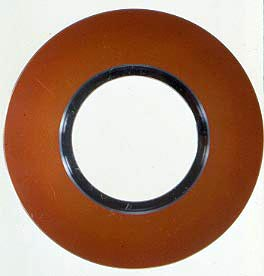
\includegraphics[width=5cm]{figs/magnetic_disk.jpg}}
        \label{FIG:MAGNETIC_DISK}

    \qquad
        \subfigure[b][Cart�o CCROS, adaptada de \cite{Richards:1965}]{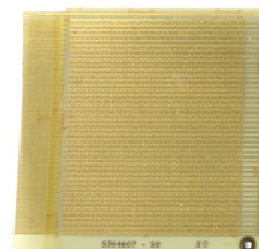
\includegraphics[width=5cm]{figs/ccros.jpg}}
        \label{FIG:Card_CCROS}
    \qquad
       \subfigure[c][Matriz de N�cleos de Mem�ria,  adaptada de \cite{Rent:2010}]{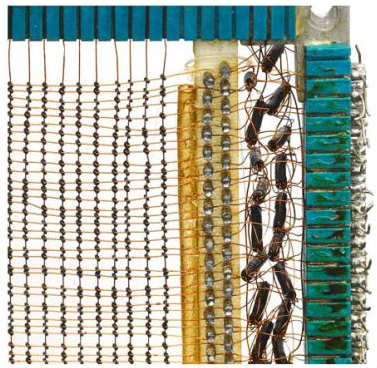
\includegraphics[width=5cm]{figs/ferritecore_small.png}}
        \label{FIG:CORE_MEMORY}
    \caption{Primeiros Dispositivos de Armazenamento}
\end{figure}


\subsection{Primeiros Dispositivos}

O primeiro equipamento a utilizar um \ac{DASD} n�o vol�til foi o \ac{RAMAC}, lan�ado pela \ac{IBM} em 1956. A unidade de disco do \ac{RAMAC}, chamada IBM 350, mostrada na Figura \ref{FIG:IBM350}, continha 50 discos, cada um com 24 $in$ de di�metro e que podiam armazenar 5 MB a uma densidade de grava��o de 2$Kbits/in^{2}$ \cite{Stevens:1981} e taxa de transfer�ncia de dados de $8.8 KB/s$\cite{Harker:1981}. Ela n�o possu�a sistema de controle de malha fechada para posicionamento da cabe�a de leitura e escrita.%151, Explicar malha fechada?

Em 1961, o primeiro dispositivo \ac{HDD} a usar de rolamentos de ar, \ac{ABS},\cite{Strom:2007}, foi lan�ado e, em 1963, o primeiro disco remov�vel.

Em 1964, o primeiro equipamento a utilizar cart�es \ac{CCROS}\footnote{Cart�es CCROS foram os primeiro dispositivos \ac{SSD}}, � lan�ado pela \ac{IBM}, era a fam�lia IBM System 360, fam�lia de \emph{mainframes}.\footnote{Mainframe, computador de grande porte, dedicado normalmente ao processamento de um volume grande de informa��es. }

Em 1971, a \ac{IBM} lan�ou o primeiro \ac{HDD} com controle de malha fechada, o IBM 330 \emph{Merlin Drive}. Ele mantinha a posi��o da cabe�a relativa � trilha do disco monitorada por um sensor de movimento.

Em 1973, a IBM introduziu outro modelo de \ac{HDD}, o IBM 3340, que usava cabe�a e bra�o de ferrite. Ele continha  2 ou 4 discos de 14 $in$ de di�metro, aproximadamente $35,56 cm$, possu�a capacidade de armazenamento de 35 MB para um dispositivos com 2 discos, taxa de transfer�ncia de dados de 0.8MB/s e densidade de grava��o m�dia de $1,69 Mbits/in^{2}$. Este ficou conhecido como disco Winchester, o primeiro \ac{HDD} a usar a malha de controle dos dispositivos atuais. % servo control loop.
 % Falar da IBM e da ahjuda dela
  \begin{figure}[htb]
  \centering
  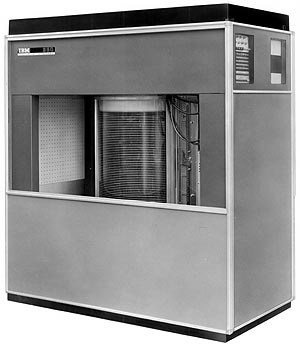
\includegraphics[scale=0.5]{figs/ibm350.jpg}
  \caption{IBM 350, adaptada de \cite{Morimoto:2007}}
  \label{FIG:IBM350}
\end{figure}


\subsection{Desenvolvimento dos \emph{Desktops}}

 O desenvolvimento de computadores \emph{desktop}, no in�cio da d�cada de 1980, representou uma nova era da tecnologia da informa��o. Este tipo de computador iniciou uma nova demanda na ind�stria de armazenamento de dados, pois os \acp{HD}, at� ent�o usados apenas para solu��es corporativas, teriam de se adequar a equipamentos mais compactos.

 A necessidade de \ac{DASD} com tamanho f�sico adequado a desktops se tornou evidente e foi quando os discos de $5\frac{1}{4}$ $in$ surgiram. Estes dispositivos tinham 5 MB de capacidade de armazenamento e traziam a primeira interface de disco, eram os discos da s�rie ST506, introduzida pela empresa Seagate Technology.

 A s�rie ST506 usava motor de passo como atuador. Esse motor, ao receber um impulso el�trico, movimenta o bra�o por uma curta dist�ncia, correspondente ao comprimento de uma trilha. Eles eram muito suscet�veis a problemas de desalinhamento e n�o permitiam densidades de grava��o muito altas. Logo nos primeiros anos da d�cada de 1980, foi produzido em grande escala o primeiro dispositivo de $5\frac{1}{4}$ $in$ com atuador do tipo \ac{VCM}\footnote{Motores Voice Coil s�o atuadores cujo funcionamento baseia no de um alto-falante, onde uma bobina � excitada por corrente (sinal de �udio), e um �m� permanente interage com o campo dessa bobina, deslocando um cone e produzindo ondas mec�nicas de som.}, dispositivo que atua atrav�s de atra��o e repuls�o magn�tica. %Apesar de o motor de passo continuar presente por mais alguns anos.

 Em 1983, o primeiro \ac{HDD} com discos de $3\frac{1}{2}$ $in$ de di�metro foi lan�ado pela empresa Rodime.

 At� ent�o, n�o havia interfaces de disco padronizadas e as novas interfaces eram vendidas junto com os \acp{HD} e instaladas em slots \ac{ISA} dispon�veis na placa-m�e, \cite{Morimoto:2007}. Em 1985 a Quantum Corporation lan�ou o \emph{Plus HardCard}, em que tanto a controladora quanto o \ac{HD} eram integrados em um �nico slot \ac{ISA}. Esta integra��o se mostrou vantajosa pois diminu�a problemas de sincronismo e simplificava o projeto, e isto deu origem ao padr�o \ac{IDE}.

 Apenas em 1990 o padr�o \ac{IDE} foi ratificado pelo \ac{ANSI}, organiza��o que tem por objetivo facilitar a padroniza��o dos trabalhos de seus membros, dando origem ao padr�o \ac{ATA}.

  Nos anos seguintes, os \acp{HD} de $5\frac{1}{4}$ $in$ come�aram a perder mercado para os \acp{HD} de $3\frac{1}{2}$ $in$ e $2\frac{1}{2}$ $in$, posteriormente usados no mercado de laptops. Estes formatos foram bem aceitos pelo mercado, sendo utilizados at� hoje.

 Paralelamente a estes avan�os, o desenvolvimento de mem�rias \emph{Flash} come�ava a dar os primeiros passos. As mem�rias \emph{Flash} foram desenvolvidas a partir das mem�rias \ac{EEPROM}. Em 1984, o Dr. Masuoka publicou sua inven��o no artigo ``\emph{A New Flash EEPROM  Cell Using Triple Polysilicon Technology} '' \cite{Masuoka:1984}.

  Em 1987, a Toshiba anuncia as mem�rias \emph{Flash} do tipo \emph{NAND} e em 1988 a Intel anuncia as mem�rias \emph{Flash} do tipo \emph{Nor}, \cite{Bez:2003}. Hoje, estes dois tipos s�o considerados os padr�es da ind�stria. A mem�ria \emph{Flash} do tipo \emph{Nand} � otimizada para o armazenamento de dados em massa e a do tipo \emph{Nor} para o armazenamento de dados e c�digo\footnote{\emph{Flash} do tipo \emph{Nor} s�o usadas para armazenar informa��es na BIOS da placa-m�e e \emph{firmwares} em dispositivos diversos, pois, embora requeiram pouco tempo para a leitura, apresentam um tempo de grava��o alto.}.  Em 1988, o primeiro produto \emph{Flash} foi apresentado \cite{Kunnet:1988}, tratava-se de um \emph{chip} de mem�ria \emph{Flash} do tipo \emph{Nor} de 256KB.

  Inicialmente, as mem�rias \emph{Flash} foram usadas para a substitui��o de mem�rias EPROM \footnote{EPROM,\emph{Erasable Programmable Read-Only Memory}} \cite{Bez:2003} e s� passaram  a ser utilizadas em larga escala no final dos anos 1990.
   %% checar isso
   Os primeiros \acp{HD} \ac{SSD} baseados em \emph{Flash} s� chegaram ao mercado em 2007.

\section{Padr�es Adotados}
 Com o passar dos anos, v�rias empresas come�aram a fabricar discos r�gidos e, visando a compatibilidade entre diferentes discos r�gidos e computadores, padr�es de tamanho e de interfaces foram adotados.

\subsection{\emph{Form Factors}}
 Os discos r�gidos foram projetados para serem instalados dentro de computadores, e s�o produzidos em poucos padr�es de tamanho e forma. Estes padr�es s�o chamados de \emph{form factors} de discos r�gidos, algo como configura��es padr�o, e se referem principalmente �s dimens�es externas dos discos r�gidos, \cite{Mamun:2007}.

 A Figura \ref{FIG:Form_Factor},  mostra seis \acp{HDD} com as tampas removidas deixando � mostra os \emph{platters} e as cabe�as, onde os padr�es de discos de 8, 5.25, 3.5, 2.5, 1.8 e 1 $in$ de di�metro s�o representados.

Nos \acp{HDD}, os \emph{form factors} geralmente s�o limitados pelo tamanho do disco e os \acp{SSD}, embora  n�o tenham esta limita��o, geralmente seguem o mesmo padr�o para serem compat�veis com as estruturas existentes em \emph{laptops} e \emph{desktops}.

\begin{figure}[htb]
  % Requires \usepackage{graphicx}
  \centering
  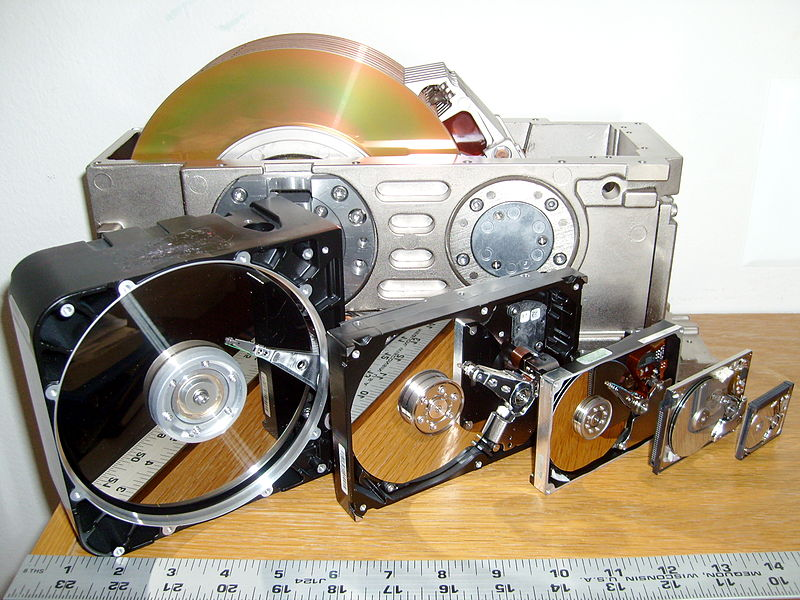
\includegraphics[scale =0.45]{figs/form_factors.jpg}\\
  \caption{ Seis configura��es padr�o de Discos R�gidos,  adaptada de \cite{Potts:2008}}\label{FIG:Form_Factor}
\end{figure}

\subsection{Interfaces}
Da mesma forma que outros componentes dos \acp{HD}, as interfaces que os interligam passaram por muitas mudan�as.
Atualmente existem dois tipos predominantes no mercado: ATA e SCSI, ambas s�o padr�es \ac{ANSI}. Estes padr�es definem conectores, conex�es f�sicas, como sinais e temporiza��o, protocolos de transporte, modelos de dispositivos e comandos. Estes modelos e comandos s�o a base do desenvolvimento do \emph{Framework} proposto neste trabalho e ser�o detalhados no Cap�tulo \ref{CHP:TEO}.

O padr�o \ac{ATA}, tamb�m conhecido como \ac{IDE}, foi projetado para ser uma interface entre computadores e discos r�gidos.
 Diversas vers�es foram definidas at� agora, s�o elas: \ac{ATA} 1 ou \ac{IDE}, \ac{ATA} 2 ou \ac{EIDE}, \ac{ATA} 3, \ac{ATA}$\backslash$\ac{ATAPI} 4, \ac{ATA}$\backslash$\ac{ATAPI} 5, \ac{ATA}$\backslash$\ac{ATAPI} 6, \ac{ATA}$\backslash$\ac{ATAPI} 7 e \ac{ATA}$\backslash$\ac{ATAPI} 8.

 A vers�o \ac{ATA} 3 foi a primeira a trazer o sistema \ac{SMART} e, a partir da vers�o \ac{ATA} 4, o padr�o \ac{ATA} se tornou capaz de enviar comandos \ac{SCSI} encapsulados em comandos \ac{ATA}, possibilitando a comunica��o com outros perif�ricos como unidades de discos �pticos. Esta extens�o do protocolo \ac{ATA} foi chamada de \acf{ATAPI}.

O padr�o \ac{SCSI} foi desenvolvido para ser um padr�o gen�rico para perif�ricos, como \emph{scanners}, unidades de discos �pticos, m�dias remov�veis e discos r�gidos. Ele foi padronizado pela \ac{ANSI} em 1986 e dele foram desenvolvidas as seguintes vers�es: \ac{SCSI} 1, \ac{SCSI} 2, com suporte a comandos \emph{multi-thread}, e \ac{SCSI} 3, com separa��o entre conex�o f�sica, protocolos de transporte e conjuntos de comandos \ac{SCSI}.

O \ac{SCSI} oferece  melhor desempenho que o \ac{ATA} em aplica��es que requerem velocidade de processamento e transfer�ncia de grande quantidades de dados \cite{Mason:2000}, por isso os discos \ac{SCSI} s�o tipicamente mais caros e, em geral, usados em servidores, onde o alto custo � justific�vel. J� os discos \ac{ATA} s�o mais utilizados em computadores pessoais.

Os computadores se tornaram mais r�pidos e as interfaces precisavam atender a esta demanda e, neste intuito, tanto o padr�o \ac{ATA} quanto o \ac{SCSI}, antes interfaces paralelas, tenderam � serializa��o, utilizando pares diferenciais, visando alcan�ar maiores velocidades de transmiss�o e evitar problemas de interfer�ncia entre as vias. Desta iniciativa surgiram os padr�es \ac{SATA} e \ac{SAS}, protocolos seriais de transporte e interconex�o f�sica das interfaces \ac{ATA} e \ac{SCSI}, respectivamente, e as interfaces anteriores passaram a ser chamadas de \ac{PATA} e \ac{SPI}.

\section{\emph{Hard Disk Drive}}

De maneira resumida os \acp{HDD} s�o a integra��o dos seguintes componentes, descritos na Figura \ref{FIG:COMPHDD}:
\begin{itemize}
  \item Discos magn�ticos (\emph{platters}\footnote{\emph{Platters} s�o discos magn�ticos compostos por duas camadas, o substrato, um disco feito de liga de alum�nio ou vidro, extremamente polidos para tentar evitar qualquer rugosidade, e a superf�cie magn�tica, que possui apenas alguns micr�metros de espessura \cite{Morimoto:2007}. Neles cada bit � armazenado em um setor de fino segmento destas superf�cies atrav�s da magnetiza��o do meio pela cabe�a de grava��o.}), onde os dados s�o armazenados;
  \item Motor de rota��o, respons�vel por girar os \emph{platters} a uma velocidade angular constante adequada � leitura e grava��o de dados;
  \item Pares de cabe�as de leitura e escrita de dados (h� duas para cada lado de um \emph{platter});
  \item Bra�o met�lico, onde se encontram as cabe�as de leitura e escrita;
  \item Atuador, mecanismo composto por um motor \ac{VCM} e pelo bra�o met�lico;
  \item Conector, atualmente a maioria s�o do tipo \ac{SATA} ou \ac{SAS};
  \item Placa controladora \ac{PCB}, que � respons�vel por acionar o motor que gira os \emph{platters}, posicionar as cabe�as de leitura e escrita, atrav�s do atuador, e executar os comandos recebidos pelo sistema atrav�s de um conector, tais comandos podem ser \ac{ATA} ou \ac{SCSI}. A placa controladora pode ser interna, como nos discos \ac{SATA}, ou externa, como nos discos \ac{SCSI}, \cite{Carrier:2005file}.

\end{itemize}

% Inserir tabela aqui

\begin{figure}[htb]
  \centering
  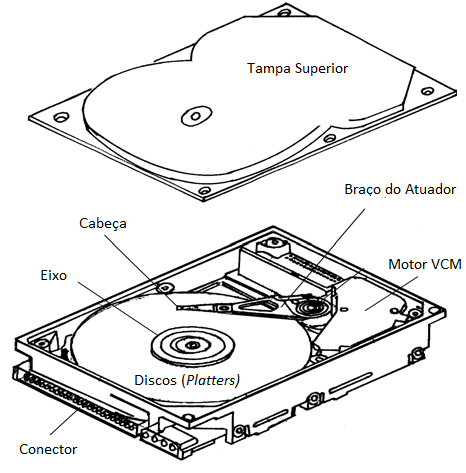
\includegraphics[scale=0.8]{figs/componenteshdd.png}
  \caption{Componentes normalmente encontrados em HDDs, adaptada de \cite{Mamun:2007} }
  \label{FIG:COMPHDD}
\end{figure}

Ao contr�rio do que se possa pensar, o \ac{HDD} n�o � vedado ou blindado. Seu funcionamento se baseia em aerodin�mica. As cabe�as n�o devem entrar em contato com os \emph{platters}, pois isso os danificaria e por isso eles s�o girados a uma alta velocidade de rota��o e s� ent�o o bra�o � movimentado, isto gera uma ``bolsa'' de ar, uma folga entre a cabe�a e os \emph{platters}\footnote{Esta folga � chamada de \emph{Head-Disk Clearance}, \cite{Strom:2007}}, fazendo com que as cabe�as flutuem\footnote{Esta bolsa de ar criada funciona como rolamento de ar, o sistema \ac{ABS} descrito anteriormente} sobre eles. Esta folga pode ser alterada por par�metros ambientais como a temperatura, a press�o atmosf�rica e a umidade do ar \cite{Strom:2007}.

Nos \acp{HDD} existem uma entrada de ar que passa por um filtro, antes de  entrar em contato com os \emph{platters}. Embora n�o seja blindado, abrir um \ac{HDD} fora de uma  sala limpa\footnote{Sala Limpa, ambiente controlado utilizado para testes ou manufatura de produtos onde a contamina��o por part�culas presentes no ar interfere no resultado} pode acarretar na inutiliza��o do mesmo, pois qualquer part�cula de poeira presente no ambiente poderia danificar a superf�cie dos \emph{platters} \cite{Zhao:2007}.

Os \acp{HDD} atuais cont�m normalmente de 1 a 4 \emph{platters} e, para cada lado de um \emph{platter}, h� duas cabe�as acopladas, uma de escrita e outra de leitura. Elas est�o presas por espa�adores ao bra�o e embora haja um conjunto de cabe�as para cada lado do \emph{platter}, elas n�o s�o independentes. Todas se movimentam como uma s�, guiadas pelo bra�o, como mostrado na Figura \ref{FIG:Discos_Cabe�a_Bra�os}.a. Os \emph{platters} s�o organizados em trilhas conc�ntricas e estas trilhas organizadas em setores, como mostrado na Figura \ref{FIG:Trilhas_setores}.b.

\begin{figure}[htb]
    \centering
    \subfigure[a][Discos, bra�o e cabe�as de um \ac{HDD}, adaptada de \cite{Vasconcelos:2002}]{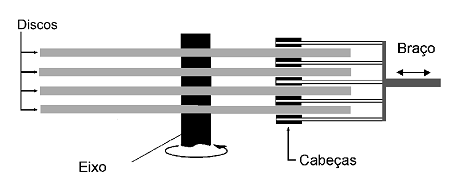
\includegraphics[width=8cm]{figs/discos_cabecas_braco.png}}
        \label{FIG:Discos_Cabe�a_Bra�os}
    \subfigure[b][Trilhas e setores, adaptada de \cite{Vasconcelos:2002} ]{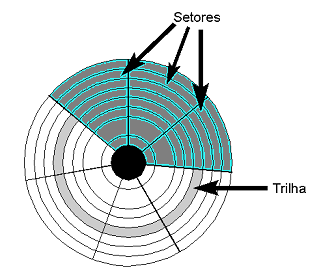
\includegraphics[width=5cm]{figs/trilhas_setores.png}}
        \label{FIG:Trilhas_setores}
    \caption{Componentes de um \ac{HDD}}
\end{figure}

\section{\emph{Solid-State Drive}}
Os Solid-State Drives (\ac{SSD}) podem ser definidos como dispositivos que armazenam dados em \emph{chips}, na maioria dos casos mem�rias \emph{Flash}, e sem partes mec�nicas, como mostrado na Figura \ref{FIG:SSD}.

\begin{figure}[!htb]
  \centering
  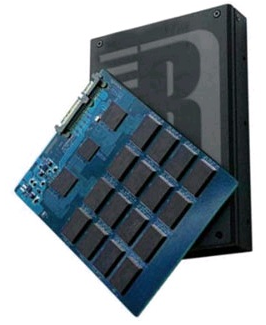
\includegraphics[width=6cm]{figs/ssd.png}
  \caption{Solid-State Drive, adaptada de \cite{Happy:ssd}}
  \label{FIG:SSD}
\end{figure}

Os principais componentes de um \ac{SSD} s�o a controladora, os m�dulos de mem�ria \emph{cache}, do tipo \ac{DRAM}, e mem�ria \emph{Flash}, normalmente 10 ou 20, e o conector, que pode ser do tipo \ac{SATA}, \ac{SAS}, entre outros \cite{Rent:20102}, como mostrado na Figura \ref{FIG:SSD_comp}.

\begin{figure}[!htb]
  \centering
  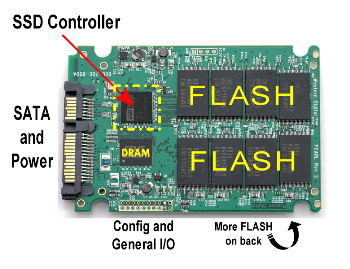
\includegraphics[width=8cm]{figs/ssd_controller.png}
  \caption{Componentes de um SSD, adaptada de \cite{Rent:20103}}
  \label{FIG:SSD_comp}
\end{figure}

 A controladora, cuja a estrutura � mostrada na Figura \ref{FIG:SSD_controller}, consiste de um processador embarcado, normalmente um microcontrolador de 32 \emph{bits}, que executa c�digo em n�vel de \emph{firmware}, como o \ac{SMART}, gerencia automaticamente a mem�ria\footnote{\emph{Garbage Collector}} e executa  comandos, como o comando TRIM\footnote{TRIM � um comando \ac{ATA} para gerenciamento de dados, respons�vel por informar quais blocos de dados n�o est�o mais em uso,\cite{Intel:2010}.}, por exemplo. Ela tamb�m gerencia as mem�rias DRAM, ROM e interfaces de entrada e sa�da existentes no \ac{SSD}.

\begin{figure}[!htb]
  \centering
  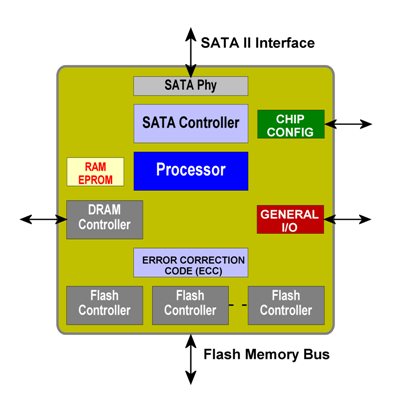
\includegraphics[width=8cm]{figs/ssd_controller_elements.png}
  \caption{Controladora de um SSD, adaptada de \cite{Rent:20103}}
  \label{FIG:SSD_controller}
\end{figure}

Nos \acp{SSD} o espa�o de armazenamento  � dividido em blocos de dados, em geral de 512KB, e estes blocos em p�ginas, usualmente  de 4KB. O espa�o � preenchido primeiramente sem repetir escritas nos setores, depois que todos os setores s�o preenchidos.
%http://www.infowester.com/ssd.php

\section{\emph{Hard Disk Drive} versus \emph{Solid-State Drive } }

Os \acp{HDD} e \acp{SSD} utilizam as mesmas interfaces, possuem controladora, seja ela interna ou externa, organiza��o dos dados em setores, c�digos de corre��o de erro, endere�amento por \ac{LBA}\footnote{Os primeiros \acp{HDD} utilizavam endere�amento baseado no espa�o f�sico, o \ac{CHS}, que identificava um setor pelo cilindro, cabe�a e posi��o na trilha em que estava, mas este modo de endere�amento era limitado pela \ac{BIOS} e foi substituido pelo \ac{LBA}, baseado na representa��o l�gica dos setores. } e �rea reservada de mem�ria (\emph{spare area}). No entanto, as duas tecnologias usam princ�pios de armazenamento diferentes, e h� muitas diferen�as de desempenho e de fontes de falha.

\subsection{Desempenho}
Em compara��o aos \acp{HDD}, os \acp{SSD} s�o menos afetados por choques f�sicos, pois n�o cont�m partes m�veis, s�o mais silenciosos e t�m menor consumo de energia el�trica. %e tempo de acesso e lat�ncia. A lat�ncia se refere ao tempo de espera antes do setor desejado para escrita ou leitura estar pronto. E o tempo de acesso se refere � soma da lat�ncia m�dia e do tempo de busca, tempo necess�rio para posicionar o bra�o do \ac{HDD}.

Os \acp{SSD} t�m um tempo de inicializa��o menor, s�o mais r�pidos na escrita e leitura aleat�ria e na leitura sequencial de arquivos grandes. Na Figura \ref{FIG:benchmark}, um \emph{benchmark}\footnote{Execu��o s�ries de testes e ensaios visando avaliar o desempenho relativo de um produto} � mostrado entre \acp{HDD} de 7200 rpm e 5400 rpm e um \ac{SSD} Toshiba MLC NAND\footnote{O \emph{Benchmark} foi realizado usando processador Intel Core2Duo 2.2GHz E4500, mem�ria cache L2 de 2MB, mem�ria RAM de 2GB DDR SDRAM com 800MHz, placa gr�fica Intel GMA3100 e sistema operacional Windows$\circledR$ Vista}. Nele, o dispositivo \ac{SSD} apresenta resultados bem superiores em termos de taxa de transfer�ncia de dados, especialmente na inicializa��o de aplica��es. Entretanto, os \emph{chips} de mem�ria \emph{flash}, usados nos \acp{SSD}, tem limites de regrava��o estimados em 10.000 vezes, se forem do tipo \ac{MLC}, ou 100.000, se forem do tipo \ac{SLC} \cite{Morimoto:2010}, o que compromete a sua longevidade, enquanto que nos \acp{HDD}, a quantidade de escritas est� associada apenas ao desgaste do material ou a danos f�sicos.

\begin{figure}[!htb]
  \centering
  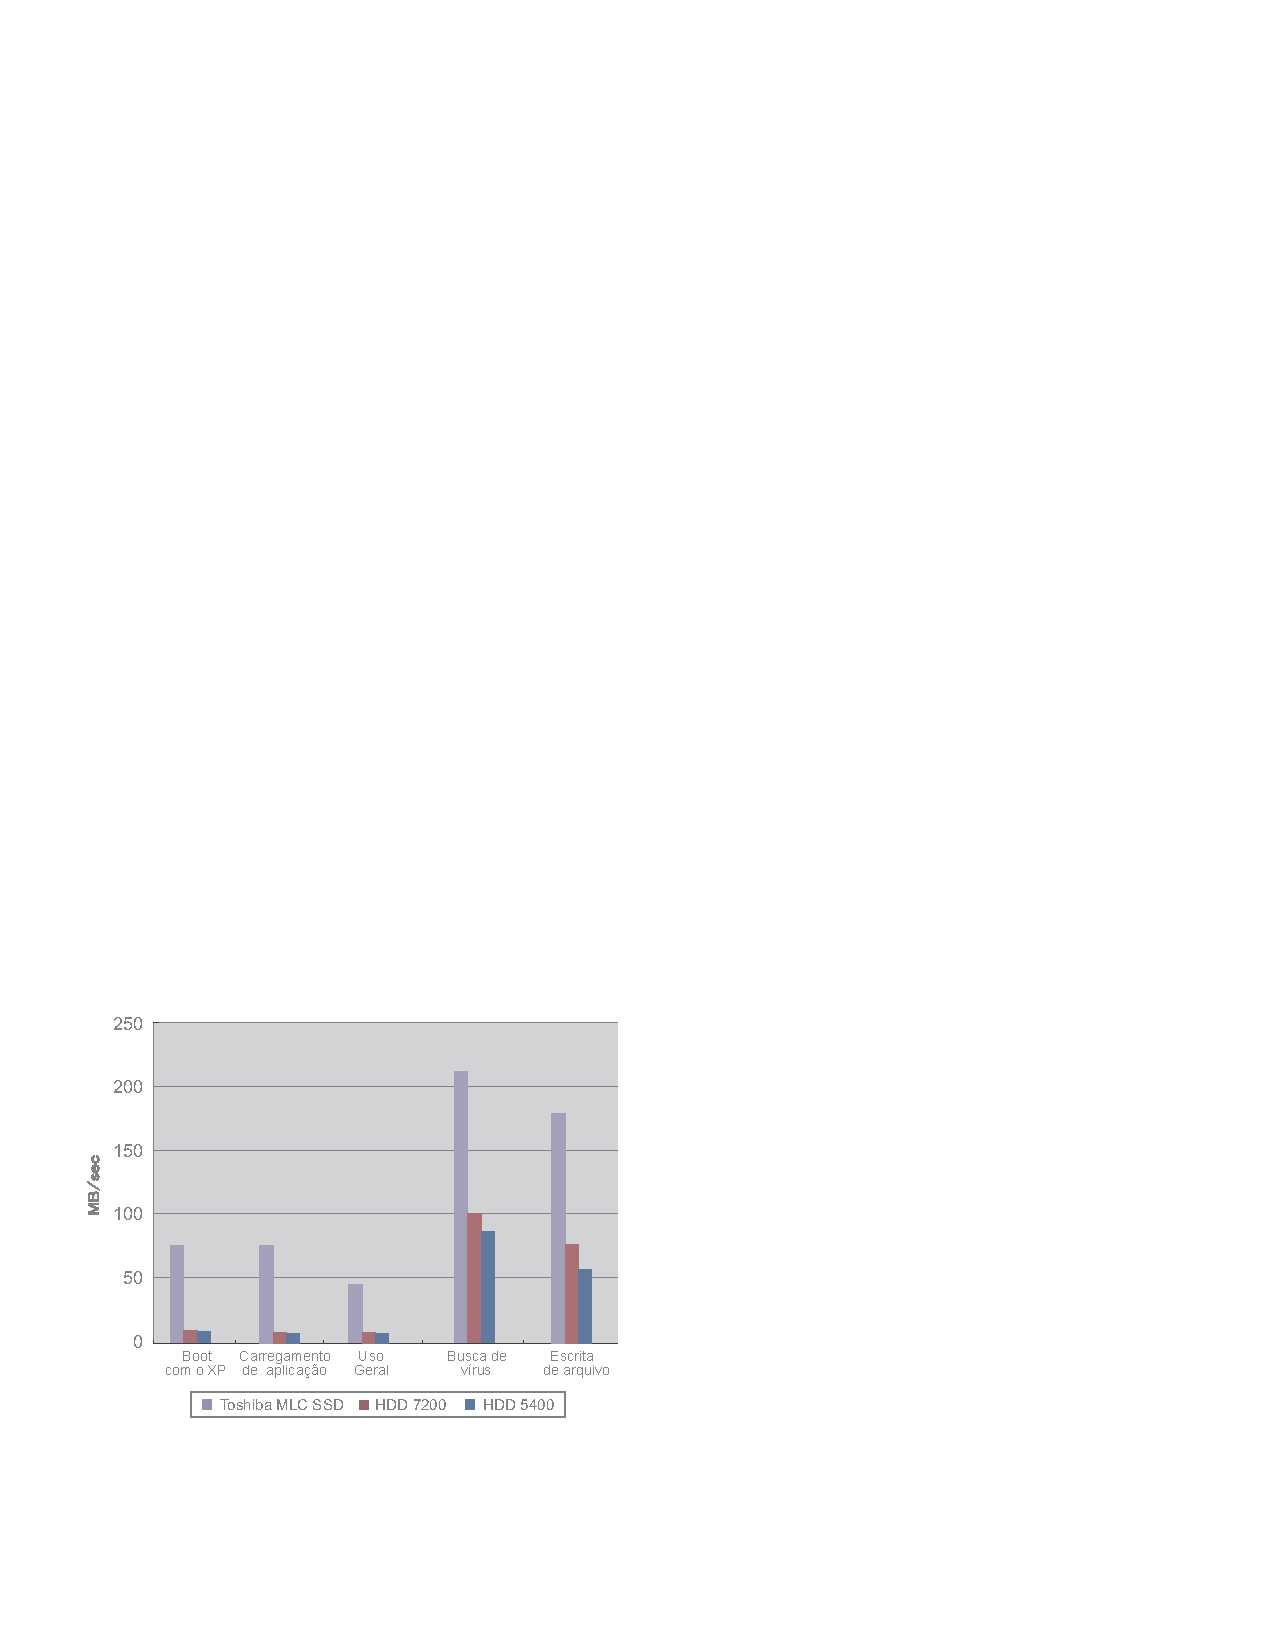
\includegraphics[width=11cm]{figs/benchmark.pdf}
  \caption{\emph{Benchmark} realizado pela PCmark05, adaptada de \cite{Toshiba:2010}}
  \label{FIG:benchmark}
\end{figure}



A capacidade de armazenamento e o custo por GB tamb�m s�o pontos que diferem nas duas tecnologias. At� setembro de 2011, o dispositivo \ac{SSD} de maior capacidade tinha 1.6 TB, \emph{form factor} de $2.5 in$ , e o \ac{HDD} de maior capacidade possu�a 4TB, \emph{form factor} de 3.5 $in$. O custo por GB, no dispositivo \ac{HDD}, era de 0,0625 d�lares \cite{Parrish:2011} e o  do dispositivo \ac{SSD}, embora n�o tivesse o pre�o anunciado, estimava-se um custo por GB superior a 6 d�lares, que �  custo por GB de um \ac{SSD} de 1 TB \cite{SHimpo}, o segundo maior dispositivo do tipo. Nestes quesitos, os dispositivos \ac{HDD}, com custos quase 100 vezes menores, s�o bastante superiores e sua predomin�ncia no mercado � justificada.


\section{Resumo do Cap�tulo}

Este cap�tulo mostrou um pouco da hist�ria dos discos r�gidos, os principais padr�es, a evolu��o das tecnologias \ac{SSD} e \ac{HDD} e um comparativo entre elas.

No pr�ximo capitulo ser�o abordados fundamentos de diagn�stico de falha, o sistema \ac{SMART}, e as principais caracter�sticas dos padr�es \ac{ATA} e \ac{SCSI}.

%%%% CAP�TULO 3: Ferramentas de Diagn�stico
\chapter{Fundamenta��o Te�rica} \label{CHP:TEO}%%

Neste cap�tulo s�o explorados os alicerces deste trabalho: os fundamentos de diagn�stico de falha, os padr�es adotados em discos r�gidos e como interagir com eles atrav�s do Linux.

\section{Fundamentos de Diagn�stico de Falhas}

Primeiramente, para explicar o conceito deste trabalho, � necess�rio que se defina o conceito de falha, o conceito de diagn�stico e as origens das falhas no dispositivo em estudo, os discos r�gidos.

\subsection{Falha, Erro e Defeito}

Embora sejam usadas como sin�nimo, estas palavras tem significados diferentes para sistemas de computa��o. A falha est� associada ao universo f�sico, o erro � a representa��o da falha no universo da informa��o, � causado por uma falha, e o defeito � um desvio da especifica��o e ocorre em consequ�ncia de um erro \cite{lee1990fault}, as rela��es de causa entre elas est�o ilustradas na Figura \ref{FIG:falha_erro_defeito}.

Uma falha pode ser ocasionada por um problema em n�vel de \emph{hardware}, uma flutua��o de tens�o ou um impacto que cause uma avaria em  um setor de um disco r�gido, por exemplo, e n�o necessariamente leva a um estado de erro. O erro acontece quando uma informa��o � corrompida devido a um setor falho e tamb�m n�o necessariamente leva a um estado de defeito, que � detectado no n�vel de usu�rio, pois talvez a informa��o corrompida nunca seja usada, ou possa ser recuperada. % Ex: Hamming Reed Solomons


\begin{figure}[!htb]
  \centering
  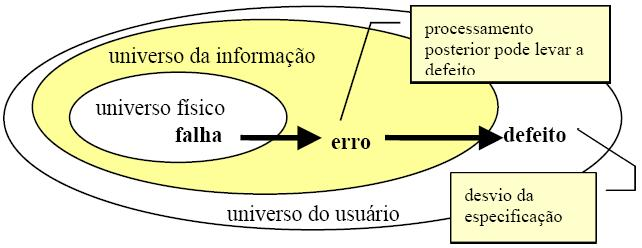
\includegraphics[width=10cm, angle=0]{figs/falha_erro_defeito.jpg}\\
  \caption{Modelo de tr�s universos, adaptada de \cite{Wesz:2007}}
 \label{FIG:falha_erro_defeito}
\end{figure}

\subsection{Diagn�stico de Falhas}

Com o prop�sito de evitar que um sistema se torne defeituoso, as falhas devem ser detectadas e diagnosticadas. A detec��o de falhas se baseia em sistemas te�ricos, modelos de processo ou fun��es matem�ticas para reconhecer sintomas de falha. Estes sintomas s�o desvios das caracter�sticas do processo modelado. O diagn�stico de falhas � diferente da detec��o de falhas, que consiste em reconhecer que uma falha aconteceu.

Diagnosticar falhas consiste na identifica��o do tipo de falha com a maior quantidade de detalhes poss�veis, bem como a extens�o da falha, localiza��o e o momento da detec��o \cite{Isermann:2011}. O procedimento de diagn�stico � baseado na observa��o e an�lise de sintomas e no conhecimento pr�vio sobre o processo. Os sintomas dispon�veis podem ser:

\begin{description}
  \item[Sintomas Anal�ticos.] S�o o resultado da compara��o entre os sinais de um processo e do seu modelo de detec��o de falha. Verifica-se se estes sinais excederam algum limiar pr�-determinado;
  \item[Sintomas Heur�sticos.] S�o resultado da an�lise de um operador humano. Trata-se de impress�es quanto a ru�do, oscila��es, cores e fuma�a obtidos por inspe��o. Tratados muitas vezes como medidas qualitativas;
  \item[Hist�rico de processos e estat�sticas de falha.] Este hist�rico inclui infor- ma��es sobre tempo de execu��o e reparo e descrevem a frequ�ncia de certas falhas no processo;
  \item[Representa��o unificada dos sintomas.] � a observa��o conjunta de sintomas anal�ticos e heur�sticos, atrav�s de mecanismos de infer�ncia de sistemas \emph{fuzzy};
  \item[Rela��es Falha-Sintomas.] Consistem na an�lise inversa das rela��es de causa e efeito. Na an�lise direta, observam-se falhas que geram eventos que geram sintomas. Na an�lise inversa, as falhas s�o deduzidas a partir dos sintomas observados;
\end{description}

\subsection{Falhas em Discos R�gidos}\label{falhashd}

Segundo \cite{Kari:1997}, as falhas em discos r�gidos podem ser ocasionadas por falhas no meio de armazenamento, que podem causar a perda de dados, ou por outras falhas como problemas de alimenta��o, problemas na controladora do disco ou software, por exemplo, e que n�o necessariamente causam a perda de dados, mas levam � sua indisponibilidade tempor�ria.

Os discos r�gidos s�o organizados em pequenos m�dulos de armazenamento, chamados de setores,  nos \acp{HDD}, ou blocos, nos \acp{SSD}. Aqui estes m�dulos ser�o chamados genericamente de setores. Estes setores disp�em das seguintes informa��es: identifica��o, usada para localizar o setor, como \ac{LBA}, por exemplo; dados, a informa��o em si; campos de sincroniza��o, usados internamente pela controladora para guiar o processo de leitura; espa�adores (\emph{Gaps}), usados  para separar setores e dar tempo para que a controladora processe o que estava sendo lido; e c�digos de corre��o de erro, como \ac{CRC}, por exemplo \cite{Sector:2001}, que s�o usados pela controladora para detectar a ocorr�ncia de falhas.

As falhas em discos r�gidos podem ser divididas quanto � dura��o, como tempor�rias ou permanente; e quanto � magnitude, como parcial, intermedi�ria  ou total \cite{Kari:1997}. Falhas tempor�rias podem ser causadas por mudan�as de estado do sistema. Um exemplo de situa��o de falha tempor�ria � quando um comando n�o � completado com sucesso e atrav�s da repeti��o ele pode ser completado sem erros. Falhas permanentes s�o duradouras, mas os erros causados por elas talvez possam ser contornados por c�digos de corre��o de erro ou leitura de outros setores, por exemplo. Em rela��o � magnitude, uma falha pode afetar todo o disco ou uma pequena parte dele. Normalmente, um setor � a m�nima �rea afetada.

As falhas podem ser geradas no processo de fabrica��o. Alguns \acp{HD} novos j� saem de f�brica com setores falhos\footnote{Em ingl�s \emph{Bad blocks} ou \emph{Bad sectors}} e outros setores se danificam em decorr�ncia do uso e desgaste natural. Os setores falhos s�o remapeados em uma �rea reservada. Enquanto que nos \acp{HDD} isto pode gerar perda de desempenho, pois gera mais movimentos de busca para ler um arquivo, por exemplo, nos \acp{SSD} este mapeamento � praticamente transparente. A �rea reservada  tem duas fun��es principais: servir de armazenamento tempor�rio de novos dados e ser uma esp�cie de mem�ria ``reserva'' , onde os setores com falha s�o remapeados, aumentando a longevidade do disco r�gido \cite{Morimoto:20102}.

 A �rea reservada � gerenciada pela controladora e se relaciona com a diferen�a entre a nomenclatura decimal utilizada pelos fabricantes e a nomenclatura bin�ria usada pelos sistema operacional. Por exemplo, cada 1GB de mem�ria na nomenclatura do fabricante corresponde a $10^9$ \emph{bytes}, o que para um sistema operacional corresponde a $2^{30}$ \emph{bytes} e a diferen�a entre as duas nota��es, igual a 73.741.824 \emph{bytes}, � a quantidade de mem�ria a ser usada como �rea reservada.

O remapeamento de setores com falha � transparente para o sistema operacional. Quando um setor falho � requisitado, a controladora intercepta e devolve o dado correto do novo bloco atribu�do �quele endere�o na �rea reservada. Apenas quando esta �rea est� totalmente cheia, o sistema operacional come�a a indicar a exist�ncia de setores falhos.

Nos \acp{SSD} os tipos mais comuns de falha em c�lulas de mem�ria est�o relacionados a dist�rbios de grava��o, problemas na reten��o de dados e defeitos de fabrica��o. Cada c�lula armazena um bit de mem�ria. Os dist�rbios de grava��o consistem na corrup��o de dados de c�lulas escritas durante a escrita de outras c�lulas na mesma matriz de mem�ria \cite{Bez:2003}. Estes dist�rbios podem acontecer nas c�lulas de mesma coluna ou linha.

Nos \acp{HDD}, assim como nos \acp{SSD}, existem dist�rbios de grava��o, problemas na reten��o de dados e defeitos de fabrica��o. Os dist�rbios de grava��o podem ocorrer entre setores adjacentes, trilhas vizinhas e at� mesmo entre \emph{platters}, j� que h� um movimento unificado � todas as cabe�as. Um exemplo de dist�rbio de grava��o � a propaga��o radial do erro \cite{Zhao:2007}, onde, por algum motivo, uma trilha n�o � escrita como um c�rculo perfeito\footnote{Este fen�meno � chamado \emph{track misregistration} (TMR)} e, quando esta � referenciada para leitura, a cabe�a segue um c�rculo perfeito assim como para as trilhas seguintes, onde os setores desejados n�o est�o e outros setores s�o lidos.

Al�m das falhas originadas pelo desgastes ou defeitos de fabrica��o do meio magn�tico, os \acp{HDD} podem apresentar v�rias fontes de falhas inseridas pelas partes m�veis  assim como por fatores ambientais e impactos f�sicos. Por exemplo, quando uma tentativa de leitura de um setor falha, a causa tanto pode ser um dist�rbio de grava��o, quanto uma falha no atuador, que n�o conseguiu posicionar a cabe�a corretamente. Outro exemplo � a folga existente entre as cabe�as e os \emph{platters}, que diminui com o aumento da temperatura, com a diminui��o da press�o atmosf�rica, e tamb�m com o aumento da humidade do ar. Esta diminui��o da folga pode levar ao choque das cabe�as com pontos de maior rugosidade nos \emph{platters} e estes choques podem gerar erros de leitura e grava��o e danificar o disco r�gido.

H� dois meios de detectar setores falhos em discos r�gidos: atrav�s de requisi��es normais do sistema operacional, leituras e escritas, e atrav�s de buscas, como execu��es de  algoritmos de testes, por exemplo. Segundo \cite{Kari:1997}, as falhas em discos r�gidos est�o fortemente relacionadas umas com as outras, ou seja, a probabilidade de um setor falhar � significativamente maior em �reas pr�ximas �s regi�es de falhas conhecidas. Falhas tempor�rias s�o o primeiro sinal de deteriora��o do meio e podem ser usadas para predizer falhas permanentes. Estas informa��es podem ser utilizadas no desenvolvimento de algoritmos de teste.
%\example{Listagem deu Certo.}

\section{SMART}

A ind�stria de \acp{HD} adotou um sistema de monitoramento para discos r�gidos, o sistema \acs{SMART}, visando detectar falhas, disponibilizar diferentes tipo de auto-teste e relatar medidas indicadoras de confiabilidade. O \ac{SMART}  prev� falhas em discos r�gidos individualmente, diferentemente dos modelos de confiabilidade, que depois de an�lises estat�sticas calculam a probabilidade de falha de uma popula��o de discos r�gidos, supondo que todos s�o iguais. O \ac{SMART} prev� falhas atrav�s de medidas e contagens, como a quantidade de setores realocados, taxa de erro de leitura, a quantidade de choques f�sicos sofridos e o tempo total de uso, por exemplo.  Na Tabela \ref{TAB:smart} alguns atributos monitorados pelo \ac{SMART} s�o mostrados.

\begin{table}[htb!]
    \begin{center}
    \label{TAB:smart}\caption{Exemplos de atributos \ac{SMART} para \ac{ATA}}
    \vspace{-10pt}
    %\centering
        \begin{tabular}{|c|p{6 cm}|p{6 cm}|}
         \hline
         % after \\: \hline or \cline{col1-col2} \cline{col3-col4} ...
         Identificador & Atributo  & Descri��o  \\ \hline
         01 & Taxa de erro de leitura (\emph{Read Error Rate}) & Frequ�ncia de erros durante a leitura de dados do disco. \\ \hline
         02 & Desempenho (\emph{Throughput Performance}) & Efici�ncia m�dia do disco. \\ \hline
         05 & Contagem de setores realocados (\emph{Reallocated Sectors Count}) & Contagem dos setores realocados na �rea reservada. \\ \hline
         08 & Desempenho das opera��es de busca (\emph{Seek Time Performance}) & Desempenho m�dio das opera��es de busca nos discos magn�ticos. A diminui��o deste atributo pode indicar problemas no sistema mec�nico. \\ \hline
         191 & Taxa de erro devido a impactos (\emph{G-sense Error Rate})& Frequ�ncia de erros resultantes de impactos e vibra��es. \\ \hline
         194 & Temperatura (\emph{Temperature}) & Temperatura interna do disco. \\ \hline
         197 & Contagem atual de setores pendentes (\emph{Current Pending Sector Count}) & N�mero de setores esperando para serem remapeados. \\ \hline
        \end{tabular}
    \end{center}
    \vspace{-15pt}
\end{table}

Um algoritmo de alerta de falha � executado pelo \emph{firmware} da controladora do disco r�gido e checa se as medidas excederam o limiar m�ximo e gera um alerta bin�rio do tipo: Ir� falhar, N�o Ir� Falhar. Os limiares m�ximos s�o definidos pelos fabricantes. O objetivo � gerar o alerta 24 horas antes de o \emph{drive} falhar, \cite{Hughes:2002}.

H� comandos padronizados para habilita��o e leitura desses alertas de falha pelos sistemas operacionais. Alguns computadores checam o \ac{SMART} durante a inicializa��o do sistema operacional e alguns fabricantes disponibilizam programas de diagn�stico que l�em os alertas do \ac{SMART} \cite{Hughes:2002}. O sistema \ac{SMART} foi especificado para o padr�o \ac{ATA}, detalhado na pr�xima se��o e o seu equivalente em discos \ac{SCSI} � a combina��o dos comando \textsc{Send Diagnostic} e \textsc{Receive Diagnostic Results}. O \ac{SMART} tamb�m disponibiliza testes para verificar as condi��es do disco r�gido \cite{ATA8:ACS}, \cite{Self}. Estes testes s�o descritos a seguir.
\begin{description}
  \item[\ac{SMART} \emph{Short Self-Test.}] Avalia o desempenho el�trico, mec�nico e de leitura do disco. Realiza buscas em pequenas �reas do disco e checa a lista de setores pendentes (setores com falhas e que ainda n�o foram remapeados)\footnote{A controladora armazena informa��es como esta em \emph{logs}, que podem ser acessados por comandos espec�ficos, \ac{ATA} ou \ac{SCSI}}, com prov�veis erros de leitura.
  \item[\ac{SMART} \emph{Extended Self-Test.}] Segue o mesmo princ�pio do \ac{SMART} \emph{Short Self-Test}, mas realiza a leitura de toda a superf�cie do disco, geralmente � um processo bastante demorado.
  \item[\ac{SMART} \emph{Conveyance Self-Test.}] identifica danos ocorridos durante o transporte do disco r�gido.
  \item[\ac{SMART} \emph{Selective Self-Test.}] executa teste apenas em alguns trechos do disco.
\end{description}

\section{Protocolos}

Como dito anteriormente, \ac{ATA} e \ac{SCSI} s�o os padr�es de comunica��o utilizados para discos r�gidos. Eles s�o planejados em camadas. S�o elas: camada de aplica��o, onde s�o definidos conjuntos de comandos e especifica��es, camada de transporte, onde s�o definidos protocolos de transporte e servi�os, e camada de interconex�o f�sica, que definem conectores, cabeamento, mecanismos de sinaliza��o \cite{ATA8:AAM} \cite{SCSI:Sam}.

\subsection{SCSI}

O \ac{SCSI} � um padr�o gen�rico que permite  conectar computadores a discos r�gidos, \emph{scanners}, leitores �pticos, entre outros dispositivos. A conex�o \ac{SCSI} pode acontecer entre quaisquer dois dispositivos \ac{SCSI}. Um deles � o \emph{iniciador}, que come�a a transmiss�o, e o outro � o \emph{alvo}, que recebe os comandos e os executa \cite{Zielski:2007}.

A Figura \ref{FIG:ScsiLayer} mostra o caminho percorrido pelos comandos enviados pelo dispositivo \textbf{iniciador} at� chegar ao dispositivo \textbf{alvo}. O \textbf{iniciador} envia um comando, que � tratado por um protocolo de transporte, de onde � transmitido para o dispositivo \textbf{alvo} atrav�s de uma conex�o f�sica. Ao chegar no dispositivo \textbf{alvo} o comando passa por um protocolo de transporte e � ent�o processado e executado por ele.

Note que os protocolos de transporte e interconex�es f�sicas n�o interferem no comando enviado. Logo, outros padr�es podem ser utilizados para transmitir comandos \ac{SCSI}, como acontece com o padr�o \ac{ATAPI}, onde comandos \ac{SCSI} s�o encapsulados e mandados atrav�s do \ac{SATA} ou \ac{PATA}, protocolos de transporte e de interconex�o f�sica \ac{ATA}.

\begin{figure}[htb!]
  \centering
  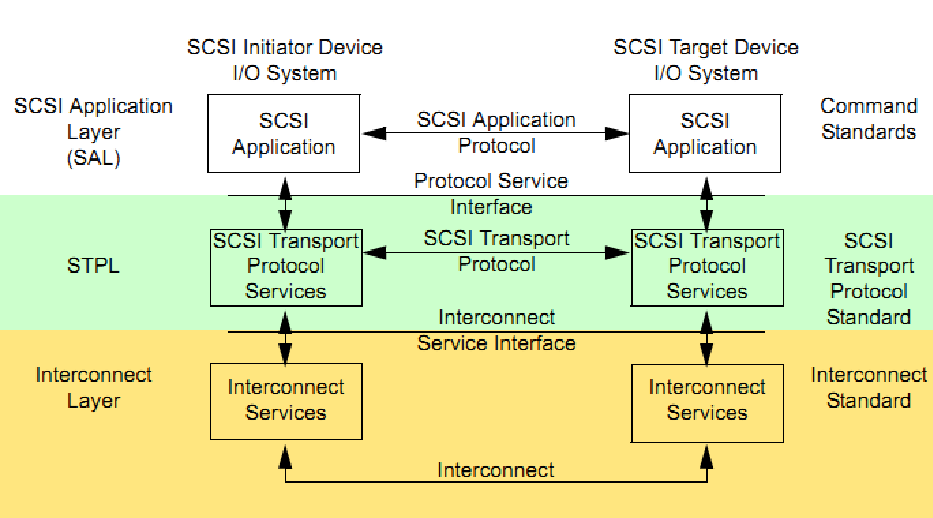
\includegraphics[width=14cm]{figs/scsiLayer.pdf}\\
  \caption{SCSI, modelo de camadas, adaptada de \cite{SCSI:Sam}}
  \label{FIG:ScsiLayer}
\end{figure}


Na Figura \ref{FIG:Scsi} a fam�lia de padr�es \ac{SCSI} � apresentada \cite{t10}. No topo da figura est�o o conjunto de comandos prim�rios\footnote{\emph{SCSI Primary Commands - 4 (SPC-4)}, vers�o mais recente.}, compartilhado por todos os tipos de dispositivos, e os conjuntos de comandos espec�ficos, utilizados por diferentes grupos de dispositivo, como os de comandos de blocos\footnote{\emph{SCSI Block Commands - 3 (SBC-3)}, vers�o mais recente.} (caso dos \acp{HD}), de \emph{stream}\footnote{\emph{SCSI Stream Commands - 4 (SSC-4)}, vers�o mais recente.}, de multim�dia\footnote{\emph{MultiMedia Command Set - 6 (MMC-6)}, vers�o mais recente.}, ou da controladora\footnote{\emph{SCSI Controller Commands-2 (SCC-2)}, vers�o mais recente.}, por exemplo.

No meio da figura est�o os protocolos de transporte, \ac{SAS}\footnote{\emph{SAS Protocol Layer - 3 (SPL-3)}}, \emph{fibre channel}\footnote{\emph{Fibre Channel Protocol - 4 (FCP-4)}, vers�o mais recente.}, \ac{iSCSI}, entre outros. Na base est�o as conex�es f�sicas, \ac{SAS}\footnote{\emph{Serial Attached SCSI - 3 (SAS-3)}, vers�o mais recente.}, \emph{fibre channel}, internet, \ac{USB}, \emph{PCI express}, entre outros. J� na lateral da figura est� o modelo de arquitetura \ac{SCSI}\footnote{\emph{SCSI Architecture Model - 5 (SAM-5)}, vers�o mais recente.}.
\begin{figure}[htb!]
  \centering
  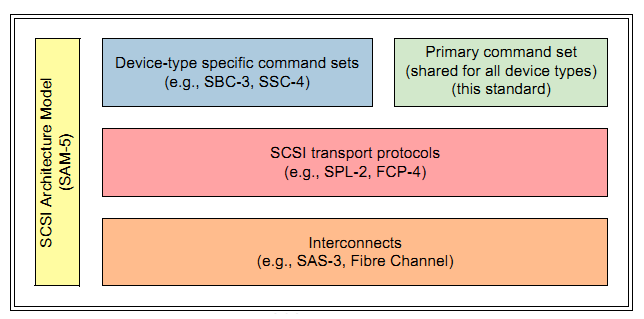
\includegraphics[width=14cm]{figs/scsi.png}\\
  \caption{Fam�lia de padr�es SCSI, adaptada de \cite{SCSI:Sam}}\label{FIG:Scsi}
\end{figure}

\subsection{ATA}

O padr�o \ac{ATA} foi desenvolvido para ser uma interface entre computadores e discos r�gidos. Inicialmente projetado para conectar placas-m�e e discos r�gidos com as novas vers�es passou a conectar dispositivos �pticos, como leitoras de \ac{CD}, \ac{DVD}, e \ac{BD}(\emph{BluRay Disc}), e tamb�m fitas magn�ticas, atrav�s do padr�o \ac{ATAPI}, que permite a transmiss�o de comandos \ac{SCSI} por conex�es \ac{ATA}.

O \ac{ATA} permite comunicar um \emph{host}, que pode ser um \emph{software}, o \ac{BIOS} ou um \emph{driver} de um sistema operacional,  a um dispositivo, que pode ser um disco r�gido ou um leitor �ptico, atrav�s de um subsistema de entrega. A Figura \ref{FIG:AtaLayer} mostra como essa comunica��o � realizada. O \emph{host} envia um comando, que passa por um protocolo de transporte, de onde � transmitido para o dispositivo atrav�s de uma conex�o f�sica. Ao chegar no dispositivo, o comando passa por um protocolo de transporte e � ent�o processado e executado por ele.

Assim como no padr�o \ac{SCSI}, os protocolos de transporte e interconex�es f�sicas n�o interferem no comando enviado. Logo, outros padr�es podem ser utilizados para transmitir comandos \ac{ATA}, como acontece com o padr�o \ac{SCSI}, que pode transmitir comandos \ac{ATA} atrav�s de uma camada de tradu��o\footnote{\emph{SCSI-ATA Translation}}. Comandos \ac{ATA} s�o encapsulados em comandos \textsc{ATA Pass-Through} e mandados atrav�s do \ac{SATA} ou \ac{PATA}, protocolos de transporte e de interconex�o f�sica \ac{SCSI}.

\begin{figure}[htb!]
  \centering
  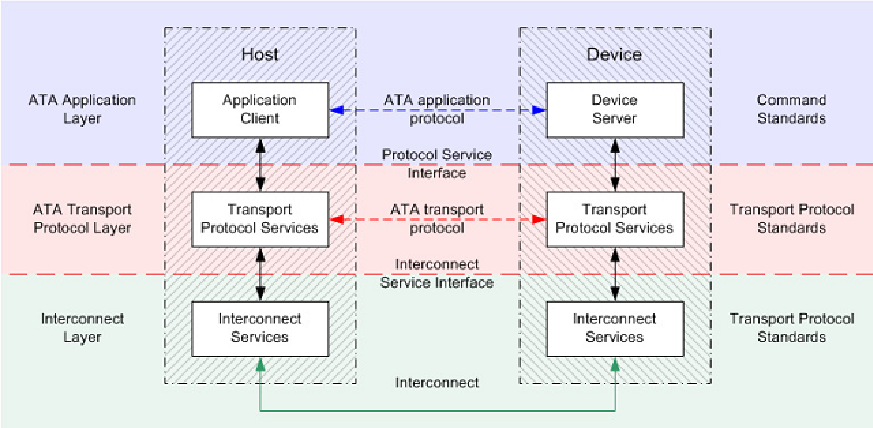
\includegraphics[width=14cm]{figs/ataLayer.pdf}\\
  \caption{ATA, modelo de camadas, adaptada de \cite{ATA8:AAM}}\label{FIG:AtaLayer}
\end{figure}

O desenvolvimento do \ac{ATA} � guiado por um modelo abstrato, especificado atrav�s de diversos documentos, tamb�m chamados de padr�es, como descrito na Figura \ref{FIG:Ata}, adaptada de \cite{ATA8:AAM}. Nela tem-se o modelo de arquitetura\footnote{\emph{ATA/ATAPI Architecture Model (ATA8-AAM)}, vers�o mais recente.}, que define o modelo de sistema e especifica��es, o conjunto de comandos\footnote{\emph{ATA/ATAPI Command Set (ATA8-ACS)}, vers�o mais recente.}, o conjunto de comandos de entrega, que s�o documentos \ac{SCSI} e \ac{ATAPI}, e os padr�es de transporte  \ac{PATA} e \ac{SATA}.


\begin{figure}[htb!]
  \centering
  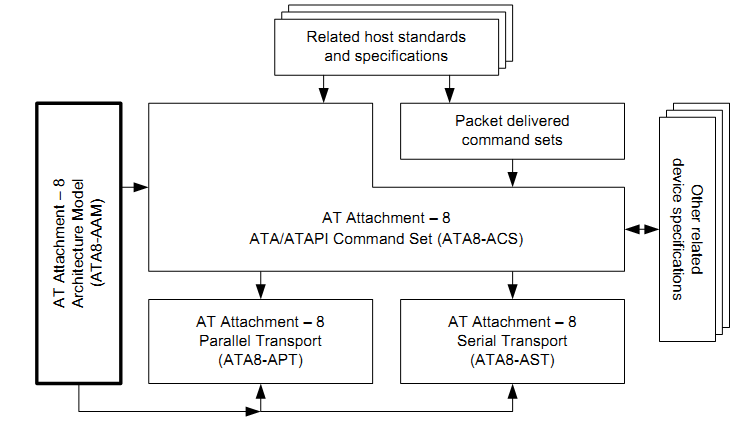
\includegraphics[width=14cm]{figs/ata.png}\\
  \caption{Fam�lia de padr�es ATA}\label{FIG:Ata}
\end{figure}

\newpage
\section{Resumo do Cap�tulo}

Neste capitulo foram explorados os conceitos de falha, erro e defeito, o diagn�stico de falhas, bem como os tipos de falha que ocorrem em discos r�gidos. O sistema \ac{SMART} e os protocolos \ac{ATA} e \ac{SCSI}, que s�o a base de desenvolvimento deste trabalho, foram apresentados.

No pr�ximo cap�tulo a metodologia utilizada neste trabalho e o desenvolvimento deste trabalho s�o apresentados.

%Neste cap\'{\i}tulo foram descritos as ferramentas utilizadas no desenvolvimento deste trabalho, os gestos que podem ser reconhecidos pelo sistema e tr\^{e}s m\'{e}todos de se extrair atributos para treinamento propostos neste trabalho. Tamb\'{e}m foi descrito neste cap\'{\i}tulo os passos para realizar o treinamento e classifica\c{c}\~{a}o dos gestos, e quais os m\'{e}todos de compara\c{c}\~{a}o utilizado para se avaliar cada m\'{e}todo. No cap\'{\i}tulo seguinte, s\~{a}o apresentados os resultados dos testes de simula\c{c}\~{a}o para cada um dos m\'{e}todos.


%\begin{tabular}{|l|l|l|} \hline
%\multicolumn{3}{|c|}{Schedulers} \\ \hline
% RR & \multirow{3}{*}{Immediate}  & Round Robin \\ \cline{1-1} \cline{3-3}
% EF   & & Earliest First  \\ \cline{1-1} \cline{3-3}
% LL  & &  Lightest Loaded  \\ \hline
%\multirow{4}{*}{Batch} & MM & Min-Min \\
%& MX & Max-Min \\
%& DL & Dynamic Level \\
%& RC & Relative Cost \\ \hline
%\multirow{4}{*}{Evolutionary} & PN & This paper \\
%& ZO & Genetic Algorithm\\
%& TA & Tabu search~\cite{GLOV1986j}\\
%& SA & Simlulated Annealing \\ \hline
%\end{tabular}

%%%%%%%%%%%%%%%%%%%%%%%%%%%%%%%%%%%%%%%%%%%%%%%%%%%%%%%%%%%%%%%%%
%%%% CAP�TULO 4: Metodologia e Implementa��o
\chapter{Metodologia e Implementa��o} \label{CHP:MET}%%

Este cap�tulo apresenta as metodologias de desenvolvimento e de teste utilizadas neste projeto, bem como os detalhes de implementa��o do \emph{framework} proposto e os algoritmos implementados.  Na Se��o \ref{implementacao} as estrat�gias de implementa��o dos comandos \ac{ATA} e \ac{SCSI} s�o apresentadas, as abordagens adotadas s�o discutidas e � feito o detalhamento do \emph{framework}, da camada de aplica��o e do \emph{Bootable} criado.

A Se��o \ref{metodologia} descreve o ambiente de desenvolvimento e os recursos utilizados, comenta o m�todo de inser��o de falhas utilizado e descreve a metodologia de teste.

\section{Metodologia}\label{metodologia}
 
No desenvolvimento deste trabalho, foram utilizados diversos \acp{HD}, para valida��o dos comandos e algoritmos, \emph{laptops} e \emph{desktops}, para realiza��o dos teste e valida��o do funcionamento do \emph{Bootable}. Todos os computadores e \acp{HD} utilizados, exceto o computador pessoal da autora, fazem parte do acervo do \ac{LESC}\footnote{Laborat�rio de pesquisa e desenvolvimento com vasta experi�ncia no desenvolvimento de \emph{softwares} de diagn�stico para linhas de produ��o e usu�rios finais.}, da \ac{UFC}.

Na valida��o dos comandos foram gerados pequenos m�dulos execut�veis para que os comandos pudessem ser validados individualmente. Foi desenvolvido um m�todo de inser��o de falha descrito na Se��o \ref{insercaofalha}, usado para validar os comandos e os algoritmos de teste.

\subsection{Inser��o de Falhas}\label{insercaofalha}
Na valida��o dos algoritmos foram utilizados \acp{HD} em boas condi��es, sem falhas detectadas por outras ferramentas de diagn�stico, nos quais foram ``inseridos'' falhas em alguns setores, atrav�s do comando \ac{ATA} \textsc{Write Uncorrectable (45h)}. Com este comando � poss�vel configurar setores para que retornem \emph{status} de falha, quando um comando de leitura for executado. H� duas op��es dispon�veis, criar um erro pseudo incorrig�vel, com \emph{log}, e criar um erro sinalizado, sem \emph{log}. Na primeira op��o, quando um comando de leitura for executado, o erro de leitura ser� inclu�do nos \emph{logs} da controladora e do \ac{SMART} e na segunda op��o o comando retornar� erro, mas este n�o ser� inserido nos \emph{logs}. Neste trabalho utilizou-se a primeira op��o, para ajudar na valida��o de comandos, como \textsc{Read Log Ext (2Fh)}, e na implementa��o de testes, como o \emph{Targeted Read}, que se baseia na leitura dos \emph{logs} armazenados.

Para remover a falha inserida � necess�rio realizar um comando de escrita no setor configurado, o dado armazenado ser� perdido e o setor n�o retornar� \emph{status} de erro na realiza��o de novos comandos de leitura, a menos, � claro, que este setor se torne realmente falho. Neste trabalho utilizou-se os comandos \textsc{Write Sector(s) (30h)} e \textsc{Write Sector(s) Ext (34h)} para remover as falhas ``inseridas''.

\subsection{Metodologia de Teste}\label{metodologiateste}

Os testes foram realizados utilizando discos r�gidos com falhas conhecidas,  detectadas por outros \emph{softwares}, no caso Lenovo \emph{ThinkVantage ToolBox}, desenvolvido pela PC-Doctor dispon�vel nos computadores Lenovo e executado no Windows, e \emph{smartmootools}, executado no Linux.

Os algoritmos implementados foram testados utilizando 12 \acp{HD} nos quais estes algoritmos foram executados. Destes \acp{HD} 9 s�o do tipo \ac{HDD} e 3 do tipo \ac{SSD}, entre eles h� \acp{HD} com falhas e \acp{HD} em perfeito estado de funcionamento. Foram utilizados discos de dois tipos de \emph{form factor}, $2.5 in$ e $3.5 in$.  Uma sequ�ncia de algoritmos foi definida e executada 3 vezes para cada dispositivo. Os resultados foram comparados e est�o descritos no Cap�tulo \ref{CHP:RESULT}.

\section{Implementa��o} \label{implementacao}

O intuito deste trabalho � o desenvolvimento de um \emph{framework} para dar suporte ao desenvolvimento de testes  de diagn�stico para serem executados em \emph{desktops} e \emph{laptops}.  Neste trabalho alguns testes foram implementados, apenas para demonstrar a efici�ncia do \emph{framework} e servir de base para uma an�lise preliminar sobre a validade dos mesmos, pois, tendo em vista que para uma an�lise estat�stica confi�vel destes algoritmos seria necess�ria uma grande quantidade de discos r�gidos, varia��es de par�metros e repeti��es de testes, e n�o seria poss�vel concluir no tempo previsto, de um semestre.

Como dito anteriormente, a capacidade de armazenamento dos discos r�gidos vem crescendo fortemente. Testar todos os setores de um disco r�gido pode levar muitas horas e \emph{softwares} de diagn�stico como PC-Doctor, Aida32 e Hard Disk Sentinel, oferecem testes r�pidos, que analisam amostras de setores, que levam de 5 a 10 minutos, e � para o desenvolvimento deste tipo de teste que o \emph{framework} foi pensado.

Na Se��o \ref{eolinux} a implementa��o dos comandos \ac{ATA} e \ac{SCSI} no Linux � descrita. O \emph{framework} proposto � descrito na Se��o \ref{framework} e o \emph{bootable} na Se��o \ref{bootable}.


\subsection{ATA, SCSI, SMART e o Linux} \label{eolinux}

No Linux, lidar com dispositivos \ac{SCSI} e \ac{ATA} � bastante simples, similar ao trato de arquivos de entrada e sa�da padr�o. Os comandos s�o enviados aos dispositivos atrav�s dos \emph{drivers}, \emph{softwares} que conectam o sistema operacional ao \emph{hardware} do computador \cite{Tanenbaum:2001}.

Os dispositivos correspondem a arquivos no diret�rio \emph{/dev}  e utilizam-se de chamadas de sistema, por exemplo, para comand�-los. Usa-se a chamada \emph{open()} para criar um descritor para o dispositivo, como mostrado no pr�ximo par�grafo. Uma vez criado o descritor, os comandos podem ser escritos e lidos atrav�s dele com as chamadas \emph{read()}, \emph{write()} ou \emph{ioctl()}, como descrito em \cite{Final}, \cite{SCSI:programming}.

\begin{quote}
\textsf{int fd = open (device\_name, O\_RDWR);}
\end{quote}

Discos \ac{SCSI} s�o acessados atrav�s do \emph{driver} \emph{sd}, para discos r�gidos,  e \emph{sg}, para quaisquer dispositivos \ac{SCSI}, ambos disponibilizados pelo pacote sg3-utils. Neste trabalho, os dados ser�o escritos e lidos usando a estrutura sg\_io\_hdr\_t, descrita em (\emph{scsi/sg.h}) e a seguir, enviadas atrav�s do \emph{driver sg}.


\begin{quote}
\textsf{int dxfer\_direction: especifica a dire��o da transfer�ncia de dados.\\unsigned char *dxferp: ponteiro para os dados transferidos.\\unsigned char * cmdp: ponteiro para o comando.\\ unsigned char * sbp: ponteiro para o sense buffer.\\  unsigned char masked\_status: status GOOD ou CHECK CONDITION.}
\end{quote}

Os comandos \ac{SCSI} t�m,  em geral, 6, 10, 12 ou 16 \emph{bytes} de tamanho e s�o enviados no formato de um bloco descritor de comando, que � um dos campos da estrutura sg\_io\_hdr\_t e cont�m \emph{opcode} do comando, \ac{LBA} (endere�o do setor), tamanho em \emph{bytes} a ser transferido e outras flags de comando, como descrito na Figura \ref{FIG:scsi10}, um comando de 10 bytes.

Depois de receber um comando, o dispositivo \emph{alvo} responde com um \emph{byte} de \emph{status} e retorna uma estrutura chamada sense buffer com mais informa��es. Utilizam-se algumas abordagens mostradas em \cite{Final}, \cite{Tao:2009}, quanto ao uso das chamadas \emph{read()/write()} ou \emph{ioctl}. Neste trabalho foi adotado o uso da chamada \emph{ioctl}, que equivale ao uso de uma chamada \emph{write()} seguida de uma chamada \emph{read()}. No caso de um comando que retorne erro, usando \emph{read()/write()}, � necess�rio o envio de outro comando, o \textsc{Request Sense}, para obter mais informa��es sobre o problema; com o uso do \emph{ioctl()} a pr�pria estrutura j� retorna todas as informa��es, no campo \emph{sense\_buffer}. No pr�ximo par�grafo o envio de um comando por \emph{ioctl()} � descrito, onde fd � o descritor do dispositivo, p\_hdr � uma instancia��o da estrutura sg\_io\_hdr\_t e SG\_IO � o par�metro referente ao \emph{driver sg}.

\begin{quote}
\textsf{int ret = ioctl(fd, SG\_IO, p\_hdr);}
\end{quote}

%\begin{table}[htb!]
   % \begin{center}
\begin{figure}%[htb!]
  \centering
  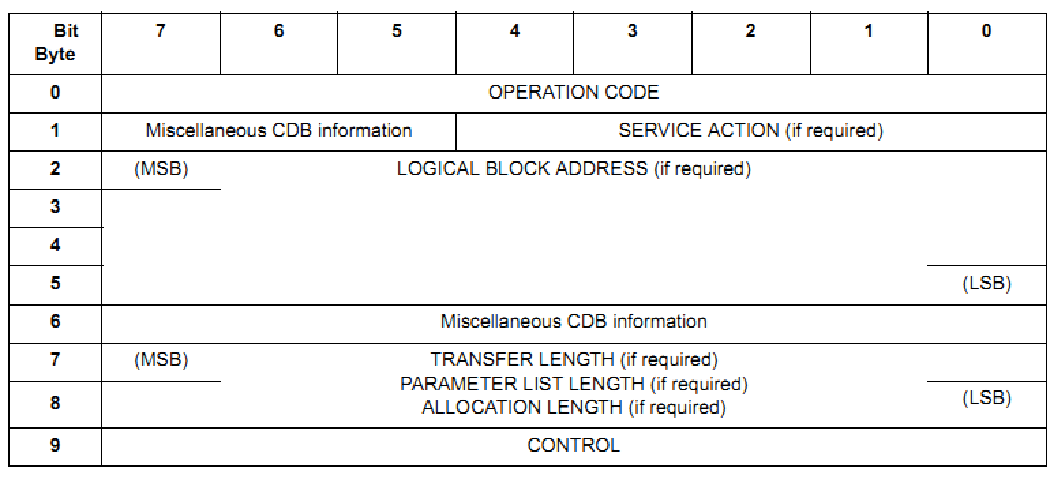
\includegraphics[width=14cm]{figs/scsiCdb.pdf}\\
  %\caption{Fam�lia de padr�es ATA}\label{FIG:Ata}
    \caption{Comando de 10 bytes t�pico, adaptado de \cite{SCSI:Sam}}
    \label{FIG:scsi10}
\end{figure}

O processamento em  discos \ac{SATA}/\ac{ATA} � um pouco diferente, pois algumas vezes, as controladoras \ac{SATA} est�o conectadas atrav�s de um barramento do tipo PCI, o que leva o sistema operacional a interpret�-lo como um adaptador de barramento\footnote{\emph{Host Bus Adapter (HBA).}} \ac{SCSI} \cite{SCSI:toolbox}. Isto impossibilita o envio de comandos \ac{ATA} aos discos, para ter acesso aos discos utiliza-se a camada de tradu��o \ac{SCSI}-\ac{ATA}, que encapsula comandos \ac{ATA} em comandos \ac{SCSI}, provida no Linux pela biblioteca libATA \cite{Bart:2010}, fazendo uso do comando \textsc{ATA Pass-Through}. A camada de tradu��o � descrita em \cite{SCSI:ATAtranslation} e o comando � detalhado em \cite{SCSI:AtaPassThrough}. Como o sistema \ac{SMART} � especificado pelo padr�o \ac{ATA}, os comandos de \ac{SMART} tamb�m s�o enviados via \textsc{ATA Pass-Through}.

O envio de comandos via \textsc{ATA Pass-Through} apresentou alguns detalhes peculiares durante o desenvolvimento. A ordem de preenchimento da estrutura de dados do comando a ser enviado influencia no resultado do comando. Na Figura \ref{FIG:atapassthrough} a estrutura do comando � apresentada. Diversos testes foram realizados em diferentes discos r�gidos e verificou-se que apenas quando os campos \emph{LBA\_LOW(0:7)},  \emph{LBA\_MID(0:7)},  \emph{LBA\_HIGH(0:7)} eram preenchidos em sequ�ncia o comando respondia adequadamente. N�o foram encontradas refer�ncias a isso na documenta��o dos padr�es \ac{ATA} e \ac{SCSI}, apenas uma sequ�ncia de bytes comentados em um c�digo fonte que implementava um dos comandos \ac{SCSI}. Outro detalhe � que a resposta dos comandos enviados via \textsc{ATA Pass-Through} varia de acordo com o fabricante, pois uma certa quantidade de \emph{bytes} � coletada antes da estrutura que descreve a resposta. Esta quantidade varia de acordo com o fabricante, em torno de 22 \emph{bytes}, depois destes \emph{bytes} a sequ�ncia de \emph{bytes} 09h 0ch marca o in�cio da estrutura de descri��o de resultados, tamb�m n�o h� refer�ncia a isto nas documenta��es dos padr�es \ac{ATA} e \ac{SCSI}.

\begin{figure}%[htb!]
  \centering
  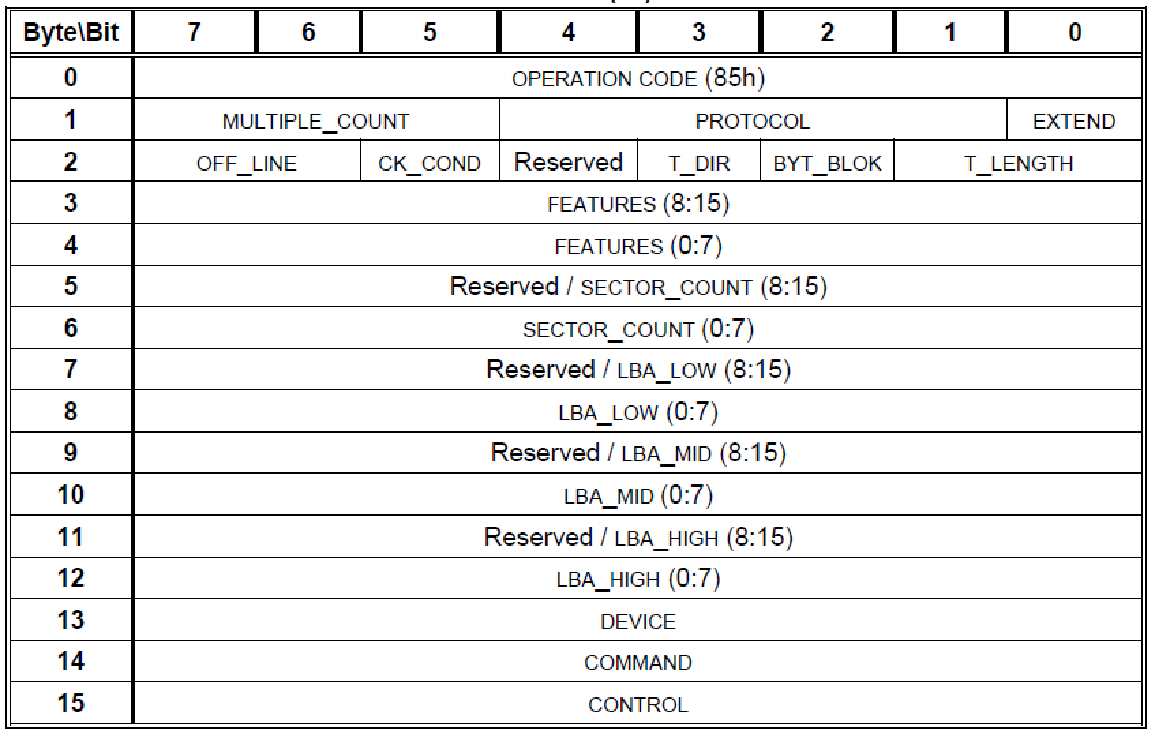
\includegraphics[width=14cm]{figs/atapassthrough.pdf}\\
  %\caption{Fam�lia de padr�es ATA}\label{FIG:Ata}
    \caption{Comando ATA Pass-Through, adaptado de \cite{SCSI:AtaPassThrough}}
    \label{FIG:atapassthrough}
\end{figure}


\subsection{\emph{Framework} Proposto} \label{framework}

O \emph{framework} foi implementado em linguagem C++, escolhida por reunir caracter�sticas de linguagens de alto e baixo n�vel. Esta foi desenvolvida para ser compat�vel e t�o eficiente e port�vel quanto a linguagem C e suporta m�ltiplos paradigmas de programa��o, principalmente a programa��o estruturada e a programa��o orientada a objetos.

Os padr�es \ac{ATA} e \ac{SCSI} disponibilizam v�rios tipos de comandos, desde comandos simples para a leitura de informa��es sobre o fabricante do dispositivo at� comandos para aplica��es de seguran�a, e nem todos os comandos s�o �teis para este trabalho, que se prop�e a execu��o de algoritmos de leitura e testes \ac{SMART}. Alguns comandos foram selecionados e s�o listados nesta Se��o. Foram implementados os principais comandos de leitura e verifica��o de \acp{LBA}, comandos \ac{SMART} e de auto-teste e comandos para leitura dos \emph{logs} gerados pela controladora. Estes \emph{logs} cont�m informa��es como os comandos que retornaram erro e em que \acp{LBA} eles foram executados, como descrito na Se��o \ref{falhashd}, isto � um recurso �til para a verifica��o de falhas tempor�rias e checagem da vizinhan�a.

O \emph{framework} � descrito como um diagrama de classes na Figura \ref{FIG:Framework}. Nesta Figura, a classe \emph{ScsiCmd} implementa a estrutura de um comando \ac{SCSI}, bem como as suas funcionalidades, v�rias classes s�o herdeiras da classe \emph{ScsiCmd}, entre elas a classe \emph{ATAPassThrough}, de onde os comandos \ac{ATA}, entre eles o \ac{SMART}, herdam suas caracter�sticas.

Neste diagrama s�o descritas apenas as classes que implementam comandos \ac{ATA} e \ac{SCSI} e que foram utilizadas na implementa��o de testes. Todos os comandos implementados s�o detalhados nas Tabelas \ref{TAB:scsi_selected} e \ref{TAB:ata_selected}. As classes \emph{Inquiry}, \emph{ModeSense}, \emph{ReadCapacity}, \emph{Read}, \emph{Verify} e \emph{TestUnitRead} implementam comandos \ac{SCSI} puros e podem ser usados para outros tipos de dispositivos. No centro do diagrama est� a classe \emph{AtaPassThrough}, dela s�o herdeiras as classes \emph{ReadVerify}, \emph{ReadVerifyExt}\footnote{A diferen�a entre \emph{ReadVerify} e \emph{ReadVerifyExt}, assim como \emph{ReadSector} e \emph{ReadSectorExt}, � o tamanho da ac{LBA} endere�ada. Os comandos ``Ext'' utilizam \ac{LBA} de 48 bits e os outros de 28 bits.}, \emph{ReadSector}, \emph{ReadSectorExt}, \emph{Identify}, \emph{ReadLogExt}, \emph{WriteSector}, \emph{WriteUncorrectable} e \emph{SmartCmd}, estes comandos s�o \ac{ATA}. As classes ligadas � \emph{SmartCmd} implementam um mesmo comando, que cont�m v�rias funcionalidades diferentes. S�o elas: \emph{SmartStatus}, \emph{EnableSmart}, \emph{DisableSmart}, \emph{SmartReadLog}, \emph{AbortSelfTest}, \emph{ShortSelfTestSmart}, \emph{ExtendedSelfTestSmart} e \emph{ConveyanceSelfTestSmart}.

\begin{figure}[htb!]
  \centering
  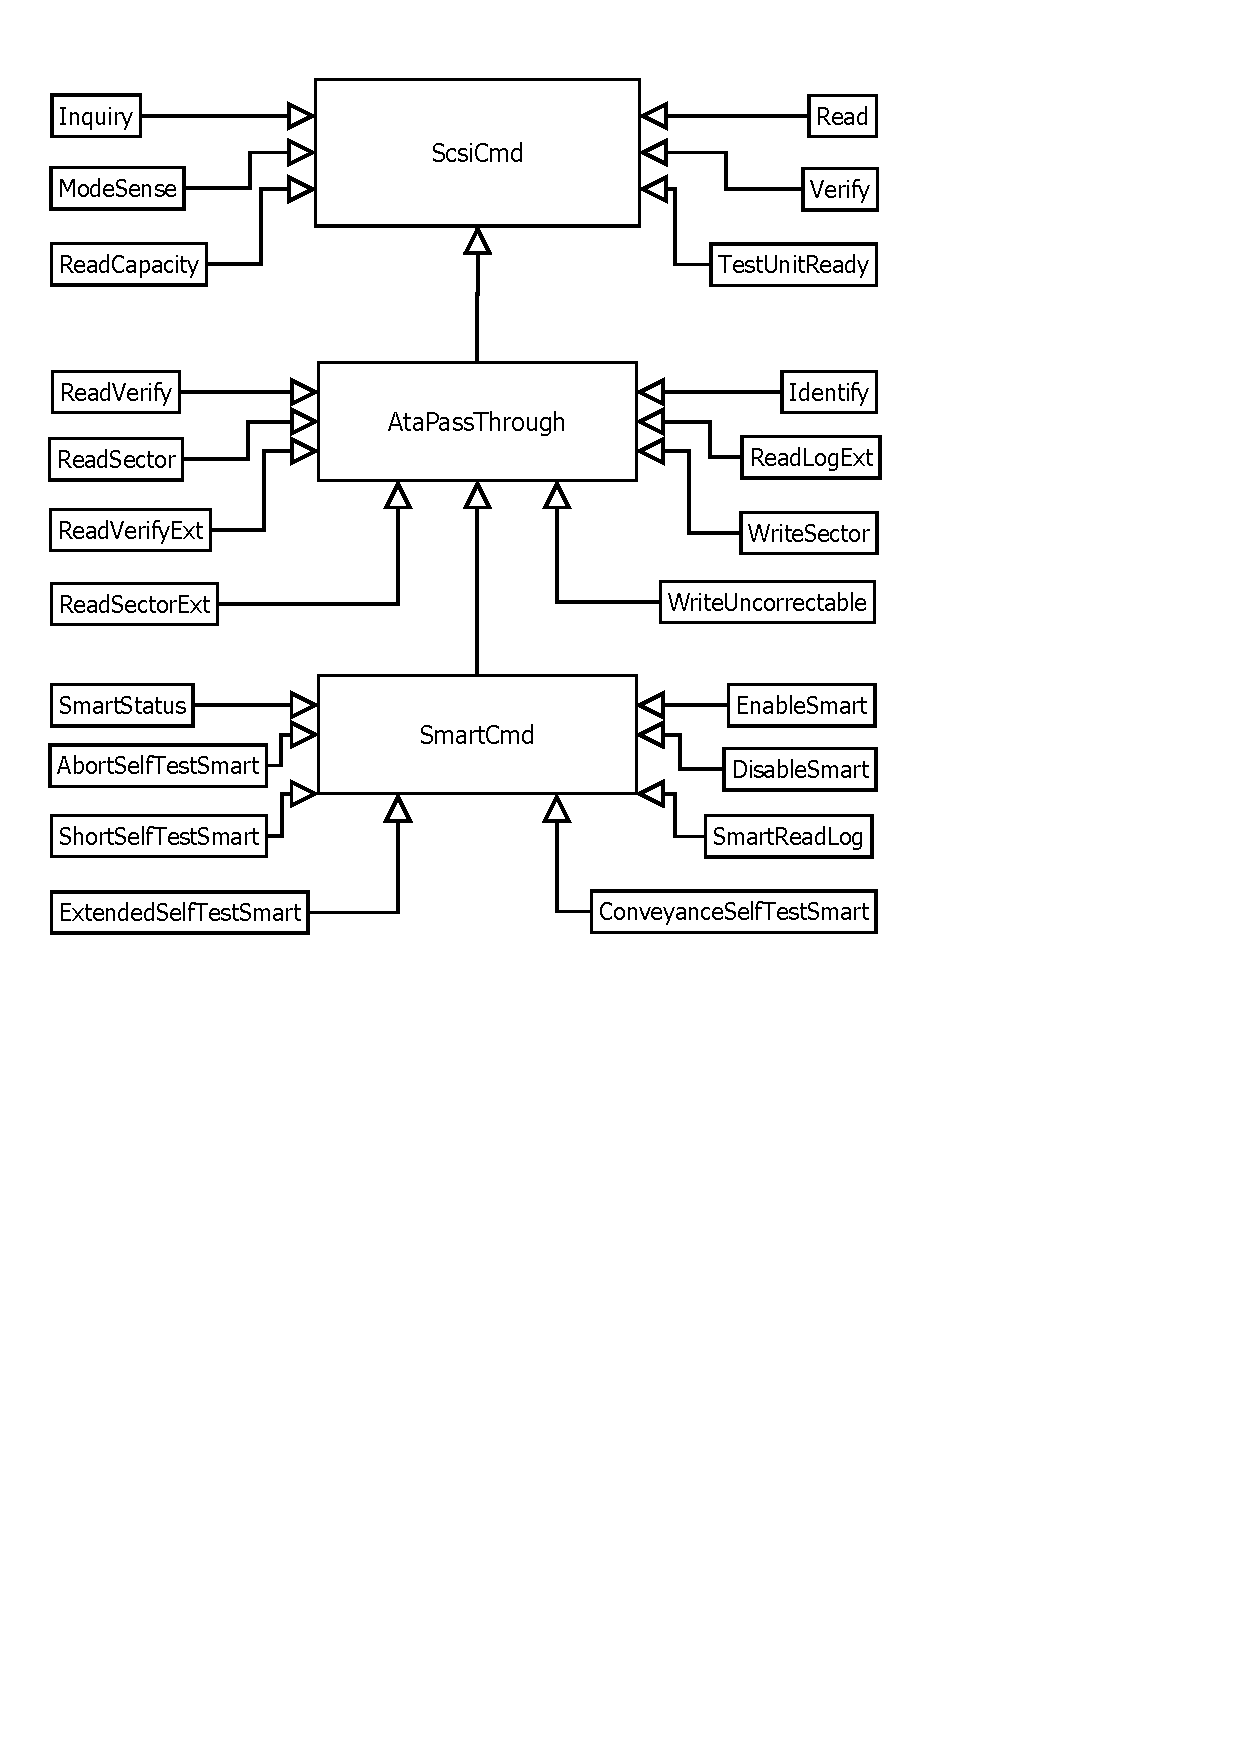
\includegraphics[width=14cm]{figs/framework.pdf}\\
  \caption{Diagrama de Classes do Framework}\label{FIG:Framework}
\end{figure}

A Tabela \ref{TAB:scsi_selected}, descreve  os comandos \ac{SCSI} implementados e a Tabela \ref{TAB:ata_selected} os comandos \ac{ATA}, enviados via \textsc{ATA Pass-Through}.


\begin{table}
    \caption{Comandos \ac{SCSI} selecionados em ordem alfab�tica}
    \label{TAB:scsi_selected}
    \vspace{-10pt}
    \begin{center}
       \begin{tabular}{|p{5 cm}|c|p{7 cm}|}
         \hline
         % after \\: \hline or \cline{col1-col2} \cline{col3-col4} ...
         Comando & C�digo  & Descri��o  \\ \hline
         \textsc{ATA Pass-Through (16)} & 85h & Este comando permite o envio encapsulado de comandos \ac{ATA} atrav�s de comandos \ac{SCSI}  \\ \hline
         \textsc{Inquiry} & 12h & Permite coletar informa��es sobre o dispositivo, o fabricante entre outros.  \\   \hline
         \textsc{Log Select} & 4Ch &  Permite coletar informa��es dos \emph{logs} da controladora. \\ \hline
         \textsc{Log Sense} & 4Dh & Permite coletar informa��es dos \emph{logs} da controladora. Funciona em conjunto com o comando \textsc{Log Select}   \\ \hline
         \textsc{Mode Sense (6)} & 1Ah &   Permite coletar informa��es de p�ginas espec�ficas do dispositivo. \\    \hline
         \textsc{Read (10)} & 28h &   Permite a leitura de um setor espec�fico do dispositivo. Requisita a transfer�ncia de dados. \\   \hline
         \textsc{Read Capacity (10)} & 25h &   Permite coletar informa��es sobre a capacidade do dispositivo, devolve a �ltima \ac{LBA} v�lida.  \\    \hline
         \textsc{Read Defect Data (10)} & 37h &  Permite coletar informa��es sobre os setores defeituosos no dispositivo.* \footnote{*Comando voltado para o desenvolvimento de testes em discos \ac{SCSI}, ainda n�o validados por n�o haver dispositivos compat�veis no Laborat�rio. }  \\ \hline 
         \textsc{Reassign Blocks} & 07h &   Envia a requisi��o para que a controladora remapei os setores defeituosos.*  \\   \hline
         \textsc{Receive Diagnostic Results} & 1Ch   & Permite coletar informa��es da p�gina espec�fica de diagn�stico. Usado em conjunto com \textsc{Send Diagnostic}.  \\    \hline
         \textsc{Send Diagnostic} & 1Dh &   Requisita a execu��o de auto-testes pelo dispositivo. \\   \hline
         \textsc{Test Unit Ready} & 00h &  Testa se a unidade est� pronta para receber comandos   \\ \hline
         \textsc{Verify (10)} & 2Fh  &   Realiza a verifica��o de um setor, compara o conte�do do setor e os c�digos de checagem de erro. \\   \hline
          \end{tabular}
    \end{center}
    \vspace{-15pt}
\end{table}

\begin{table}
    \caption{Comandos \ac{ATA} selecionados em ordem alfab�tica}
    \label{TAB:ata_selected}
    \vspace{-10pt}
    \begin{center}
       \begin{tabular}{|p{5 cm}|c|p{8 cm}|}
         \hline
         % after \\: \hline or \cline{col1-col2} \cline{col3-col4} ...
         Comando & C�digo  & Descri��o  \\ \hline
         \textsc{Read Sector} & 20h  & Usado para ler o conte�do de um ou mais setores \\ \hline
         \textsc{Read Sector Ext} & 24h  & Usado para ler o conte�do de um ou mais setores \\ \hline
         \textsc{Read Verify Sectors} & 40h  & Usado para verificar o conte�do de um ou mais setores \\ \hline
         \textsc{Read Verify Sectors Ext} & 44h  & Usado para verificar o conte�do de um ou mais setores \\ \hline
         \textsc{SMART} & B0h & Este comando implementa diferentes funcionalidades relacionadas com o sistema \ac{SMART}, que foram implementadas em diferentes classes no \emph{framework} proposto. S�o eles:
         \begin{itemize}
                                                \item \textsc{Diasable Operations (B0h/D9h)}
                                                \item \textsc{Enable Operations (B0h/D8h)}
                                                \item \textsc{Execute off-line immediate (B0h/D4h)}, este subcomando executa os auto-testes \ac{SMART}, que s�o determinados atrav�s dos par�metros passados na estrutura do comando.
                                                \item \textsc{Read Data (B0h/D0h)}
                                                \item \textsc{Read Log (B0h/D5h)}
                                                \item \textsc{Return Status (B0h/DAh)}
                                              \end{itemize} \\ \hline
         \textsc{Write Sector} & 30h & Usado para escrever dados em um ou mais setores \\ \hline
         \textsc{Write Uncorrectable} & 45h  & Usado para inserir erros \\ \hline


       \end{tabular}
    \end{center}
    \vspace{-15pt}
\end{table}

\subsection{Camada da Aplica��o}

Na camada de aplica��o os algoritmos de teste s�o implementados e tamb�m outras fun��es para auxiliar na execu��o do teste como fun��es de listagem de dispositivos, filtragem de \emph{pendrives} e discos r�gidos externos, tratamento de \emph{strings} e uso de express�o regular, que n�o ser�o detalhados aqui por n�o ser o foco deste trabalho.

Os testes s�o voltados para computadores em uso. Logo, eles n�o podem realizar escritas no disco r�gido, pois isso poderia corromper os dados ou o sistema de arquivos do usu�rio. Os dispositivos \acp{SSD} tem comportamento f�sico ``similar'' a mem�rias \ac{RAM}, para as quais existem v�rios testes consagrados como os testes do tipo \emph{MARCH}, \emph{Moving Inversion}, \emph{GALPAK} \cite{adams2003high}. Entretanto, todos estes algoritmos utilizam opera��es de escritas na verifica��o da mem�ria, o que impossibilita o seu uso para diagn�stico de discos r�gidos.

Os algoritmos implementados s�o de dois tipos,  \ac{SMART} e de busca, que se baseiam na descri��o dada nos manuais de ajuda pelos \emph{softwares} de diagn�stico, pois como se trata de uma linha de estudo bastante comercial, h� pouca ou nenhuma informa��o sobre eles. Os algoritmos s�o descritos a seguir:
% Explicar porque Read Verify em vez de Read.

\begin{itemize}
  \item \ac{SMART} \emph{Return Status} executa o comando \ac{SMART} \emph{Return Status} e verifica se as medidas coletadas excedem o limiar m�ximo. Este comando retorna um alerta bin�rio do tipo: Ir� Falhar/N�o Ir� Falhar. Este alerta pretende avisar ao usu�rio quanto � probabilidade de o sistema falhar durante as pr�ximas 24 horas de funcionamento.
  \item \ac{SMART} \emph{Short Self-Test} executa o comando \ac{SMART} \emph{Execute off-line immediate}, com o subcomando \emph{Execute SMART short self-test routine in off-line mode}.
  \item \ac{SMART} \emph{Extended Self-Test} executa o comando \ac{SMART} \emph{Execute off-line immediate}, com o subcomando \emph{Execute SMART extended self-test routine in off-line mode}.
  \item \ac{SMART} \emph{Conveyance Self-Test}  executa o comando \ac{SMART} \emph{Execute off-line immediate}, com o subcomando \emph{Execute SMART conveyance self-test routine in off-line mode}.
  \item \emph{Linear Seek} executa leituras com o comando \textsc{Read Verify} de modo que as leituras sejam feitas com o mesmo espa�amento, como descrito na Figura 4.4.a. O espa�amento utilizado � calculado em fun��o do tamanho do disco e  5000 setores s�o analisados. Se algum setor falho for encontrado o teste ser� encerrado.
      \begin{itemize}
        \item \emph{Linear Seek 1} Inicia o teste da menor para a maior \ac{LBA}.
        \item \emph{Linear Seek 2} Inicia o teste da maior para a menor \ac{LBA}.
      \end{itemize}
  \item \emph{Funnel Seek} executa leituras com o comando \textsc{Read Verify}, de modo que as leituras sejam feitas em dois sentidos, o algoritmo alternar� leituras da menor \ac{LBA} para a maior e da maior para a menor \ac{LBA} , como descrito na Figura 4.4.b. Se algum setor falho for encontrado o teste ser� encerrado.
      \begin{itemize}
        \item \emph{Funnel Seek 1} Neste algoritmo s�o utilizados dois passos, um passo fixo de 350.000 \acp{LBA} e um passo aleat�rio limitado a 10.000 \acp{LBA}. Uma vari�vel � utilizada para monitorar a condi��o de parada. A cada execu��o um n�mero de LBA � gerado somando a posi��o atual, iniciada em zero, o passo fixo e o passo aleat�rio. Esta LBA � analisada, primeiro sentido, e tamb�m a LBA correspondente ao valor total de LBAs menos o n�mero gerado, segundo sentido. O teste termina quando a LBA gerada no primeiro sentido for maior ou igual ao valor total de LBAs.
      \item \emph{Funnel Seek 2} Realiza o mesmo procedimento do \emph{Funnel Seek 1}, entretanto no in�cio do teste as 100 primeiras LBAs s�o analisadas e no final do teste a primeira e a �ltima LBAs s�o analisadas.
      \end{itemize}
  \item \emph{Random Seek} executa leituras com o comando \textsc{Read Verify} de modo que um percentual do disco seja analisado e as leituras sejam feitas de maneira aleat�ria, como descrito na Figura 4.5.a. Se algum setor falho for encontrado o teste ser� encerrado.
   \begin{itemize}
     \item \emph{Random Seek 1} executa leituras em 5000 setores.
     \item \emph{Random Seek 2} executa leituras em 7500 setores.
     \item \emph{Random Seek 3} executa leituras em 10000 setores.
   \end{itemize}
  \item \emph{Surface Scan} executa leituras com o comando \textsc{Read Verify}. As leituras s�o  feitas com o mesmo espa�amento para cada passo dado. Um grupo de setores ou trecho da superf�cie � analisado, como descrito na Figura 4.5.b.  Se algum setor falho for encontrado o teste ser� encerrado.
    \begin{itemize}
      \item \emph{Surface Scan 1} Divide o Disco em 2.000 ``lotes'' de setores e para cada in�cio de ``lote'' 30 setores s�o analisados. O algoritmo come�a executando da menor para a maior LBA.
      \item \emph{Surface Scan 2} Mesmo procedimento do \emph{Surface Scan 1}, mas segue o sentido oposto, come�a executando da maior para a menor LBA.
    \end{itemize}
  \item \emph{Targeted Read Test} este teste realiza a leitura do \emph{log} de falhas da controladora, identifica os setores listados e realiza novas leituras, nos setores e na sua vizinhan�a, para determinar se o mesmo continua com falhas. Cada LBA encontrado nos \emph{logs} � analisada e tamb�m os 5 setores anteriores e posteriores a ele. Este teste � comentado em \cite{PCdoc} e descrito na Figura 4.6. O teste � finalizado quando todos os setores listados ou quando mais de 5 setores falhos s�o encontrados.

\end{itemize}

\begin{figure}[htb!]
    \centering
    \subfigure[a][Linear Seek]{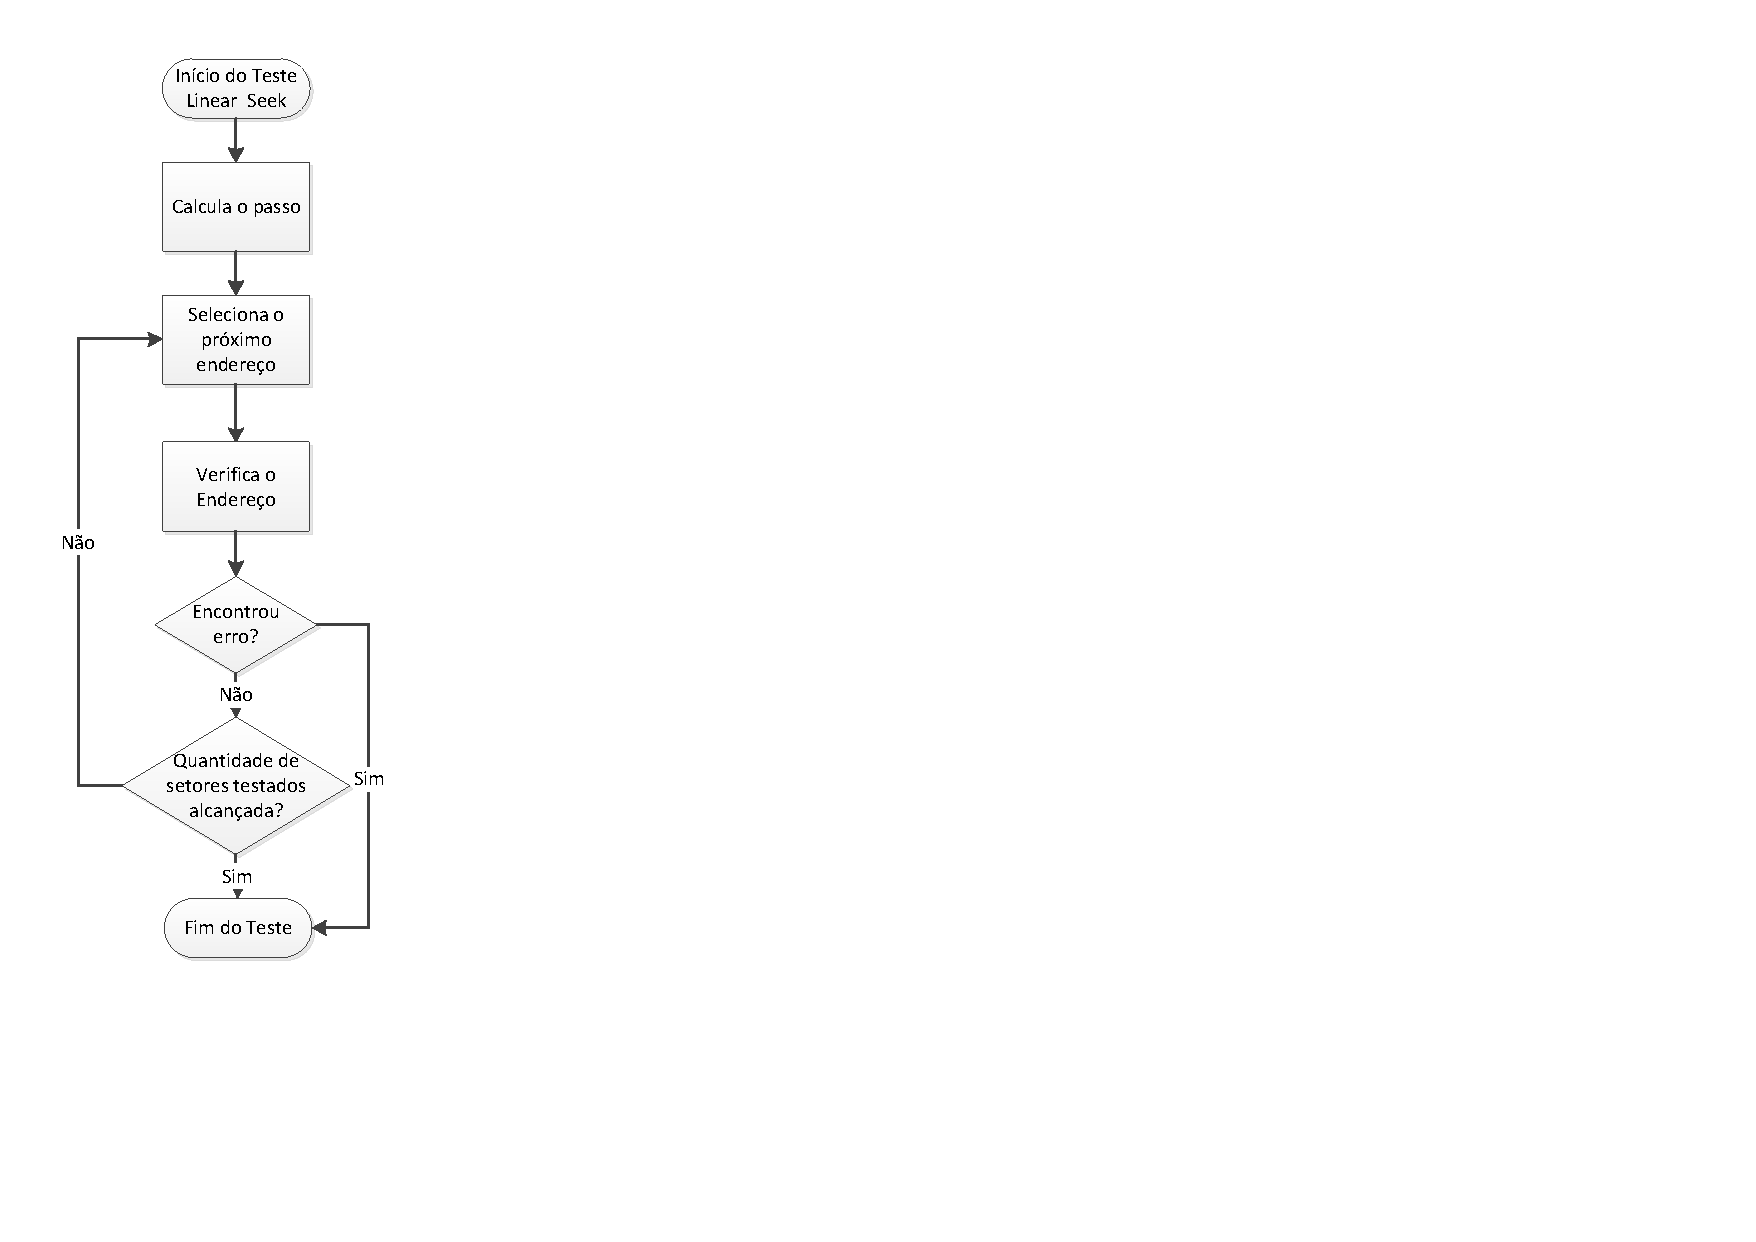
\includegraphics[width=5cm]{figs/linearseek.pdf}}
        \label{FIG:LinearSeek}
    \subfigure[b][Funnel Seek]{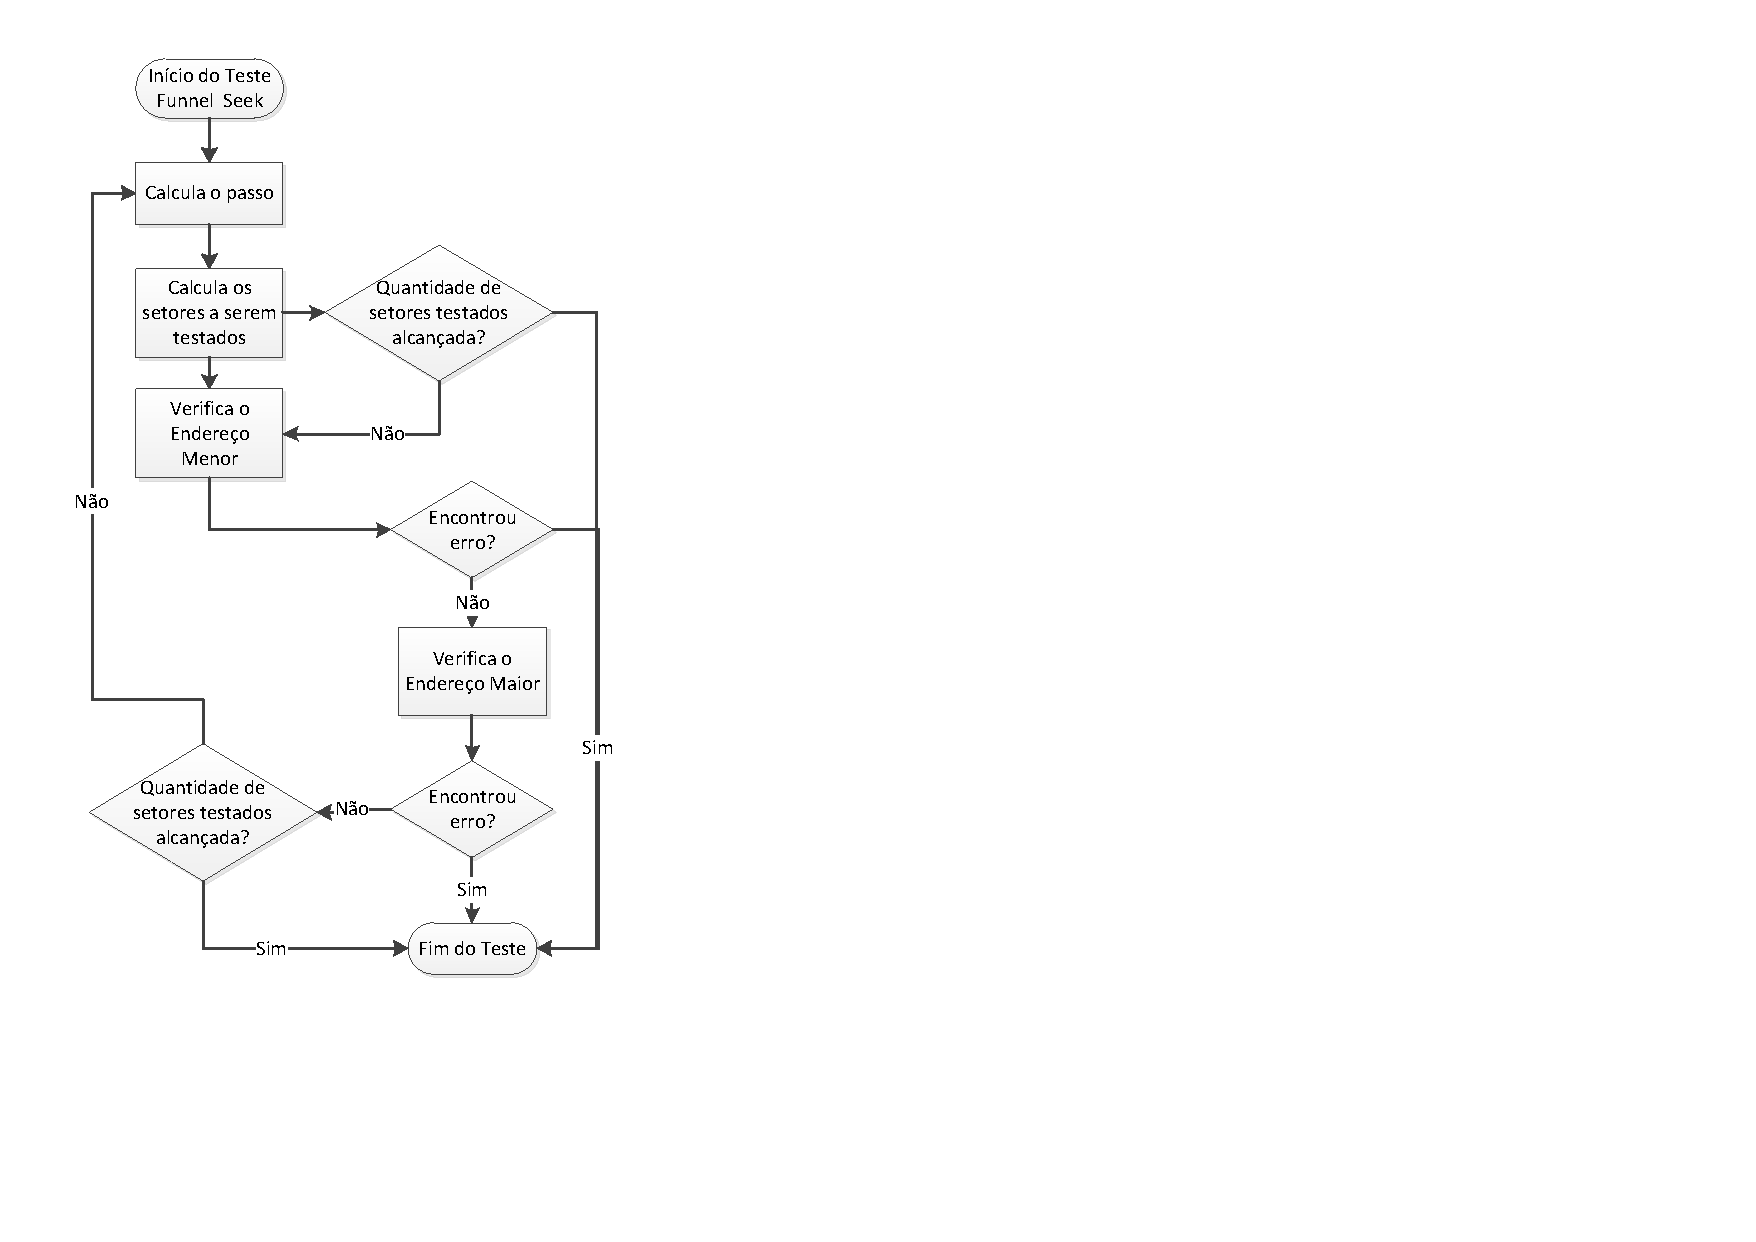
\includegraphics[width=8cm]{figs/funnelseek.pdf}}
        \label{FIG:FunnelSeek}
    \caption{Fluxograma dos algoritmos implementados: \emph{Linear e Funnel Seek}}
\end{figure}

\begin{figure}[htb!]
    \centering
\subfigure[c][Random Seek]{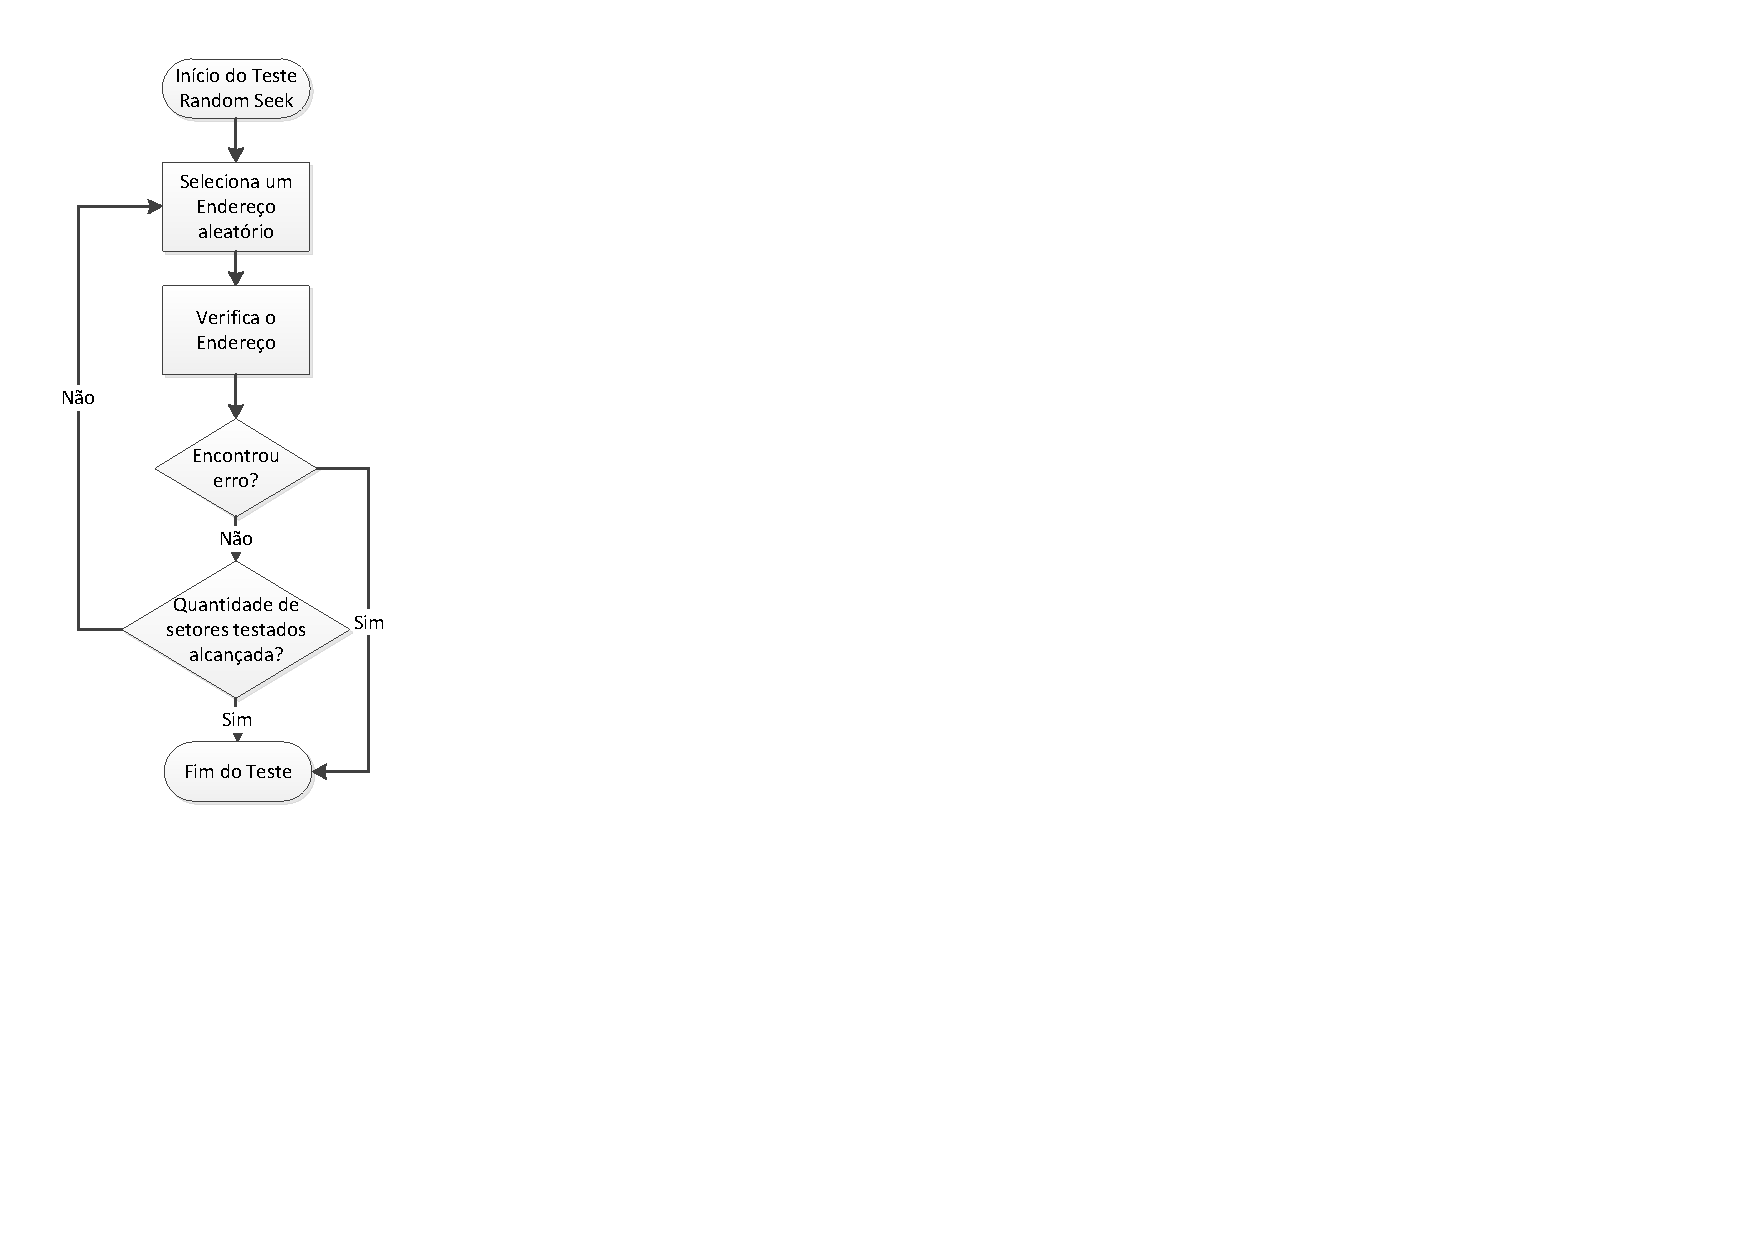
\includegraphics[width=5cm]{figs/randomseek.pdf}}
        \label{FIG:RandomSeek}
    \subfigure[d][Surface Scan]{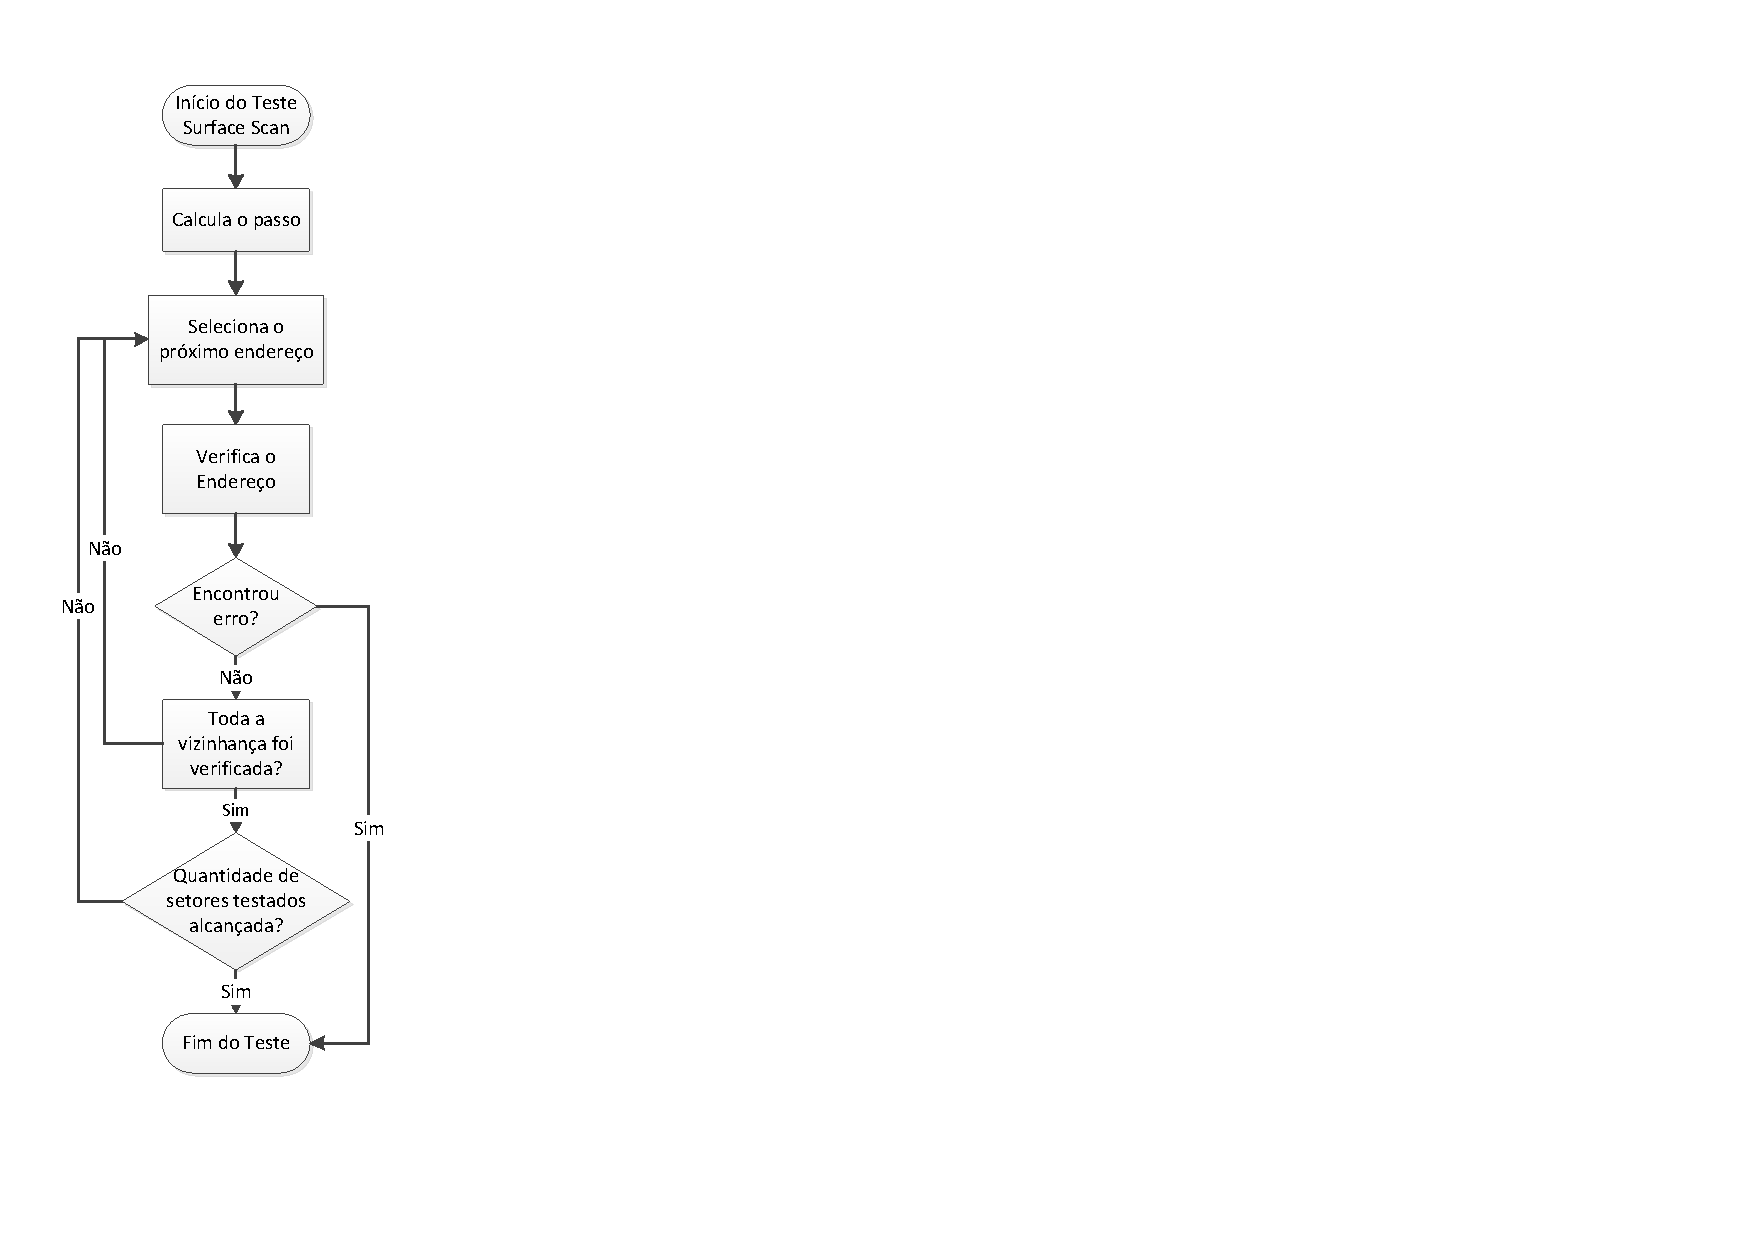
\includegraphics[width=5cm]{figs/surfacescan.pdf}}
        \label{FIG:SurfaceScan}
\caption{Fluxograma dos algoritmos implementados: \emph{Random Seek e Surface Scan}}
\end{figure}

\begin{figure}[htb!]
    \centering
    \subfigure[e][Targeted Read]{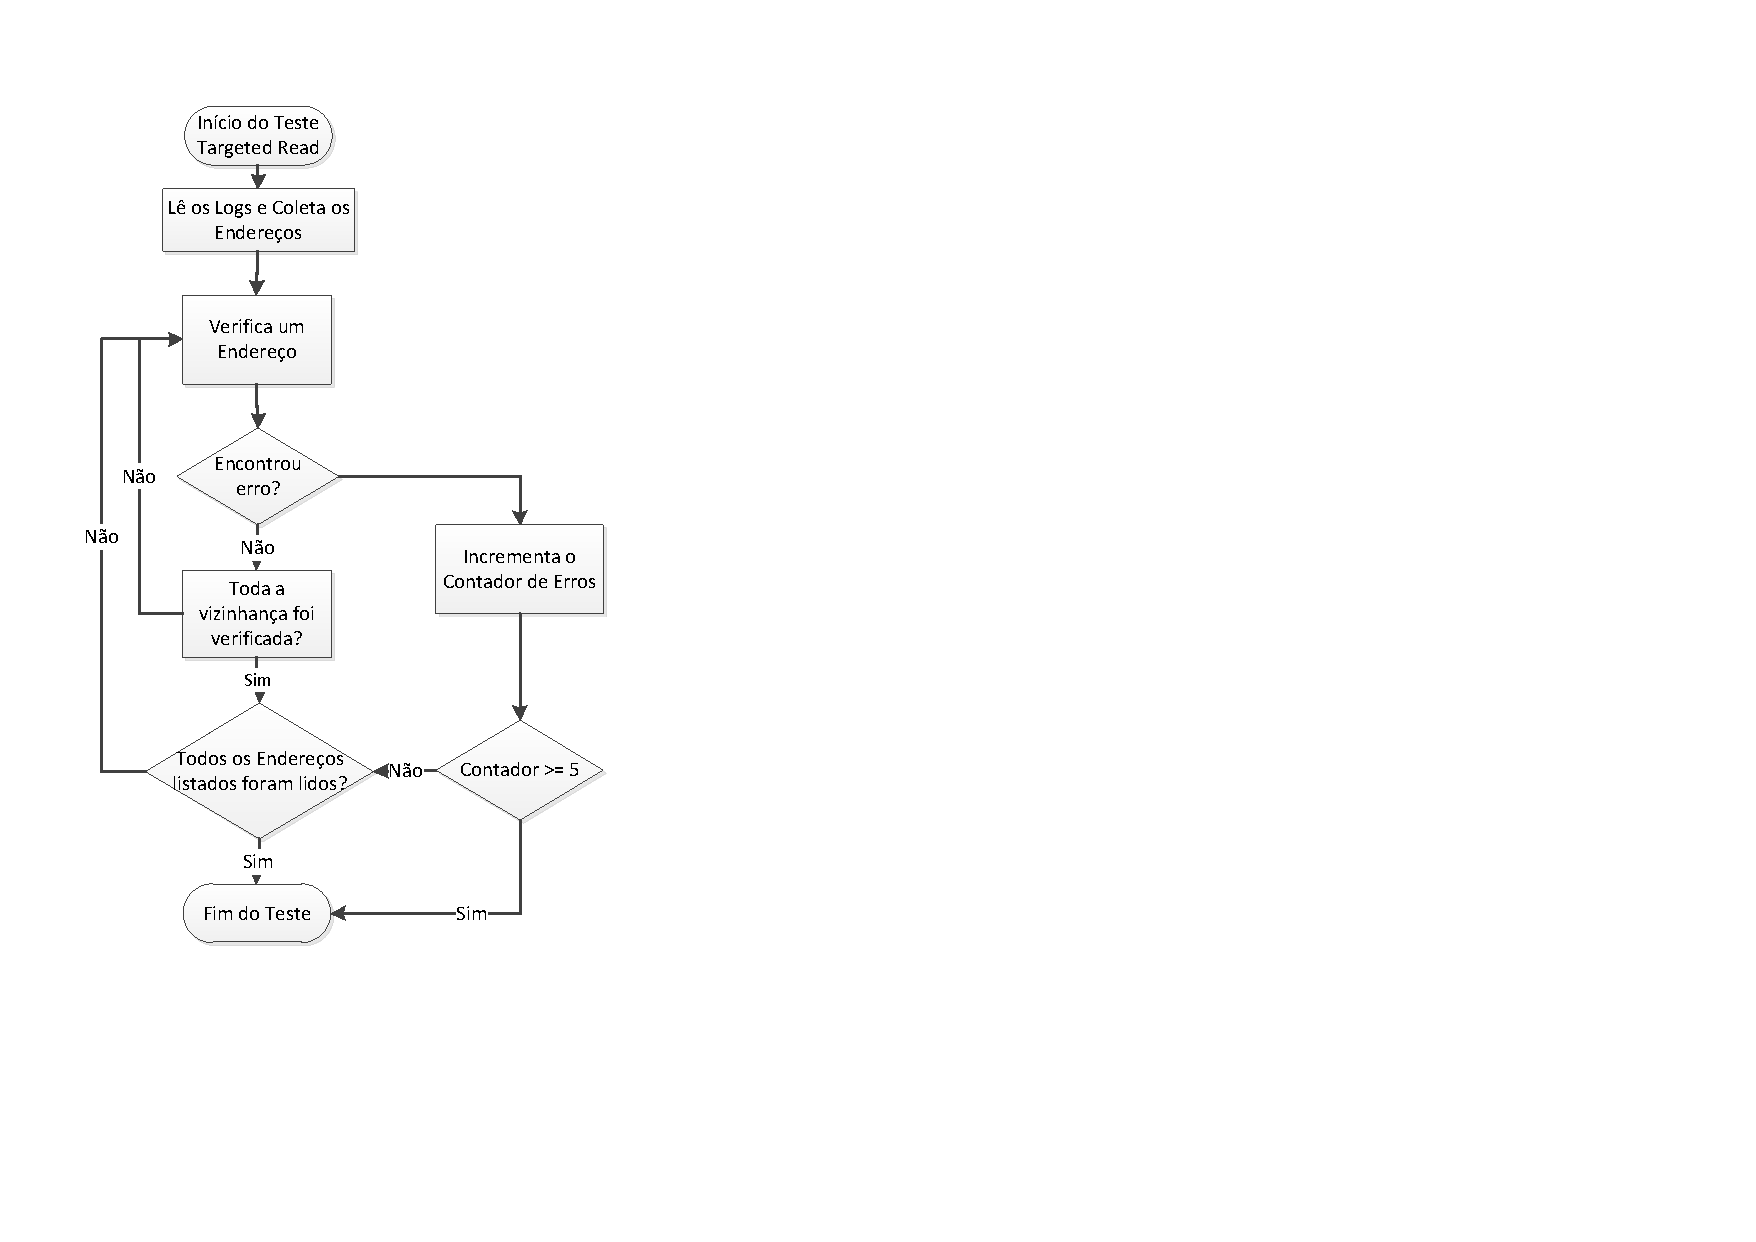
\includegraphics[width=10cm]{figs/targetedread.pdf}}
        \label{FIG:TargetedRead}
        \caption{Fluxograma dos algoritmos implementados: \emph{Targeted Read}}
\end{figure}

As quantidades de setores testadas em cada teste foram escolhidas com base no tempo m�dio de execu��o, avaliado em testes pr�-eliminares em \acp{HDD} (que s�o mais lentos que \acp{SSD}). Neste testes observou-se que o tempo m�dio para leitura de 5000 setores, em v�rios \emph{desktops} e \emph{laptops}, variava de 50 a 60 segundos, tempo pr�ximo ao observado nos \emph{softwares} do mercado para cada teste realizado.

\subsection{\emph{Bootable}}\label{bootable}

 Utilizou-se  um sistema Debian GNU/Linux para criar uma vers�o inicializ�vel do Linux.  Ele foi criado a partir de uma vers�o de 64 bits do Debian 6.0 Squeeze, kernel 2.6.32-5-amd64, usando o sistema de arquivos \emph{squashfs}. Este sistema de arquivos � somente de leitura e  implementa compress�o, sendo o mais indicado para vers�es inicializ�veis, \emph{live cd} ou \emph{pendrive} \cite{squash}.

 No total, o \emph{bootable} ocupa cerca de 200 MB e pode ser utilizado em qualquer computador que suporte inicializa��o por cd ou \emph{pendrive}. O processo de cria��o e atualiza��o do \emph{bootable} � descrito em \cite{boot:ram}. Uma ``imagem'' deste sistema de arquivos, com o Debian Squeeze instalado, foi modificada e nela o bin�rio gerado na compila��o da camada de aplica��o foi inserido. Esta nova ``imagem'' � ent�o copiada para \emph{pendrives} ou m�dias �pticas, como \acp{CD} ou \acp{DVD}, e est� pronta para ser executada.

 O bin�rio gerado na camada de aplica��o pode ser executado pelo \emph{bootable}, atrav�s da reinicializa��o do sistema, e pelo terminal, como um programa comum em outros sistemas Linux em execu��o, como Ubuntu, CentOS e outros, sem requerer reinicializa��o. Nos dois casos os par�metros s�o passados por linha de comando.

\section{Resumo do Cap�tulo}


Este cap�tulo detalhou a implementa��o do \emph{framework} e algoritmos propostos, bem como as raz�es pelos quais foram escolhidos. No pr�ximo cap�tulo os resultados do algoritmos implementados ser�o comparados com os testes de ferramentas de diagn�stico do mercado. 
%%%%%%%%%%%%%%%%%%%%%%%%%%%%%%%%%%%%%%%%%%%%%%%%%%%%%%%%%%%%%%%%%
%%%% CAP�TULO 5: Resultados
\chapter{Resultados} \label{CHP:RESULT}

Este cap�tulo aborda os resultados deste trabalho. Entre eles est�o a camada de aplica��o, os resultados obtidos a partir da metodologia descrita na Se��o \ref{metodologia}, assim como sua an�lise temporal.

\section{Camada de Aplica��o}
A implementa��o da camada de aplica��o � um programa que  compreende, al�m dos algoritmos de teste, uma interface para que o usu�rio possa execut�-los e para isso foram implementadas fun��es de listagem dos discos presentes no sistema e a filtragem para que o usu�rio possa escolher em que disco deseja realizar testes.

A Figura \ref{FIG:telainicial} mostra a interface inicial da implementa��o da camada de aplica��o. Ela cont�m o t�tulo do programa, as listagens dos algoritmos e dispositivos dispon�veis. Entre colchetes est�o os par�metros que devem ser passados para o programa durante a execu��o de cada teste. Essa figura demonstra a  execu��o do programa sem a passagem de par�metros, isso faz com que o mesmo realize a listagem das op��es dispon�veis.

\begin{figure}[htb!]
  \centering
  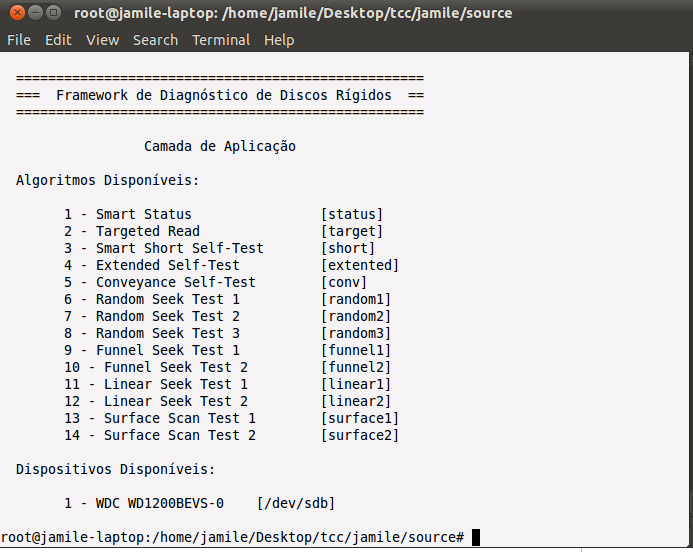
\includegraphics[scale=0.5]{figs/tela.png}
  \caption{Tela inicial da Camada de Aplica��o}
  \label{FIG:telainicial}
\end{figure}

O usu�rio pode obter informa��es sobre os par�metros esperados  executando a op��o \textbf{-h} ou \textbf{--help}.
A tela exibida durante a ajuda � mostrada na Figura \ref{FIG:telahelp}.
\begin{figure}[htb!]
  \centering
  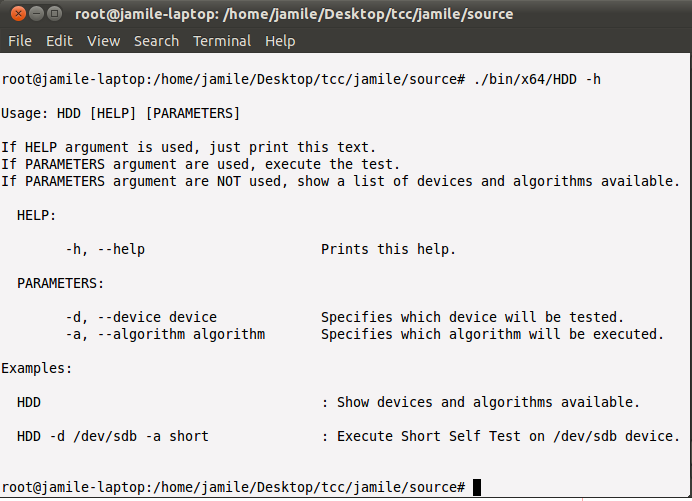
\includegraphics[scale=0.5]{figs/help.png}
  \caption{Tela de ajuda}
  \label{FIG:telahelp}
\end{figure}

A Figura \ref{FIG:telapercent} mostra um algoritmo sendo executado. Para executar um algoritmo, os seguintes par�metros devem ser passados: \textbf{-d} ou \textbf{- -device}  ``disco'' \textbf{-a} ou \textbf{- -algorithm}  ``algoritmo''. No caso da figura os par�metros passados foram: \textbf{ -d /dev/sdb -a short}. O programa ent�o passa a exibir uma barra de progresso com o percentual do teste conclu�do, qual algoritmo est� sendo executado e em que dispositivo.
\begin{figure}[htb!]
  \centering
  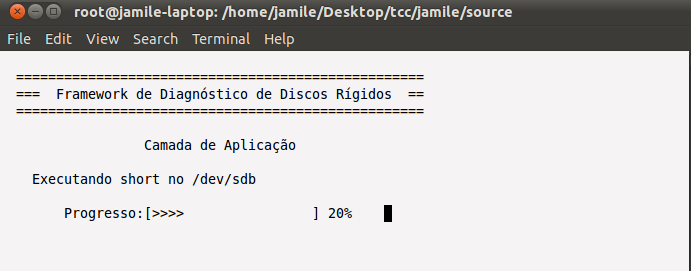
\includegraphics[scale=0.5]{figs/percent.png}
  \caption{Tela de teste em execu��o}
  \label{FIG:telapercent}
\end{figure}

Na conclus�o do teste, o tempo de execu��o � mostrado e o resultado do teste � apresentado, como mostrado na Figura \ref{FIG:telafinal}. O teste mostrado levou 120 segundos e foi conclu�do com sucesso.
\begin{figure}[htb!]
  \centering
  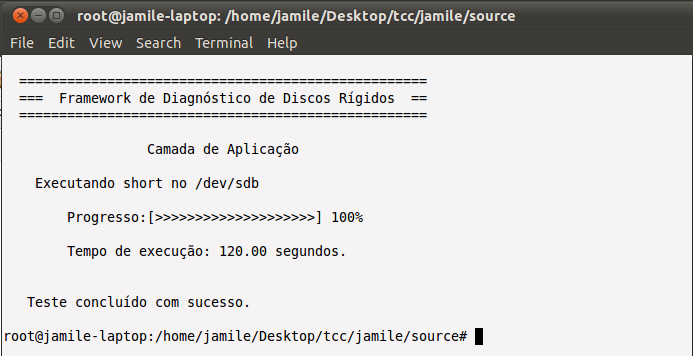
\includegraphics[scale=0.5]{figs/final.png}
  \caption{Tela de teste conclu�do}
  \label{FIG:telafinal}
\end{figure}

\section{Testes}

Nesta se��o s�o apresentados os resultados obtidos com a metodologia descrita no cap�tulo anterior. Para a realiza��o dos testes foram utilizados 12 discos r�gidos, 9 do tipo \ac{HDD} (H1, H2, H3, H4, H5, H6, H7, H8 e H9) e 3 do tipo \ac{SSD} (S1, S2 e S3), com defeitos conhecidos. Cada teste descrito nas tabelas � o resultado obtido na maior parte de 3 execu��es, ou seja, o valor apresentado se repetiu de duas a tr�s vezes.  A nota��o utilizada em todas as tabelas de resultados � descrita na Tabela \ref{TAB:not}. Na Tabela \ref{TAB:ResultsLTTFrame}, os dispositivos testados s�o listados assim como  modelos, \emph{form factors}, capacidades de armazenamento e o resultado obtido testando o dispositivo com outro \emph{software} de diagn�stico.

\begin{table}[htb!]
    \caption{Nota��o utilizada nas tabelas de resultados }
    \label{TAB:not}
    \vspace{-10pt}
    \begin{center}
      \begin{tabular}{|c|c|}
        \hline
        % after \\: \hline or \cline{col1-col2} \cline{col3-col4} ...
        Abrevia��o / S�mbolo & Defini��o \\ \hline
        $\times$ & Teste falhou \\ \hline
        $\checkmark$ & Teste passou \\ \hline
        $\emptyset$ & Teste n�o p�de ser executado \\ \hline
        Short & \ac{SMART} \emph{Short Self-Test} \\ \hline
        Status & \ac{SMART} \emph{Return Status } \\ \hline
        Conv & \ac{SMART} \emph{Conveyance Self-Test} \\ \hline
        Linear1 & \emph{Linear Seek Test 1} \\ \hline
        Linear2 & \emph{Linear Seek Test 2} \\ \hline
        Random1 & \emph{Random Seek Test 1} \\ \hline
        Random2 & \emph{Random Seek Test 2} \\ \hline
        Random3 & \emph{Random Seek Test 3} \\ \hline
        Funnel1 & \emph{Funnel Seek Test 1} \\ \hline
        Funnel2 & \emph{Funnel Seek Test 2} \\ \hline
        Surface1 & \emph{Surface Scan Test 1} \\ \hline
        Surface2 & \emph{Surface Scan Test 2} \\ \hline
        Target & \emph{Targeted Read Test} \\ \hline
      \end{tabular}
    \end{center}
    \vspace{-15pt}
\end{table}

\begin{table}[htb!]
   \caption{Lista dos dispositivos testados}
    \label{TAB:ResultsLTTFrame}
    \vspace{-10pt}
    \begin{center}
       \begin{tabular}{|c|p{5cm}|c|c|c|}
         \hline
         % after \\: \hline or \cline{col1-col2} \cline{col3-col4} ...
         Dispositivo & Modelo & Capacidade & \emph{Form Factor} & PC-Doctor \\ \hline
         H1 &  Seagate ST3500418AS & 500 GB & 3.5'' & $\checkmark$ \\ \hline
         H2 &  Western Digital WD2500AAKX083CA0 & 250GB & 3.5''&$\times$ \\ \hline
         H3 &  Seagate ST31000528AS & 1 TB &  3.5''&$\times$ \\ \hline
         H4 &  Seagate ST3500418AS & 500 GB & 2.5''& $\checkmark$ \\ \hline
         H5 &  Hitachi HTS725050A9A364 & 500 GB  &2.5''& $\times$ \\ \hline
         H6 &  Hitachi HTS545032B9A300 & 320 GB & 2.5''&$\times$ \\ \hline
         H7 & Seagate ST9250315AS & 250 GB  & 2.5''& $\times$ \\ \hline
         H8 & Toshiba MK5061GSY & 500GB &  2.5''&$\times$  \\ \hline
         H9 & Hitachi HTS723232A7A364 & 320 GB  &  2.5''&$\checkmark$   \\ \hline
         S1 & Kingston SNV425S264GB & 64 GB  & 2.5''& $\checkmark$  \\ \hline
         S2 & Toshiba THN5NC128GCSJ & 160 GB &  2.5''&$\times$ \\ \hline
         S3 & Kingston  SV100S264G& 64 GB & 2.5''& $\checkmark$  \\ \hline
       \end{tabular}
    \end{center}
    \vspace{-15pt}
\end{table}

Uma sequ�ncia de execu��o dos algoritmos foi definida com base nos \emph{softwares} do mercado e uma s�rie de hip�teses foi levantada. O primeiro questionamento � relativo � execu��o do \emph{Targeted Read Test}, teste que realiza leituras espec�ficas em regi�es onde algum tipo de problema foi detectado, a fim de determinar qual a melhor ordem de execu��o, no in�cio  ou no final  dos testes.

O segundo questionamento � em rela��o � quantidade de setores checados no algoritmo \emph{Random Seek}. Para responder a este questionamento, o desempenho de tr�s taxas distintas � avaliado.

O terceiro questionamento � quanto � validade da distin��o feita nos algoritmos de \emph{Surface Scan} e \emph{Linear Seek}. Foi avaliado se realizar os testes indo das menores para as maiores LBAs, ou das maiores para as menores LBAs, apresentam varia��es significativas de desempenho.

Por �ltimo, uma hip�tese  � levantada sobre o funcionamento do teste \emph{Funnel Seek}. Saber se, al�m da altern�ncia no sentido de ``crescimento'' da LBA analisada, a leitura de setores mais espec�ficos, como os setores iniciais do disco, que cont�m informa��es sobre a tabela de parti��o\footnote{\ac{MBR}, setor que cont�m a tabela de parti��es do disco e informa��es sobre a inicializa��o do sistema operacional, localizado no setor 0.}, pode influenciar no desempenho do algoritmo.

A ordem de execu��o dos testes definida foi: \emph{Target Read Test}, SMART \emph{Status Test}, SMART \emph{Short Self-Test}, SMART \emph{Conveyance Self-Test}, \emph{Random Seek} 1, 2 e 3, \emph{Funnel Seek} 1 e 2, \emph{Linear Seek} 1 e 2, \emph{Surface Scan} 1 e 2, e \emph{Target Read Test} e os resultados s�o apresentados na Tabela \ref{TAB:ResultsFrame}.

\begin{table}[htb!]
    \caption{Resultados dos Testes.}
    \label{TAB:ResultsFrame}
    \vspace{-10pt}
    \begin{center}
\begin{tabular}{|c|c|c|c|c|c|c|c|c|c|c|c|c|}
  \hline
  % after \\: \hline or \cline{col1-col2} \cline{col3-col4} ...
  Algoritmos & H1 & H2 & H3 & H4 & H5 & H6 & H7 & H8 & H9 & S1 & S2 & S3 \\ \hline
  Status & $\checkmark$ & $\checkmark$ & $\times$ & $\checkmark$ & $\checkmark$ & $\checkmark$ & $\checkmark$ & $\checkmark$ & $\checkmark$ & $\checkmark$  & $\checkmark$ & $\checkmark$ \\ \hline
  Short & $\checkmark$ & $\times$ & $\times$ & $\checkmark$ & $\times$  & $\checkmark$  & $\times$  & $\times$  & $\checkmark$  & $\checkmark$  & $\times$ & $\checkmark$ \\ \hline
  Conv & $\checkmark$  & $\times$ & $\times$ & $\checkmark$ & $\emptyset$ & $\emptyset$ &$\times$ & $\emptyset$ & $\emptyset$ & $\emptyset$ & $\emptyset$ & $\emptyset$ \\ \hline
  Random1 & $\checkmark$  & $\checkmark$  & $\checkmark$  & $\checkmark$  & $\checkmark$  & $\checkmark$  & $\checkmark$  & $\checkmark$  & $\checkmark$  & $\checkmark$  & $\checkmark$ & $\checkmark$ \\ \hline
  Random2 & $\checkmark$  & $\checkmark$  & $\checkmark$  & $\checkmark$  & $\times$  & $\checkmark$  & $\checkmark$  & $\checkmark$  & $\checkmark$  & $\checkmark$  & $\checkmark$ & $\checkmark$ \\ \hline
  Random3 & $\checkmark$  & $\checkmark$  & $\checkmark$  & $\checkmark$  & $\times$  & $\checkmark$  & $\checkmark$  & $\checkmark$  & $\checkmark$  & $\checkmark$  & $\checkmark$ & $\checkmark$ \\ \hline
  Funnel1 & $\checkmark$  & $\checkmark$   & $\checkmark$  & $\checkmark$  & $\checkmark$  & $\checkmark$  & $\times$  & $\checkmark$  & $\checkmark$  & $\checkmark$  & $\checkmark$ & $\checkmark$ \\ \hline
  Funnel2 & $\checkmark$  & $\times$  & $\checkmark$  & $\checkmark$  & $\times$  & $\checkmark$  & $\times$  & $\checkmark$  & $\checkmark$  & $\checkmark$  & $\checkmark$ & $\checkmark$ \\ \hline
  Linear1 & $\checkmark$  & $\checkmark$  & $\checkmark$  & $\checkmark$  & $\checkmark$  & $\checkmark$  & $\checkmark$  & $\checkmark$  & $\checkmark$  & $\checkmark$  & $\checkmark$ & $\checkmark$ \\ \hline
  Linear2 & $\checkmark$  & $\checkmark$  & $\checkmark$  & $\checkmark$  & $\checkmark$  & $\checkmark$  & $\checkmark$  & $\checkmark$  & $\checkmark$  & $\checkmark$  & $\checkmark$ & $\checkmark$ \\ \hline
  Surface1 & $\checkmark$ & $\times$ & $\checkmark$ & $\checkmark$ & $\checkmark$ & $\checkmark$ & $\checkmark$ & $\checkmark$ & $\checkmark$ & $\checkmark$  & $\checkmark$ & $\checkmark$ \\ \hline
  Surface2 & $\checkmark$ & $\times$ & $\checkmark$ & $\checkmark$ & $\checkmark$ & $\checkmark$ & $\checkmark$ & $\times$ & $\checkmark$ & $\checkmark$  & $\checkmark$ & $\checkmark$ \\ \hline
  Target   & $\checkmark$ & $\times$ & $\checkmark$ & $\checkmark$ & $\times$ & $\times$ & $\times$ & $\times$ & $\checkmark$  & $\checkmark$  & $\times$ & $\checkmark$ \\
  \hline
  \end{tabular}
    \end{center}
    \vspace{-15pt}
\end{table}

Os melhores resultados obtidos individualmente foram \emph{SMART Short Self-Test} e \emph{Targeted Read Test}, que detectaram 6 dos 7 dispositivos com falhas. Depois destes est�o o \emph{Funnel Seek 2} e o  \emph{SMART Conveyance Self-Test}, que detectaram sozinhos 3 dos 7 dispositivos falhos. Entretanto, vale salientar que o \emph{SMART Conveyance Self-Test} n�o pode ser executado na maioria dos dispositivos, pois estes n�o t�m suporte a este tipo de teste. Em seguida est� o \emph{Surface Scan 2}, que detectou 2 dos 7 dispositivos falhos e os testes  \emph{Random Seek 2}, \emph{Random Seek 3}, \emph{Funnel Seek 1} e  \emph{Surface Scan 1} que detectaram apenas 1 dos 7 dispositivos falhos. Por �ltimo, est�o  \emph{Random Seek 1}, \emph{Linear Seek 1} e \emph{Linear Seek 2}, que n�o detectaram nenhum dispositivo falho. O alerta de falha dado pelo \emph{SMART Return Status} foi dado apenas para 1 dispositivo e em nenhum dos testes foi observado resultados ``falsos positivos''.

H� importantes pontos a serem analisados. Das tr�s rodadas de testes executadas, a primeira apresentou resultados diferentes entre a execu��o do \emph{Targeted Read Test} no in�cio e no final dos testes. A execu��o inicial detectou apenas 3 dos 7 dispositivos com falhas. Depois da execu��o dos demais testes o \emph{Targeted Read Test} passou a detectar 6 dos 7 dispositivos com falha. Este resultado, da execu��o final, se repetiu nas duas execu��es de cada uma das duas rodadas seguintes. Logo, para o usu�rio � interessante que este teste seja o �ltimo a ser executado.

Este comportamento do \emph{Targeted Read Test} pode ser explicado pela leitura dos \emph{logs} da controladora. Quando outros testes s�o executados, setores com falha podem ser detectados ou, mesmo que o teste n�o seja reprovado, qualquer comportamento estranho que tenha ocorrido ser� registrado no \emph{log} e posteriormente verificado com o \emph{Targeted Read Test}.

 O \emph{Random Seek Test} apresentou baixo desempenho na detec��o de dispositivos com falha, apenas os testes 2 e 3 detectaram 1 dos 7 dispositivos falhos. Entretanto, o desempenho dos algoritmos deve ser analisado conjuntamente e como se trata de um algoritmo fundamentado em aleatoriedade, a realiza��o destes testes com outro conjunto de dispositivos pode apresentar resultados vari�veis.

 Os algoritmos de \emph{Linear Seek} e \emph{Surface Scan} n�o se mostraram eficientes independentemente da ordem de ``crescimento'' das LBAs analisadas, se da menor para a maior ou o contr�rio.

 Um desempenho interessante foi o do \emph{Funnel Seek Test 2}, que se mostrou significativamente melhor que o \emph{Funnel Seek 1}, lembrando que a diferen�a entre eles � a checagem dos 100 primeiros setores do disco feita pelo \emph{Funnel Seek Test 2}.

De maneira geral, o conjunto dos 13 testes implementados foi capaz de detectar os 7 dispositivos defeituosos, alcan�ando assim o resultado obtido utilizando o PC-Doctor.

\section{Tempo de Execu��o}

 Al�m da cobertura de falhas, o tempo de execu��o dos testes deve ser analisado. Na Tabela \ref{TAB:TimeFrame}, s�o apresentados os tempos de execu��o da �ltima rodada dos testes.
\begin{table}[htb!]
    \caption{Tempos de Execu��o dos Testes, em segundos.}                                                                                                         \label{TAB:TimeFrame}
    \vspace{-10pt}
    \begin{center}
\begin{tabular}{|c|c|c|c|c|c|c|c|c|c|c|c|c|}
  \hline
  % after \\: \hline or \cline{col1-col2} \cline{col3-col4} ...
  Algoritmos & H1 & H2 & H3 & H4 & H5 & H6 & H7 & H8 & H9 & S1 & S2 & S3 \\ \hline
  Status & 0 & 1 & 0 & 0 & 0 & 0 & 14 &  0 & 0 & 0  & 1 & 0 \\ \hline
  Short & 81 & 10 & 10 & 60 & 50  & 120  & 24 & 41  &  120  & 50  & 11 & 50 \\ \hline
   Conv & 140  &10 & 10 & 121 & - & - & 24 & -&   - & - & - & - \\ \hline
   Random1 & 106  & 82  & 107  & 106  & 126  & 131  &114  & 83  & 137  & 3  & 1& 1 \\ \hline
   Random2 & 159  & 123  & 162  & 160  & 192  & 196  & 163  &  125 & 205  & 4  & 3 & 2 \\ \hline
   Random3 & 214  & 163  & 250  & 213  & 192  & 262  & 213  &  166  & 274  & 6  & 4 & 4 \\ \hline
   Funnel1 & 129  & 52   & 524  & 129  & 150  & 101  & 18  & 103 & 104  & 0  & 0 & 0 \\ \hline
   Funnel2 & 131  & 52  & 400  & 130  & 150  & 102  & 19  & 104  & 106  & 0  & 1 & 1 \\ \hline
   Linear1 & 49  & 31  & 52  & 47  & 71  & 84 & 67  & 43 &  89  & 3  &2 & 2\\ \hline
   Linear2 & 48  & 32  & 52  & 48  & 72  & 84 & 66  & 44  &  89  & 3  & 2 & 2 \\ \hline
   Surface1 & 535 & 7 & 541 & 533 & 848 & 872 & 677 &  501 & 972 & 36  & 19 & 19 \\ \hline
   Surface2 & 536 & 71 & 543 & 533 & 852 & 873 & 678 &  204 & 968 & 36 & 19 & 19 \\ \hline
   Target   & 1 & 27 & 0 & 0 & 32 & 24 & 10 & 14 &  1  & 0 & 0 & 0 \\                                                                                   \hline                                                                                                                                   \end{tabular}                                                                                                                            \end{center}                                                                                                                       \vspace{-15pt}
\end{table}

Na tabela h� duas grandes ``discrep�ncias'' de tempo: a primeira ocorre entre o tempo levado para executar os testes em dispositivos SSD e a segunda ocorre quando uma falha � encontrada. Neste caso, em uma leitura normal leva-se um tempo maior para o resultado da leitura, pois v�rias tentativas s�o feitas. Entretanto, quando um setor falho � encontrado, a condi��o de parada do algoritmo � satisfeita e ele � encerrado. Como no teste de \emph{Surface Scan 1} do H2, que durou 7 segundos, enquanto que o mesmo teste para o H1, que tem o dobro da capacidade, levou 535 segundos, por exemplo.

 Os testes mais r�pidos foram os de \emph{SMART Return Status} e \emph{Targeted Read}. Em v�rios dispositivos a execu��o levou menos de 1 segundo. Entre os testes de \emph{Random Seek} os testes variaram de 82  a 274 segundos para \acp{HDD} e entre 1 e 6 para \acp{SSD}. Os testes mais demorados foram os de \emph{Surface Scan}, chegando a durar 972 segundos, como no caso do H9. Na Figura \ref{FIG:Tempo_medio}, o tempo m�dio em segundos de cada teste realizado em dispositivos \ac{HDD} (mais demorados) � apresentado.

\begin{figure}[htb]
  \centering
  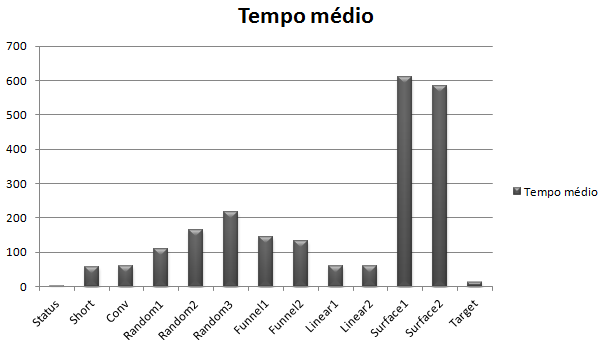
\includegraphics[scale=0.8]{figs/tempo_medio.png}
  \caption{Tempo m�dio dos testes para dispositivos HDD}
  \label{FIG:Tempo_medio}
\end{figure}

Uma sele��o de algoritmos foi feita com base na an�lise dos resultados dos testes e dos tempos de execu��o. Os cinco algoritmos selecionados foram: \emph{SMART Return Status}, \emph{SMART Short Self-Test}, \emph{Random Seek Test 2}, \emph{Funnel Seek Test 2} e \emph{Target Read Test}. Considerando apenas esta combina��o de algoritmos foi poss�vel detectar todos os dispositivos com falha e a soma dos tempos de execu��o foi inferior aos 10 minutos colocados como objetivo para a execu��o de um teste r�pido e eficiente no diagn�stico de discos r�gidos. Na Tabela \ref{TAB:CompFramePCDoc}, os resultados obtidos com esta sele��o de algoritmos e o PC-Doctor foram comparados. Todos os dispositivos defeituosos detectados pelo PC-Doctor tamb�m foram detectados pela sele��o de algoritmos.

\begin{table}[htb!]
    \caption{Compara��o dos Resultados obtidos com a sele��o de algoritmos e o PC-Doctor.}
    \label{TAB:CompFramePCDoc}
    \vspace{-10pt}
    \begin{center}
\begin{tabular}{|c|c|c|c|c|c|c|c|c|c|c|c|c|}
\hline
  % after \\: \hline or \cline{col1-col2} \cline{col3-col4} ...
  Algoritmos & H1 & H2 & H3 & H4 & H5 & H6 & H7 & H8 & H9 & S1 & S2 & S3 \\ \hline
   \hline\hline
  Framework & $\checkmark$ & $\times$ & $\times$ & $\checkmark$ & $\times$ & $\times$ & $\times$ & $\times$ & $\checkmark$  & $\checkmark$  & $\times$ & $\checkmark$ \\
  \hline\hline
  PC-Doctor & $\checkmark$ & $\times$ & $\times$ & $\checkmark$ & $\times$ & $\times$ & $\times$ & $\times$ & $\checkmark$  & $\checkmark$  & $\times$ & $\checkmark$ \\
  \hline \hline
  \end{tabular}
    \end{center}
    \vspace{-15pt}
\end{table}

O \emph{SMART Return Status} foi escolhido por ser um importante sinalizador  da ``sa�de'' do dispositivo. O \emph{SMART Short Self-Test} e o \emph{Target Read Test} foram escolhidos por terem apresentado a melhor capacidade de detec��o de falhas  entre os algoritmos avaliados. Por fim,  o \emph{Random Seek Test 2} e o \emph{Funnel Seek Test 2} foram escolhidos por terem apresentado uma capacidade mediana de detec��o e  servirem de complemento ao \emph{Target Read Test}.

\section{Resumo do Cap�tulo}

Neste cap�tulo foram apresentados os resultados obtidos no desenvolvimento do \emph{Framework} proposto: a cria��o de um programa capaz de executar testes de diagn�stico e que possibilitou a an�lise de algoritmos de teste  e a sele��o dos algoritmos mais eficientes com base na an�lise realizada.

No pr�ximo cap�tulo s�o apresentadas as conclus�es e propostas de continua��o deste trabalho. 
%%%%%%%%%%%%%%%%%%%%%%%%%%%%%%%%%%%%%%%%%%%%%%%%%%%%%%%%%%%%%%%%%
%%%% CAP�TULO 5: Conclus�es
\chapter{Conclus�o}

Neste trabalho foi desenvolvido um \emph{framework} para dar suporte ao desenvolvimento de testes de diagn�stico de discos r�gidos usados em computadores pessoais. Utilizou-se o sistema Linux pois, mesmo sendo empregado  por uma pequena parcela do mercado, possibilita a realiza��o de testes em computadores com qualquer sistema operacional instalado, bastando apenas a reinicializa��o.

O programa desenvolvido com a camada de aplica��o, criada utilizando o \emph{framework} apresentado neste trabalho, mostrou-se bastante eficiente pois apresentou desempenho similar aos das ferramentas de diagn�stico do mercado. Todos os dispositivos com falhas foram detectados, utilizando apenas uma combina��o de 5 testes, com tempo de execu��o inferior a 10 minutos.

Entretanto, a maior contribui��o deste trabalho est� n�o apenas na an�lise realizada da efici�ncia dos algoritmos de testes, mas em  fornecer os recursos necess�rios para  a implementa��o de novos algoritmos de maneira simples, como os principais comandos necess�rios, uma camada de aplica��o que encapsula estes comandos e um m�todo de inser��o de falhas, �til na valida��o de novos comandos e algoritmos de teste.

Durante o desenvolvimento deste trabalho, algumas dificuldades foram enfrentadas, principalmente devido � documenta��o dos padr�es \ac{ATA} e \ac{SCSI}, que se mostrou superficial e mal organizada. H� livros que se dedicam a fazer uma an�lise mais detalhada destes padr�es, entretanto os mesmos s�o antigos e est�o um pouco defasados. Para contornar este empecilho, v�rios testes e experimentos foram realizados para tentar deduzir, atrav�s de investiga��o, o comportamento que n�o era descrito pela documenta��o.

\section{Perspectivas Futuras}


Este trabalho pode ser continuado de diversas maneiras. Pode-se trabalhar na implementa��o de mais comandos \ac{SCSI}, visando dar cobertura tamb�m a discos \ac{SAS} e a servidores. A interface gr�fica deve ser aprimorada, para que se torne mais robusta e mais  agrad�vel de ser utilizada. Por fim, a principal vertente de continua��o deste trabalho � o  desenvolvimento de novos algoritmos e o aprimoramento dos testes implementados aqui, com a realiza��o de mais rodadas de teste e a experimenta��o de novos par�metros em um conjunto maior de discos r�gidos.


%%%%%%%%%%%%%%%%%%%%%%%%%%%%%%%%%%%%%%%%%%%%%%%%%%%%%%%%%%%%%%%%%
%%% AP\^{E}NDICE
%\appendix
%\begin{appendices}
%\chapter{Exemplo Comando Inquiry} \label{APX:ATA}

MATS:

\begin{table}[!ht]
\caption{\emph{MATS.}}
\centering
\label{TAB:MATS}
\begin{tabular}{| c | l r |}
\hline
1 & W0 & $\Updownarrow$ \\
2 & R0, W1 & $\Updownarrow$ \\
3 & R1 & $\Updownarrow$ \\
\hline
\end{tabular}
\end{table}


%%\chapter{Cria��o de Bootable} \label{APX:SCSI}

\begin{verbatim}
Customize Live Environment

This procedure is almost identical to customizing a LiveCD (up to the generation of the .squashfs image). Please see LiveCDCustomization for detailed instructions on customizing the LiveCD. I will only be providing a basic rundown on the process.

Extract /casper/filesystem.squashfs to /casper/chroot/

sudo mount -o loop -t squashfs /casper/filesystem.squashfs /mnt
sudo mkdir /casper/chroot
sudo rsync -ax /mnt/. /casper/chroot/.
sudo umount /mnt
Regenerate initrd.gz
Since we edited bootup scripts, we need to regenerate the file we know as /casper/initrd.gz to incorporate these changes:


sudo cp -L /etc/resolv.conf /casper/chroot/etc/
sudo mount -t proc none /casper/chroot/proc
sudo mount -o bind /dev /casper/chroot/dev
sudo chroot /casper/chroot /bin/bash
At this point, you are "in" the live environment's filesystem. We will be doing this a few more times before the day is over. Remember that our Live environment is at /casper/chroot, not at edit/ (adjust customization commands accordingly).

Optional: Customize Live Environment Further

It would be a great idea to add or remove some packages, or add some default user settings, etc, to make the live environment friendlier. The previously linked LiveCD customization article provides full details on how to do a wide variety of customizations. Follow those instructions, up to: "Putting the CD together" (don't do that step). Instead, replace it with

Ideas for customizations specific to this howto include:

Removing behemoth packages like OpenOffice.

Adding proprietary 3D video drivers by default (TODO: expand on this idea)
Removing shutdown scripts (TODO: expand)
Customizing user default settings in /etc/skel, including importing a firefox profile, etc. The LiveCD howto roughly states how to do this. (TODO: expand)
Suppress the eject notice at shutdown.

rm /etc/rc?.d/*casper*
Install something like sshfs so you can easily use SSH-able systems as permanent storage (TODO: Expand)
Upgrade the whole system and regenerate initrd.gz


apt-get update
apt-get dist-upgrade
apt-get autoclean
apt-get autoremove
apt-get clean
mkinitramfs -o /new-initrd.gz 2.6.31-16-generic
exit
umount -l /casper/chroot/dev
umount -l /casper/chroot/proc
The mkinitramfs command may take 30 seconds to a few minutes, depending on your CPU speed. The exit command will take you back to your original shell, that's not within with live environment. Now we will move this initrd to the right spot:


sudo mv /casper/chroot/new-initrd.gz /casper/initrd.gz
sudo mksquashfs /casper/chroot /casper/filesystem.squashfs -noappend -always-use-fragments
The always-use-fragments argument allows space to be used more efficiently, at the cost of more seeking. Since our image is to be loaded into RAM, seeking is costless and not a concern as opposed to on a mechanical medium.


title Jaunty RAM Session
kernel /casper/vmlinuz boot=casper toram splash
initrd /casper/initrd.gz
Reboot and Enjoy


\end{verbatim}
%
%\begin{verbatim}
%    D - Direct Access Block Device (SBC-3)            Device Column key
%    .T - Sequential Access Device (SSC-3)             ---------------------
%    . L - Printer Device (SSC)                        M = Mandatory
%    .  P - Processor Device (SPC-2)                   O = Optional
%    .  .W - Write Once Block Device (SBC)             V = Vendor specific
%    .  . R - C/DVD Device (MMC-6)                     Z = Obsolete -- with
%    .  .  O - Optical Memory Block Device (SBC)           [std] identifying
%    .  .  .M - Media Changer Device (SMC-3)               last standard
%    .  .  . A - Storage Array Device (SCC-2)
%    .  .  .  E - SCSI Enclosure Services device (SES-2)
%    .  .  .  .B - Simplified Direct-Access (Reduced Block) device (RBC)
%    .  .  .  . K - Optical Card Reader/Writer device (OCRW)
%    .  .  .  .  V - Automation/Device Interface device (ADC-2)
%    .  .  .  .  .F - Object-based Storage Device (OSD-2)
%    .  .  .  .  .
%OP  DTLPWROMAEBKVF  Description
%00  MMMMMMMMMMMMMM  TEST UNIT READY
%01   M              REWIND
%01  Z V ZZZZ        REZERO UNIT [SBC]
%02  VVVVVV V
%03  MMMMMMMMMMOMMM  REQUEST SENSE
%04  M    OO         FORMAT UNIT
%%04   O              FORMAT MEDIUM
%%OP  DTLPWROMAEBKVF  Description
%%04    O             FORMAT
%%05  VMVVVV V        READ BLOCK LIMITS
%%06  VVVVVV V
%%07  OVV O OV        REASSIGN BLOCKS
%%07         O        INITIALIZE ELEMENT STATUS
%%08  MMV O OV        READ(6)
%%08     O            RECEIVE
%%08                  GET MESSAGE(6)
%%09  VVVVVV V
%%0A  OO  O OV        WRITE(6)
%%0A     M            SEND(6)
%%0A                  SEND MESSAGE(6)
%%0A    M             PRINT
%%0B  Z   ZOZV        SEEK(6) [SBC]
%%0B   O              SET CAPACITY
%%0B    O             SLEW AND PRINT
%%0C  VVVVVV V
%%0D  VVVVVV V
%%0E  VVVVVV V
%%0F  VOVVVV V        READ REVERSE(6)
%%10  VM VVV          WRITE FILEMARKS(6)
%%10    O             SYNCHRONIZE BUFFER
%%11  VMVVVV          SPACE(6)
%%12  MMMMMMMMMMMMMM  INQUIRY
%%13  V VVVV
%%13   O              VERIFY(6)
%%14  VOOVVV          RECOVER BUFFERED DATA
%%15  OMO O OOOO OO   MODE SELECT(6)
%%16  ZZMZO OOOZ O    RESERVE(6) [SPC-2]
%%16         Z        RESERVE ELEMENT(6) [SMC]
%%17  ZZMZO OOOZ O    RELEASE(6) [SPC-2]
%%17         Z        RELEASE ELEMENT(6) [SMC]
%%18  ZZZZOZO    Z    COPY [SPC]
%%19  VMVVVV          ERASE(6)
%%OP  DTLPWROMAEBKVF  Description
%%1A  OMO O OOOO OO   MODE SENSE(6)
%%1B  O   OOO O MO O  START STOP UNIT
%%1B   O          M   LOAD UNLOAD
%%1B                  SCAN
%%1B    O             STOP PRINT
%%1B         O        OPEN/CLOSE IMPORT/EXPORT ELEMENT
%%1C  OOOOO OOOM OOO  RECEIVE DIAGNOSTIC RESULTS
%%1D  MMMMM MMOM MMM  SEND DIAGNOSTIC
%%1E  OO  OOOO   O O  PREVENT ALLOW MEDIUM REMOVAL
%%1F
%%20  V   VVV    V
%%21  V   VVV    V
%%22  V   VVV    V
%%23  V   V V    V
%%23       O          READ FORMAT CAPACITIES
%%24  V   VV          SET WINDOW
%%25  M   M M   M     READ CAPACITY(10)
%%25       O          READ CAPACITY
%%25             M    READ CARD CAPACITY
%%25                  GET WINDOW
%%26  V   VV
%%27  V   VV
%%28  M   MOM   MM    READ(10)
%%28                  GET MESSAGE(10)
%%29  V   VVO         READ GENERATION
%%2A  O   MOM   MO    WRITE(10)
%%2A                  SEND(10)
%%2A                  SEND MESSAGE(10)
%%2B  Z   OOO    O    SEEK(10) [SBC]
%%2B   M              LOCATE(10)
%%2B         O        POSITION TO ELEMENT
%%2C  V    OO         ERASE(10)
%%2D        O         READ UPDATED BLOCK
%%2D  V
%%OP  DTLPWROMAEBKVF  Description
%%2E  O   OOO   MO    WRITE AND VERIFY(10)
%%2F  O   OOO         VERIFY(10)
%%30  Z   ZZZ         SEARCH DATA HIGH(10) [SBC]
%%31  Z   ZZZ         SEARCH DATA EQUAL(10) [SBC]
%%31                  OBJECT POSITION
%%32  Z   ZZZ         SEARCH DATA LOW(10) [SBC]
%%33  Z   OZO         SET LIMITS(10) [SBC]
%%34  O   O O    O    PRE-FETCH(10)
%%34   M              READ POSITION
%%34                  GET DATA BUFFER STATUS
%%35  O   OOO   MO    SYNCHRONIZE CACHE(10)
%%36  Z   O O    O    LOCK UNLOCK CACHE(10) [SBC]
%%37  O     O         READ DEFECT DATA(10)
%%37         O        INITIALIZE ELEMENT STATUS WITH RANGE
%%38      O O    O    MEDIUM SCAN
%%39  ZZZZOZO    Z    COMPARE [SPC]
%%3A  ZZZZOZO    Z    COPY AND VERIFY [SPC]
%%3B  OOOOOOOOOOMOOO  WRITE BUFFER
%%3C  OOOOOOOOOO OOO  READ BUFFER
%%3D        O         UPDATE BLOCK
%%3E  O   O O         READ LONG(10)
%%3F  O   O O         WRITE LONG(10)
%%OP  DTLPWROMAEBKVF  Description
%%40  ZZZZOZOZ        CHANGE DEFINITION [SPC]
%%41  O               WRITE SAME(10)
%%42  O               UNMAP
%%42       O          READ SUB-CHANNEL
%%43       O          READ TOC/PMA/ATIP
%%44   M          M   REPORT DENSITY SUPPORT
%%44                  READ HEADER
%%45       O          PLAY AUDIO(10)
%%46       M          GET CONFIGURATION
%%47       O          PLAY AUDIO MSF
%%48  O         O     SANITIZE
%%OP  DTLPWROMAEBKVF  Description
%%49
%%4A       M          GET EVENT STATUS NOTIFICATION
%%4B       O          PAUSE/RESUME
%%4C  OOOOO OOOO OOO  LOG SELECT
%%4D  OOOOO OOOO OMO  LOG SENSE
%%4E       O          STOP PLAY/SCAN
%%4F
%%50  O               XDWRITE(10)
%%51  O               XPWRITE(10)
%%51       O          READ DISC INFORMATION
%%52  O               XDREAD(10)
%%52       O          READ TRACK INFORMATION
%%53  O               XDWRITEREAD(10)
%%53       O          RESERVE TRACK
%%54       O          SEND OPC INFORMATION
%%55  OOO OMOOOOMOMO  MODE SELECT(10)
%%56  ZZMZO OOOZ      RESERVE(10) [SPC-2]
%%56         Z        RESERVE ELEMENT(10) [SMC]
%%57  ZZMZO OOOZ      RELEASE(10) [SPC-2]
%%57         Z        RELEASE ELEMENT(10) [SMC]
%%58       O          REPAIR TRACK
%%59
%%5A  OOO OMOOOOMOMO  MODE SENSE(10)
%%5B       O          CLOSE TRACK/SESSION
%%5C       O          READ BUFFER CAPACITY
%%5D       O          SEND CUE SHEET
%%5E  OMOOO OOOO   M  PERSISTENT RESERVE IN
%%5F  OMOOO OOOO   M  PERSISTENT RESERVE OUT
%%7E  OO   O OOOO O   extended CDB
%%7F  O            M  variable length CDB (more than 16 bytes)
%%80  Z               XDWRITE EXTENDED(16) [SBC]
%%80   M              WRITE FILEMARKS(16)
%%81  Z               REBUILD(16) [SBC]
%%81   O              READ REVERSE(16)
%%OP  DTLPWROMAEBKVF  Description
%%82  Z               REGENERATE(16) [SBC]
%%82   O              ALLOW OVERWRITE
%%83  OOOOO O    OO   EXTENDED COPY
%%84  OOOOO O    OO   RECEIVE COPY RESULTS
%%85  O    O    O     ATA PASS THROUGH(16)
%%86  OO OO OOOOOOO   ACCESS CONTROL IN
%%87  OO OO OOOOOOO   ACCESS CONTROL OUT
%%88  MO  O O   O     READ(16)
%%89  O               COMPARE AND WRITE
%%8A  OO  O O   O     WRITE(16)
%%8B  O               ORWRITE
%%8C  OO  O OO  O M   READ ATTRIBUTE
%%8D  OO  O OO  O O   WRITE ATTRIBUTE
%%8E  O   O O   O     WRITE AND VERIFY(16)
%%8F  OO  O O   O     VERIFY(16)
%%90  O   O O   O     PRE-FETCH(16)
%%91  O   O O   O     SYNCHRONIZE CACHE(16)
%%91   O              SPACE(16)
%%92  Z   O O         LOCK UNLOCK CACHE(16) [SBC]
%%92   M              LOCATE(16)
%%93  O               WRITE SAME(16)
%%93   M              ERASE(16)
%%94 [usage proposed by SCSI Socket Services project]
%%95 [usage proposed by SCSI Socket Services project]
%%96 [usage proposed by SCSI Socket Services project]
%%97 [usage proposed by SCSI Socket Services project]
%%98
%%99
%%9A
%%9B
%%9C
%%9D
%%9E                  SERVICE ACTION IN(16)
%%9F              M   SERVICE ACTION OUT(16)
%%OP  DTLPWROMAEBKVF  Description
%%A0  MMOOO OMMM OMO  REPORT LUNS
%%A1       O          BLANK
%%A1  O         O     ATA PASS THROUGH(12)
%%A2  OO   O      O   SECURITY PROTOCOL IN
%%A3  OOO O OOMOOOM   MAINTENANCE (IN)
%%A3       O          SEND KEY
%%A4  OOO O OOOOOOO   MAINTENANCE (OUT)
%%A4       O          REPORT KEY
%%A5   Z  O OM        MOVE MEDIUM [SMC-2]
%%A5       O          PLAY AUDIO(12)
%%A6         O        EXCHANGE MEDIUM
%%A6       O          LOAD/UNLOAD C/DVD
%%A7  ZZ  O O         MOVE MEDIUM ATTACHED [SMC-2]
%%A7       O          SET READ AHEAD
%%A8  O   OOO         READ(12)
%%A8                  GET MESSAGE(12)
%%A9              O   SERVICE ACTION OUT(12)
%%AA  O   OOO         WRITE(12)
%%AA                  SEND MESSAGE(12)
%%AB       O      O   SERVICE ACTION IN(12)
%%AC        O         ERASE(12)
%%AC       O          GET PERFORMANCE
%%AD       O          READ DVD STRUCTURE
%%AE  O   O O         WRITE AND VERIFY(12)
%%AF  O   O O         VERIFY(12)
%%B0      ZZZ         SEARCH DATA HIGH(12) [SBC]
%%B1      ZZZ         SEARCH DATA EQUAL(12) [SBC]
%%B2      ZZZ         SEARCH DATA LOW(12) [SBC]
%%B3  Z   OZO         SET LIMITS(12) [SBC]
%%B4  ZZ  OZO         READ ELEMENT STATUS ATTACHED [SMC-2]
%%B5  OO   O      O   SECURITY PROTOCOL OUT
%%B5         O        REQUEST VOLUME ELEMENT ADDRESS
%%B6         O        SEND VOLUME TAG
%%B6       O          SET STREAMING
%%OP  DTLPWROMAEBKVF  Description
%%B7  O     O         READ DEFECT DATA(12)
%%B8   Z  OZOM        READ ELEMENT STATUS [SMC-2]
%%B9       O          READ CD MSF
%%BA  O   O OOMO      REDUNDANCY GROUP (IN)
%%BA       O          SCAN=�-
%%BB  O   O OOOO      REDUNDANCY GROUP (OUT)
%%BB       O          SET CD SPEED
%%BC  O   O OOMO      SPARE (IN)
%%BD  O   O OOOO      SPARE (OUT)
%%BD       O          MECHANISM STATUS
%%BE  O   O OOMO      VOLUME SET (IN)
%%BE       O          READ CD
%%BF  O   O OOOO      VOLUME SET (OUT)
%%BF       O          SEND DVD STRUCTURE
%\end{verbatim} 
%\end{appendices}
%%%%%%%%%%%%%%%%%%%%%%%%%%%%%%%%%%%%%%%%%%%%%%%%%%%%%%%%%%%%%%%%%
%%%% INDICE REMISSIVO
%%%%%%%%%%%%%%%%%%%%%%%%%%%%%%%%%%%%%%%%%%%%%%%%%%%%%%%%%%%%%%%%%
%%%% GLOSS\'{A}RIO
%%%%%%%%%%%%%%%%%%%%%%%%%%%%%%%%%%%%%%%%%%%%%%%%%%%%%%%%%%%%%%%%%
%%%% REFER\^{E}NCIAS BIBLIOGR\'{A}FICAS
%\bibliographystyle{abnt-alf}
%\usepackage[num]{abntcite}
%\bibliographystyle{abnt-alf}
%\bibliographystyle{plain}
\bibliography{referencias}
\addcontentsline{toc}{chapter}{\bibname}
\end{document}
